\PassOptionsToPackage{numbers,sort&compress,sectionbib}{natbib}
\PassOptionsToPackage{colorlinks=true}{hyperref}
\documentclass[symmetric,justified]{tufte-book}
% ------------------------------------------------------------------
% Theoretical Tools in Database Systems Research
% Lecture notes distilled from the SIGMOD 2026 full-corpus survey
% (385 papers, 228 tagged; PODS'26-issue exemplars marked with \pods)
% Template: panbook's tufte-book side (boazbk/panbook, MIT) — class files
% tufte-book.cls / tufte-common.def / tufte.bst / xifthen.sty copied from it;
% those originate in the Tufte-LaTeX project (Apache 2.0) — notices in
% THIRD-PARTY-NOTICES.md. Layout conventions follow boazbk/tcs (its text is
% CC BY-NC-ND 4.0; we borrow conventions only, no content).
% Build: ./build.sh [pilot|main]  (writes buildstamp.tex, wipes aux, reruns
% pdflatex/bibtex until the PDF is BYTE-STABLE -- the ToC needs the extra
% pass: its adjustwidth* parity resolves from the previous run's aux)
% ------------------------------------------------------------------
\usepackage{amsmath,amssymb,amsthm,mathtools}
\usepackage{booktabs,graphicx,microtype}
\usepackage[most]{tcolorbox}
\usepackage{pgfplots}
\pgfplotsset{compat=1.18}
\usepackage{chapterbib}   % every \include'd chapter gets its own reference list
\usepackage{newunicodechar}
\hypersetup{allcolors=accent}   % tufte preloads hyperref; pass options via the class

% tufte's \cite wraps every citation in a sidenote listing \bibentry{key} (the
% Tufte-style full-reference margin note). Under chapterbib + numeric natbib the
% \bibentry items come out EMPTY, leaving "; ; and" joiner junk, phantom numbered
% margin notes, and in-text numbers taken from the sidenote counter rather than
% the bibliography. \citep is plain natbib (untouched by the class) -> alias it.
% Aliasing \cite alone is NOT enough: every \sidenote rebinds \cite to the
% in-sidenote variant on entry and does \let\cite\@tufte@normal@cite on exit
% (tufte-common.def, \@tufte@sidenote), clobbering this \renewcommand. Alias BOTH
% tufte variants to \citep as well: then the rebind and the restore are harmless,
% \cite inside \sidenote bodies works too, and the cite-queue marginpar stays
% empty (an empty \marginpar is invisible).
\renewcommand{\cite}{\citep}
\makeatletter
\renewcommand{\@tufte@normal@cite}[2][0pt]{\citep{#2}}
\renewcommand{\@tufte@infootnote@cite}[1]{\citep{#1}}
% belt-and-braces: never print the (empty) tufte cite-queue marginpar
\renewcommand{\@tufte@print@citations}[1][0pt]{}
\makeatother

% ---- round-2 fix: float captions that cannot overlap -----------------------
% tufte's figure*/table* typeset the caption inside \smash (zero height), so
% multi-line captions hang into the text below the float (the page-7/8
% overlaps). tufte never redefines the kernel's \@makecaption (its own
% redefinition in tufte-common.def is commented out), so the `caption'
% package plus plain KERNEL floats gives captions their real height.
% widefigure/widetable = kernel floats widened via tufte's OWN fullwidth env
% (adjustwidth* under the `symmetric' class option flips the overhang into the
% LEFT margin on even pages --- raw \advance\linewidth is parity-blind and
% pushed content off the right paper edge on verso pages). Wrapping pattern is
% the one \@tufte@float itself uses (tufte-common.def:1275-1277):
% fullwidth > minipage{\linewidth} shifts box AND captions by page parity.
\usepackage{caption}
\makeatletter
\newenvironment{widefigure}[1][htbp]
  {\@float{figure}[#1]%
   \begin{fullwidth}\begin{minipage}{\linewidth}\centering}
  {\end{minipage}\end{fullwidth}\end@float}
\newenvironment{widetable}[1][htbp]
  {\@float{table}[#1]%
   \begin{fullwidth}\begin{minipage}{\linewidth}\centering\small}
  {\end{minipage}\end{fullwidth}\end@float}
\makeatother
\captionsetup{font=small,labelfont={bf},labelsep=colon,skip=8pt,position=auto}

% end-of-statement / end-of-proof marker (tcs convention: solid black square)
\newcommand{\eop}{\leavevmode\unskip\nobreak\hfill\penalty50\hskip1em\null\nobreak\hfill
  \mbox{\rule{1.1ex}{1.1ex}}{\parfillskip=0pt\finalhyphendemerits=0\par}}
% display-math variant: use INSIDE \[ ...\] / align* when the statement ends
% with the display (\eop is paragraph-level and cannot go in math mode).
% \tag* puts the marker flush RIGHT on the display line (tcs convention) ---
% \qquad\mbox{...} left it hugging the formula instead.
\newcommand{\eopm}{\tag*{\rule{1.1ex}{1.1ex}}}
\renewcommand{\qedsymbol}{\mbox{\rule{1.1ex}{1.1ex}}}

% tufte sets secnumdepth=-1 (unnumbered chapters); we want numbered chapters,
% sections and Theorem 2.1-style numbering instead of Theorem 0.1
\setcounter{secnumdepth}{2}
\setcounter{tocdepth}{1}

% ---- round-6 fix: ToC page numbers RIGHT-ALIGNED --------------------------
% tufte's \titlecontents filler is `\qquad\thecontentspage' -- the page number
% sits one quad after the title instead of at the right edge (user round-6
% feedback). Override chapter/section with titletoc's dotted leader +
% \contentspage (titletoc stretches the leader, so the number lands flush
% right at \contentsmargin = the text-block right edge).
% ---- round-8 fix: NO fullwidth wrapper in ToC entries ----------------------
% tufte's originals wrap every entry in fullwidth (adjustwidth* under the
% `symmetric' option: overhang flips to the LEFT on even pages). Two
% problems once the ToC grew to 4 pages: (i) the odd/even test runs while
% TeX still counts the PREVIOUS page when an entry lands exactly at the top
% of a fresh even page, so that entry gets the recto overhang -- observed:
% "2.1 Trimmed statistics" (p.4) and "9.2 Matrix sketches" (p.6) shifted
% exactly +167.4pt (one overhang) right of every neighbor (user round-8
% report); (ii) entries alternate left edges between ToC pages, which reads
% as misalignment in continuous-scroll PDF viewing. Dropping fullwidth makes
% every ToC line live in the plain text measure -- parity-free, immune to
% content shifts. [LEFT] argument is the hanging indent: continuation lines
% of a wrapped title align under the title text, not at the raw left edge.
\titlecontents{chapter}%
  [2em] % hanging indent: wrapped chapter titles align under the title
  {\vspace{1.5\baselineskip}\LARGE\rmfamily\itshape} % above
  {\contentslabel{2em}} % before w/label (label = ``2'')
  {\hspace*{2em}} % before w/o label
  {\rmfamily\upshape\normalsize\titlerule*[0.75em]{.}\contentspage} % filler+page
\titlecontents{section}%
  [4em] % hanging indent: wrapped titles align under the title text
  {\vspace{0\baselineskip}\large\rmfamily\itshape} % above
  % (\large, not \Large: at \Large a title that fills its line exactly --
  % e.g. 3.1 "Resistance-distance labels on small-treewidth graphs" --
  % pushes the leader+page-number onto their own line at the hanging
  % indent, out of the number column. Titles that STILL fill a \large
  % line exactly (1.4, 9.2, 11.3 so far) get a short optional arg:
  % \section[short]{long}. Maintenance rule for every future title edit.)
  {\contentslabel{4em}} % before w/label (label = ``10.4'' fits 4em)
  {\hspace*{4em}} % before w/o label
  {\rmfamily\upshape\normalsize\titlerule*[0.75em]{.}\contentspage} % filler+page

% ---- round-7 fix: wrapped headings must be RAGGED-RIGHT --------------------
% titlesec (tufte's engine) sets [hang]/[display]-shape titles as JUSTIFIED
% paragraphs: a section title long enough to wrap stretches its first line
% across the measure (user round-7 feedback, e.g. "4.3.2 Unbiased
% Laplace-noised walk counting ..." on p.69). Re-assert tufte's exact formats
% with \raggedright in the before-the-body argument, which the paragrapher
% reads when it breaks the title -- same rationale as the \subsubsection
% re-arm below. Chapter keeps its fullwidth wrapper verbatim.
\titleformat{\chapter}%
  [display]% shape
  {\relax\ifthenelse{\NOT\boolean{@tufte@symmetric}}{\begin{fullwidth}}{}}
  {\itshape\huge\thechapter}% label
  {0pt}% separation
  {\huge\rmfamily\itshape\raggedright}% before the title body
  [\ifthenelse{\NOT\boolean{@tufte@symmetric}}{\end{fullwidth}}{}]
\titleformat{\section}%
  [hang]% shape
  {\normalfont\Large\itshape}%
  {\thesection}%
  {1em}%
  {\raggedright}%
\titleformat{\subsection}%
  [hang]% shape
  {\normalfont\large\itshape}%
  {\thesubsection}%
  {1em}%
  {\raggedright}%

% tufte-book deliberately leaves \subsubsection UNDEFINED (class error if
% used). Re-arm it as an unnumbered, displayed, italic heading --- the
% per-proof entries of the chapter appendices ("Proof of Theorem 1.4") use it.
% \raggedright is mandatory: kernel headings justify, so a title that wraps
% to two lines gets its words stretched across the full measure (ugly).
\makeatletter
\renewcommand\subsubsection{\@startsection{subsubsection}{3}{\z@}%
  {-3.25ex\@plus-1ex\@minus-.2ex}{1.5ex\@plus.2ex}%
  {\normalfont\normalsize\itshape\bfseries\raggedright}}
% sections number from 0 within every chapter (matches chapters-from-0):
% section x.0 introduces the tool, exemplars start at x.1. There is NO
% safe global hook: hyperref's \@chapter is parameterless and forwards
% to \Hy@org@chapter (defined only at \begin{document}), so neither
% \let+\def, \appto\@chapter, nor \appto\Hy@org@chapter works. Instead,
% every chapter file starts with the two-line convention
%   \chapter{...}\setcounter{section}{-1}
% (same style as the \setcounter{chapter}{-1} after \tableofcontents).
% REQUIRED in every chapter file at rollout.
\makeatother

% per-chapter reference lists render as a section INSIDE the chapter,
% not as a standalone "Bibliography" chapter on its own page
\renewcommand{\bibsection}{\section*{References}}

% running heads (user spec, round 2): folio FIRST in both heads ---
%   even pages: <page#>  book title   (flush left)
%   odd  pages: <page#>  chapter name (flush right)
\renewcommand{\chaptermark}[1]{\markboth{#1}{}}
\fancyhf{}
\fancyhead[LE]{\small\thepage\enspace\itshape Theoretical Tools in DB research}
\fancyhead[RO]{\small\thepage\enspace\itshape\nouppercase{\leftmark}}
% chapter-opening pages use the `plain' style, where tufte leaves the folio
% unexpressed; re-arm it in the lower OUTSIDE corner (tufte-common.def's own
% commented-out suggestion) so no page loses its number.
\fancypagestyle{plain}{
  \fancyhf{}
  \fancyfoot[LE,RO]{\small\thepage}
}

\definecolor{accent}{HTML}{1F4E8C}
\definecolor{softbg}{HTML}{F0F4FA}
\definecolor{ocre}{RGB}{150,75,0}   % panbook's theorem accent, darkened for print
\definecolor{boxteal}{HTML}{2A7F7F}   % "when to reach for it" theme

\makeatletter
\newtheoremstyle{ocrenumbox}
{1em}{1ex}{\normalfont}{}{\small\bfseries\sffamily\color{ocre}}{\;}
{0.25em}{\small\sffamily\color{ocre}\thmname{#1}\nobreakspace
  \thmnumber{\@ifnotempty{#1}{}\@upn{#2}}%
  \thmnote{\nobreakspace---\nobreakspace\bfseries\color{black}#3.}}
\makeatother

\theoremstyle{ocrenumbox}
\newtheorem{theorem}{Theorem}[chapter]
\newtheorem{lemma}[theorem]{Lemma}
\newtheorem{proposition}[theorem]{Proposition}
\newtheorem{corollary}[theorem]{Corollary}
\theoremstyle{definition}
\newtheorem{definition}[theorem]{Definition}
\theoremstyle{remark}
\newtheorem{example}[theorem]{Example}
\newtheorem{remark}[theorem]{Remark}

% exemplar from the PODS'26 issue inside PACMMOD Vol 4 No 2
\newcommand{\pods}{\ensuremath{^{\textsf{PODS}}}}

% chapter-top learning objectives, tcs style: typeset in the SIDENOTE column
% at the top of the chapter's first page, not in the text flow. Bullets are
% collected into a savebox and shipped as one \marginnote lifted next to the
% chapter head (negative offset raises; tune per visual check). Keep bullets
% SHORT --- the margin column is narrow.
\newsavebox{\objectivesbox}
\newenvironment{objectives}
  {\begin{lrbox}{\objectivesbox}\begin{minipage}{\marginparwidth}%
   {\color{accent}\rule{\linewidth}{2pt}}\\[4pt]%
   {\footnotesize\sffamily\bfseries\color{accent}LEARNING OBJECTIVES}\\[3pt]%
   \footnotesize\raggedright\begin{itemize}\itemsep2pt\parskip0pt}
  {\end{itemize}\end{minipage}\end{lrbox}%
   \marginnote[-7\baselineskip]{\usebox{\objectivesbox}}}

% themed blocks: exactly THREE box semantics (kept deliberately small) ---
%   remarkbox (slate): low-salience asides incl. "Notation"
%   reachbox  (teal) : practitioner guidance ("when to reach" + recipe)
%   recap     (ocre) : chapter-end summary
% Theorems/lemmas use the ocre numbered style above; learning objectives live
% in the margin column. Pseudocode, when needed, is a numbered list inside a
% reachbox --- a separate algorithm-box theme is not warranted in a
% methods book (procedures here are checklists, not algorithms).
% chapter-end recap (ocre theme); bullets go directly inside (bare \item)
\newtcolorbox{recap}{enhanced, breakable, colback=ocre!6, colframe=ocre,
  fonttitle=\bfseries\sffamily, coltitle=white, title={Chapter Recap},
  left=2mm, right=2mm, before upper=\begin{itemize}, after upper=\end{itemize}}
% "when to reach for this tool" box (teal theme); own title
\newtcolorbox{reachbox}[1]{enhanced, breakable, colback=boxteal!6, colframe=boxteal,
  fonttitle=\bfseries\sffamily, coltitle=white, title={#1}, left=2mm, right=2mm}
% remark box (slate theme), title defaults to "Remark"
\newtcolorbox{remarkbox}[1][Remark]{enhanced, breakable, colback=black!4,
  colframe=black!55, fonttitle=\bfseries\sffamily, coltitle=white,
  title={#1}, left=2mm, right=2mm}

% safety net for stray unicode from extracted text
\newunicodechar{ℓ}{\ensuremath{\ell}}
\newunicodechar{×}{\ensuremath{\times}}
\newunicodechar{≥}{\ensuremath{\geq}}
\newunicodechar{≤}{\ensuremath{\leq}}
\newunicodechar{∞}{\ensuremath{\infty}}
\newunicodechar{→}{\ensuremath{\rightarrow}}
\newunicodechar{∼}{\ensuremath{\sim}}

\title{Theoretical Tools in DB research}
\author{Wenchao Bai}
\date{September 2026}

% book version, printed on the verso-of-title page (bump at milestones):
\newcommand{\bookversion}{0.6}
\newcommand{\bookstatus}{Round-6 revision in progress}
% compile stamp written by build.sh; \today fallback for raw pdflatex runs
\IfFileExists{buildstamp.tex}{\input{buildstamp.tex}}{%
  \newcommand{\buildstamp}{\today}}

\begin{document}
\maketitle

% ---- verso of title: version + copyright + license (round-6 spec) --------
\clearpage
\thispagestyle{empty}
\null\vfill
\begin{center}
{\Large\itshape Theoretical Tools in DB research}\\[3ex]
{\large Lecture notes distilled from the SIGMOD~2026 full-corpus survey}\\[7ex]
{\small
Version \bookversion{} --- \bookstatus.\\
Compiled \buildstamp{} (pdf\LaTeX{}; sources under version control).\\[7ex]
\begin{minipage}{0.74\linewidth}
\raggedright
\copyright{} 2026 Wenchao Bai. This work is licensed under the Creative
Commons Attribution--NonCommercial 4.0 International Public License
(\textsc{cc\,by-nc\,4.0}): you may share and adapt it for any non-commercial
purpose with attribution --- see
\url{https://creativecommons.org/licenses/by-nc/4.0/} for details.\\[2ex]
Typeset with the \texttt{tufte-book} class of the Tufte-\LaTeX{} project
(Apache~2.0), as bundled in Boaz Barak's \texttt{panbook} (MIT); layout
conventions follow Barak's \emph{Introduction to Theoretical Computer
Science} lecture notes (text \textsc{cc\,by-nc-nd\,4.0}; conventions only,
no content). Third-party license notices ship with the sources
(\texttt{THIRD-PARTY-NOTICES.md}).
\end{minipage}}
\end{center}
\vfill
\clearpage

\tableofcontents

% chapters number from 0: the Introduction is Chapter 0, and the tool
% chapters (concentration onwards) count from 1 --- matching ch0's map table
\setcounter{chapter}{-1}

% chapters ordered by corpus frequency (user round-6 feedback): reductions
% (50 papers) leads; concentration (38) is Chapter 2 -- counts from the
% ch0 map table (tagged papers per tool)
\chapter{Introduction: What DB Researchers Prove, and How}
\setcounter{section}{-1}   % sections start at 0.0 (see main.tex comment)
\label{ch:intro}

\section{What these notes are}
These lecture notes are a \emph{toolbox tour} of the theoretical machinery that database
researchers actually use, extracted mechanically from the complete proceedings of
\textbf{SIGMOD~2026}: 385 research papers (PACMMOD Vol.~4, rounds 3--4, plus Vol.~3
issues 4--6, rounds 1--2). Every paper was fetched (arXiv \TeX{} sources when available,
ACM camera-ready PDFs otherwise), machine-extracted into formal statements, proofs, and
bound sentences (2{,}405 statements, 1{,}130 proofs), and 228 theory-relevant papers were
tagged with a controlled vocabulary of properties, tools, domains, and roles. The
aggregates behind every figure in this chapter come from that survey; every worked example
in the later chapters is a real paper from the corpus, cited in that chapter's reference
list.

Two honesty markers used throughout:
\begin{itemize}
\item \pods\ marks exemplars from the \textbf{PODS'26 issue} (PACMMOD Vol.~4 No.~2, DOI
  band 10.1145/3801890--3801919): 29 of the 228 tagged papers (12.7\%). They are part of
  the proceedings bundle; they often provide particularly clean exhibits of a tool, but
  they carry the theory-first culture of a sibling conference.
\item Formal statements are transcribed from machine extraction of the papers; where the
  extraction was noisy we paraphrase conservatively rather than decorate.
\end{itemize}

\section{The survey questions}
\begin{enumerate}
\item \textbf{Modeling} --- how do papers formalize a systems problem (cost model,
  adversary, noise model, distance metric)?
\item \textbf{Properties} --- what do they prove about the artifact: correctness,
  complexity bounds, approximation/competitive ratios, statistical guarantees?
\item \textbf{Tools} --- which theoretical machinery delivers the proof?
\item \textbf{Role} --- does theory motivate the work, drive the design, serve as the
  evaluation yardstick, or \emph{is} it the contribution?
\end{enumerate}

\section{Properties: first correct, then fast}
Figure~\ref{fig:props-tools} (left) ranks what the 228 tagged papers prove. The headline
surprise of the full-corpus count: \textbf{correctness is \#1} (98 papers, 43\%) --- ahead of
upper bounds (75) and probabilistic guarantees (42). The typical SIGMOD theory section is
not a big theorem; it is a small invariant certifying that a component preserves a
property (monotonicity of timestamps, order-independence of index construction,
merge-safety of compressed blocks). Hardness (36) plays a different role: the standard
\emph{license for heuristics} in graph search, repair, and mining papers. The tail is
where culture lives: \textbf{tightness} (11 --- matching upper and lower bounds, a 5.5$\times$
jump over the arXiv-only view of the corpus) and freshly activated slots such as
competitive ratio and regret bounds (2 papers each, entering through systems doors:
when to adapt, when to stop).

\section{Tools: a trinity plus a riser}
Figure~\ref{fig:props-tools} (right) ranks the machinery. A \emph{trinity} dominates:
\textbf{reductions} (52 papers), \textbf{concentration inequalities} (39), and
\textbf{induction} (37) --- respectively the tools of the hardness culture, the
statistical-certification culture, and the component-correctness culture. The big riser
once the ACM-only mass arrived is \textbf{exchange-greedy} (4$\to$17 papers): prove a
selection problem is a submodular/metric instance, inherit the approximation factor.
Chapter~\ref{ch:map} (the index table) maps each tool to its chapter.

\begin{widefigure}[htbp]
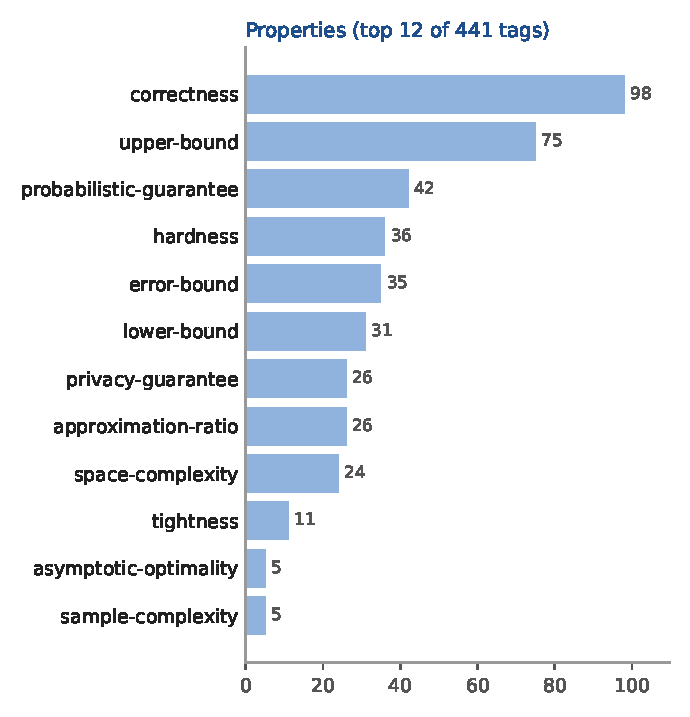
\includegraphics[width=.48\linewidth]{figures/f_props.pdf}\hfill
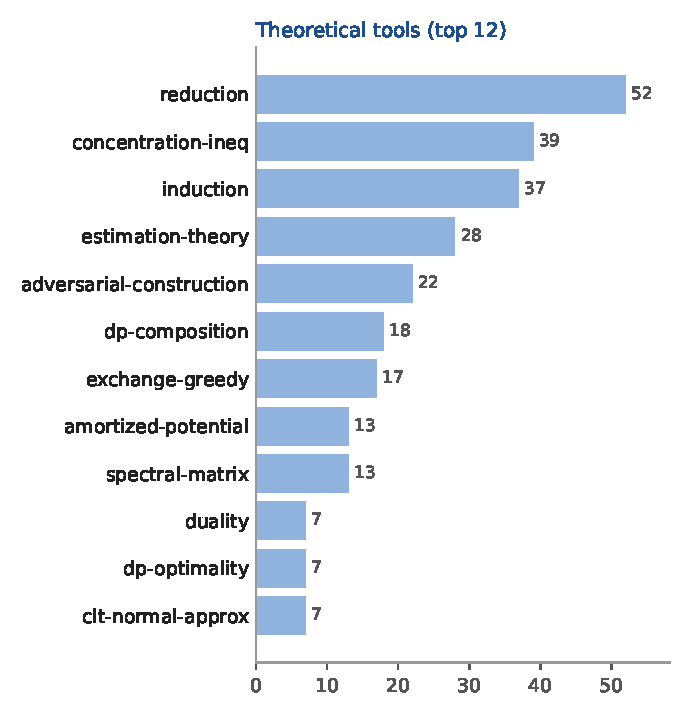
\includegraphics[width=.48\linewidth]{figures/f_tools.pdf}
\caption{Left: most-studied properties (top 12 of 441 property tags on the 228 tagged
papers). Right: most-used theoretical tools (top 12) --- each later chapter is one
tool.}\label{fig:props-tools}
\end{widefigure}

\section{Domains and dialects}
Figure~\ref{fig:domains-pairs} (left) shows where theory lives. Graph systems (56 papers)
are now the dominant dialect --- hardness $\to$ branch-and-bound and parameterized
algorithms $\to$ index-correctness lemmas. Privacy (26) is a near-monoculture of
composition accounting (69\% of its papers), increasingly in R\'enyi/f-DP currency.
Streaming and sketching splits into a pure-theory wing (matching lower bounds) and estimator
systems; vector search (25) splits between CLT-style certification and structural
correctness of graphs and routers.

\section{The playbook: property $\times$ tool pairings}
Figure~\ref{fig:domains-pairs} (right) is the survey's central cross-tab: which tool
delivers which property. The two workhorses are \textbf{hardness $\times$ reduction}
(32 papers) and \textbf{correctness $\times$ induction} (29). The pattern to
internalize: DB theory compresses into about eight such pairings, and each chapter of
these notes ends with the pairing(s) its tool owns.

\begin{widefigure}[htbp]
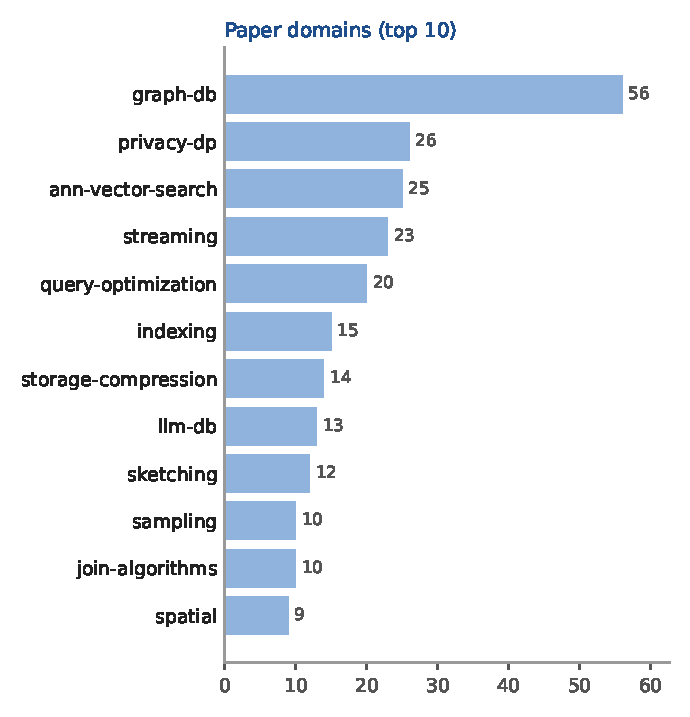
\includegraphics[width=.48\linewidth]{figures/f_domains.pdf}\hfill
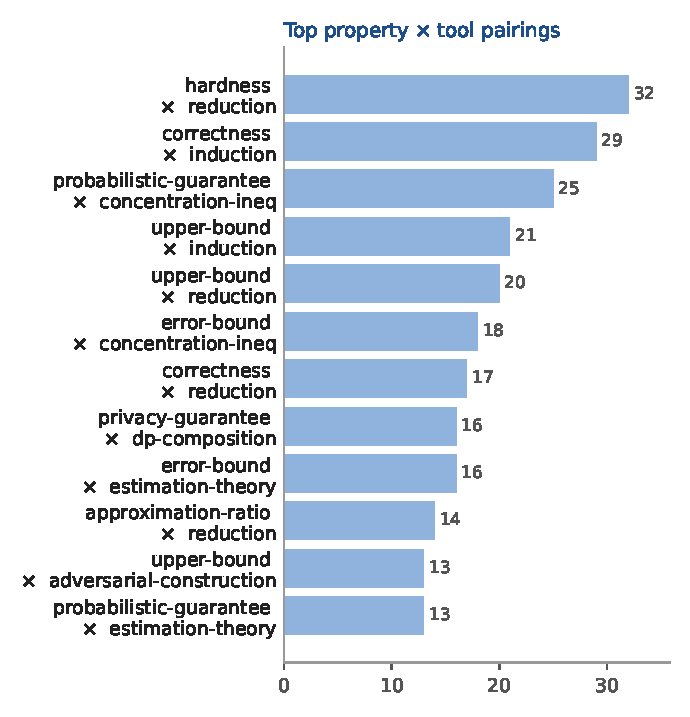
\includegraphics[width=.48\linewidth]{figures/f_pairs.pdf}
\caption{Left: paper domains (top 10). Right: top property$\times$tool pairings
(top 10) --- the ``playbook''.}\label{fig:domains-pairs}
\end{widefigure}

\section{Where theory sits}
66\% of tagged papers use theory as a \emph{design driver}; in 25\% the formal result
\emph{is} the paper (concentrated in the PODS issue and the pure streaming enclave);
motivation-only and evaluation-yardstick roles cover the rest. The role split matters
when reading exemplars: a design-driver paper proves what it builds; a
theory-as-contribution paper builds nothing and proves everything.

\section{Chapter map}
\label{ch:map}
Each of the following chapters is one tool: the formal core, then real SIGMOD~2026
exemplars with minimal context, then a ``when to reach for it'' box. Exemplars are
transcribed from the papers' own statements, with PODS-issue exemplars capped at one per
chapter (two for communication complexity, whose corpus presence is small); a paper may
recur in a second chapter when it is a clean exhibit of two tools --- each chapter
treats it under its own lens, and the \pods\ marker identifies PODS-issue exemplars in
the text.

\begin{widetable}[htbp]
\caption{Chapter map, ordered by how often the corpus uses each tool.
``Papers'' = tagged corpus papers using the tool; ``Ex.'' = exemplars
featured in the chapter.}
\label{tab:map}
\begin{tabular}{rllc}
\toprule
Ch. & Tool & Papers & Ex. \\
\midrule
1 & Reductions & 52 & 6 \\
2 & Concentration inequalities & 39 & 5 \\
3 & Induction & 37 & 6 \\
4 & Estimation theory & 28 & 6 \\
5 & Adversarial constructions & 22 & 6 \\
6 & DP composition & 18 & 6 \\
7 & Exchange--greedy arguments & 17 & 6 \\
8 & Spectral / matrix tools & 13 & 6 \\
9 & Amortized--potential analysis & 13 & 6 \\
10 & Coresets \& randomized NLA & 8 & 6 \\
11 & Information-theoretic bounds & 5 & 5 \\
12 & Communication complexity & 4 & 4 \\
13 & Online decisions (competitive \& regret) & 4 & 4 \\
\bottomrule
\end{tabular}
\end{widetable}

Tools not large enough for their own chapter in this corpus but worth knowing by name:
adversarial-adjacent duality/LP arguments (7 papers), dynamic programming optimality (7),
CLT/normal approximations (7), dyadic peeling (6), sketch mergeability theory (6),
balls-bins-hashing (5) --- several appear as guest stars inside the thirteen chapters.

\section{How these notes were made}
\label{sec:provenance}
The survey was scripted end to end: the 385-paper list came from OpenAlex, sources were
fetched (arXiv \TeX{} when available, ACM camera-ready PDFs otherwise), statements,
proofs, and bound sentences were machine-extracted (2{,}405 statements, 1{,}130 proofs),
and the 228 theory-relevant papers were tagged against the controlled vocabulary above;
every figure and count in this chapter is a direct aggregate of those tags.

These lecture notes are typeset with the \texttt{tufte-book} class of the
Tufte-\LaTeX{} project (Apache~2.0), as bundled in Boaz Barak's \texttt{panbook}
(MIT); the layout conventions --- margin-column learning objectives, themed remark and
recap blocks, end-of-proof markers, per-chapter references --- follow Barak's
\emph{Introduction to Theoretical Computer Science} notes (text licensed
CC~BY-NC-ND~4.0; we borrow the conventions only, no content). License notices for the
distributed class files ship with the sources.

\chapter{Reductions: Importing Hardness into Database Problems}
\label{ch:reduction}

Most ``impossible'' statements in database research are not proved from scratch: they are
\emph{imported}. A reduction exhibits a computable translation from a problem already
believed hard --- CLIQUE, Set Cover, inner-product estimation, hyperclique detection ---
into the problem at hand, so that any algorithm, approximation, private mechanism, or
sampler for the target would also solve the source. Reductions are the most used
theoretical tool in our SIGMOD'26 corpus: 50 of 228 tagged papers rely on them, and 32 of
those pair a reduction with an explicit hardness claim. They matter in both directions:
they delimit what any system can do (lower bounds, dichotomies, inapproximability) and,
run backwards, they turn new problems into old ones with known algorithms.

\section{The tool: mappings that preserve what you care about}

\begin{definition}[Polynomial-time many-one reduction]
Let $L_1, L_2$ be decision problems. We write $L_1 \le_m^p L_2$ if there is a
polynomial-time computable function $f$ with $x \in L_1 \iff f(x) \in L_2$ for all $x$.
If some NP-hard $L_1$ reduces to $L_2$, then $L_2$ is NP-hard: a polynomial-time
algorithm for $L_2$, composed with $f$, would decide $L_1$.
\end{definition}

This is the classical core \cite{reduction-bg2,reduction-bg1,reduction-bg3}, and it
already reaches into databases.

\begin{example}[Conjunctive-query evaluation is NP-complete]
Given $(G,k)$, build in polynomial time the database $D_G$ holding the edge relation of
$G$, and let $Q_k$ be the conjunctive query
\[
Q_k \;=\; \exists v_1 \dots \exists v_k \,.\, \bigwedge_{1 \le i < j \le k} E(v_i, v_j).
\]
Then $G$ has a $k$-clique iff $Q_k(D_G) \ne \emptyset$. Since CLIQUE is NP-complete, CQ
evaluation is NP-hard (and it lies in NP) --- the starting point of query-evaluation
complexity \cite{reduction-bg6}.
\end{example}

Decision-hardness is often not enough: DB problems carry objectives (cost, error,
latency), so the reduction must preserve \emph{quality}, not just yes/no membership.

\begin{definition}[$L$-reduction, i.e., approximation-preserving reduction]
Optimization problem $A$ L-reduces to $B$ if there are polynomial-time maps $f$
(instances) and $g$ (solutions) and constants $\alpha, \beta > 0$ such that, for every
instance $x$ of $A$, writing $c_A, c_B$ for the objective values:
(i)~$\mathrm{OPT}_B(f(x)) \le \alpha \cdot \mathrm{OPT}_A(x)$; and
(ii)~every solution $y$ of $f(x)$ maps to a solution $g(y)$ of $x$ with
$|c_A(g(y)) - \mathrm{OPT}_A(x)| \le \beta \cdot |c_B(y) - \mathrm{OPT}_B(f(x))|$.
\end{definition}

\begin{proposition}
If $A$ L-reduces to $B$ with constants $\alpha,\beta$ and $B$ admits a polynomial-time
$r$-approximation, then $A$ admits an $\alpha\beta r$-approximation. Hence hardness of
\emph{approximating} $A$ --- e.g., Set Cover's $\log n$ threshold under the Unique Games
Conjecture --- transfers to $B$ \cite{reduction-bg4,reduction-bg1}.
\end{proposition}

\begin{remark}[Fine-grained and conditional reductions]
When polynomial versus exponential time is too coarse, the source problem $H$ carries a
quantitative hypothesis (SETH, combinatorial Boolean matrix multiplication, hyperclique
detection, listing lower bounds) \cite{reduction-bg5}. The reduction must then track
parameters: an algorithm for $P$ with cost $c_P$ on instances produced by $f$ yields an
algorithm for $H$ of cost (cost of $f$) $+$ (number of calls) $\cdot\, c_P$, and the
hypothesis transfers whenever this beats the assumed lower bound in every parameter
regime.
\end{remark}

The same skeleton covers quantitative guarantees: replace ``algorithm'' by ``mechanism
or estimator with error $\alpha$,'' and the reduction lifts accuracy instead of time.
Figure~\ref{fig:reduction-skeleton} schematizes the two halves.

\begin{figure}[t]
\centering
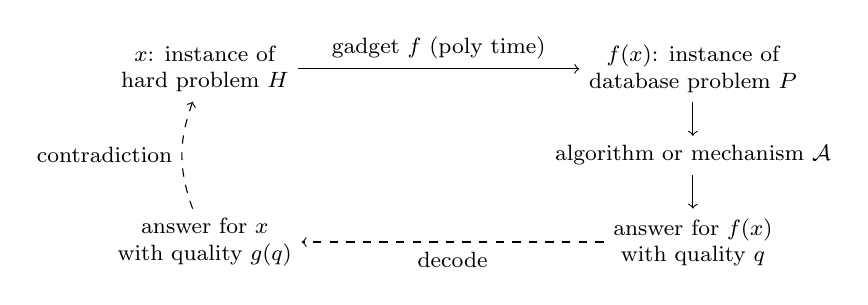
\begin{tikzpicture}[every node/.style={font=\footnotesize, align=center}]
  \node (xl) at (0,1.1) {$x$: instance of\\ hard problem $H$};
  \node (fl) at (6.2,1.1) {$f(x)$: instance of\\ database problem $P$};
  \node (al) at (6.2,0) {algorithm or mechanism $\mathcal{A}$};
  \node (dl) at (6.2,-1.1) {answer for $f(x)$\\ with quality $q$};
  \node (bl) at (0,-1.1) {answer for $x$\\ with quality $g(q)$};
  \draw[->] (xl) -- node[above] {gadget $f$ (poly time)} (fl);
  \draw[->] (fl) -- (al);
  \draw[->] (al) -- (dl);
  \draw[->,dashed] (dl) -- node[below] {decode} (bl);
  \draw[->,dashed] (bl) to[bend left=20] node[left] {contradiction} (xl);
\end{tikzpicture}
\caption{Every reduction has two halves: instances travel forward through the gadget;
solutions --- or accuracy, or privacy --- travel backward, so quality achieved for $P$
becomes quality for $H$.}
\label{fig:reduction-skeleton}
\end{figure}

\section{Reductions at work in the SIGMOD'26 corpus}

\subsection{Gadget reductions: privacy under continual release}

A stream of edge updates arrives over $T$ timesteps, and an $(\varepsilon,
\delta)$-differentially private mechanism must continually report, on $n$-node graphs,
the size of the maximum matching, the degree histogram, or the core number of a vertex.

\begin{theorem}[Continual-release lower bound]
Let $\varepsilon \in [0,1]$ and $\delta \in [0,1/3]$. Any $(\varepsilon, \delta)$-DP
incremental mechanism in the exact setting for maintaining the size of the maximum
matching, the degree histogram, or the core number of a vertex must have additive error
$\alpha = \Omega\bigl(\min\{ T^{a},\, n^{b} \}\bigr)$, for problem-specific constants
$a, b \in [1/8, 1/2]$.
\end{theorem}

The reduction embeds an \textsc{InnerProduct} instance of dimension $d$ into the update
stream via \emph{extendable bitwise-AND gadgets} with $v(d)$ vertices and $t(d)$ edges
(for matching, $v(d) = t(d) = O(d^2)$): a mechanism with additive error $\alpha$ would
answer the inner product within $2\alpha$, forcing
$\alpha = \Omega(\min\{ t^{-}(T), v^{-}(n) \})$ for generalized inverses, with $d$ chosen
exactly as that minimum. Binary-tree mechanisms with DP composition give near-matching
upper bounds, so the reduction is essentially tight. \cite{sigmod26-136}\pods

\subsection{Gap reductions: clustering with set outliers}

Points are clustered while whole \emph{sets} may be discarded as outliers: given points
$P$, a family $\mathcal{H}$ of candidate outlier sets (hyper-rectangles, or sets induced
by a relational join), and budgets $k, z$, choose at most $k$ centers and at most $z$
outlier sets so as to minimize the cost of the uncovered points.

\begin{theorem}[Inapproximability under the Unique Games Conjecture]
If the Unique Games Conjecture is true, there exists no $(1, f - \varepsilon,
\gamma)$-approximation algorithm that runs in polynomial time for the problem, whenever
$f = o(\log n)$, where the triple bounds the clustering-cost factor and the allowed
violation of the center and outlier budgets.
\end{theorem}

The reduction is a line--point encoding of Set Cover: element $x_i$ becomes the point
$p_i$ at coordinate $i$, each set $y$ becomes the outlier set $\{ p_i : x_i \in y \}$,
and singleton sets pad the family, so covering the element-points with at most $z$
outlier sets is exactly a set cover --- and Set Cover's UGC-conditional $\log n$
threshold crosses over. The same paper runs the machinery constructively: LP feasibility
with greedy rounding, weight-charging, and coresets yield $(2 + \varepsilon, 2,
O(1))$-approximations, including over acyclic joins. \cite{sigmod26-289}

\subsection{Coupon-collector reductions: sampling join--project queries}

For a join--project query $Q$ (a join followed by projection, so duplicates disappear),
with input size $N$ and output size $\mathsf{OUT}$, the paper asks what uniform sampling
from, and approximate counting of, $Q(I)$ must cost after indexing.

\begin{theorem}[Conditional bound for star queries]
For the star query $Q_k$, assuming the combinatorial hardness of listing star-join
results (any combinatorial listing algorithm requires
$\Omega(N \cdot \mathsf{OUT}^{1-1/k})$ time, under the property-testing model), no
combinatorial algorithm can preprocess an instance of input size $N$ and output size
$\mathsf{OUT}$ in $O(N \cdot \mathsf{OUT}^{1/k-\gamma})$ time and then return a uniform
sample from $Q(I)$ in $O(\mathsf{OUT}^{1/k+\gamma})$ expected time, for any constant
$\gamma > 0$.
\end{theorem}

The reduction runs the coupon collector backwards: a sampler this fast would list all
$\mathsf{OUT}$ results after $\mathsf{OUT} \log \mathsf{OUT}$ draws and thereby beat the
assumed listing lower bound. For the matrix query the hypothesis is instantiated by the
combinatorial hardness of Boolean matrix multiplication (the case $k=2$), and any
randomized algorithm that outputs an $O(1)$-approximation of $\mathsf{OUT}$ with high
probability requires at least $\Omega(N / \sqrt{\mathsf{OUT}})$ time; heavy/light
partitioning with Hoeffding intersection estimation gives matching upper bounds.
\cite{sigmod26-243}\pods

\subsection{Fine-grained reductions: direct access with min/max aggregates}

In direct access, the database is preprocessed once so that answers to an acyclic
free-connex conjunctive query can be enumerated in a user-chosen order with constant
delay; the question is which aggregate-driven orders, such as sorting by $\min X$, admit
quasilinear-time preprocessing.

\begin{theorem}[Hard side of the dichotomy]
Direct access according to $\min X$ is not possible in quasilinear time if $Q$ has a
chordless $k$-path ($k \ge 3$) between two variables in $X$, assuming the Hyperclique
hypothesis and SETH.
\end{theorem}

The reduction encodes triangle and hyperclique detection so that a quasilinear-time
direct-access structure for $\min X$ would decide hyperclique existence faster than the
hypothesis permits. The easy side of the dichotomy is algorithmic: strict total orders
are partitioned into partial orders that suitably rearranged join trees enforce, after
existential variables are eliminated in linear time. \cite{sigmod26-109}\pods

\begin{reachbox}{When to reach for reductions}
\begin{itemize}
\item \textbf{Lower bounds without a from-scratch proof.} Pick the canonical hard
problem closest in shape (Set Cover for covering and outlier budgets, InnerProduct for
private estimation, hyperclique detection for join patterns, listing for enumeration),
build a gadget, and state explicitly which hypothesis the reader inherits.
\item \textbf{Hardness of approximating, not just deciding.} Make the reduction
gap-preserving (an $L$-reduction), so the source's inapproximability threshold --- not
merely its NP-hardness --- crosses over to your objective.
\item \textbf{Fine-grained statements.} When the target is a refined running time
(sublinear, output-sensitive, constant delay), condition on a quantitative hypothesis
and audit the parameter blow-up of the gadget; a sloppy parameter map makes the bound
vacuous in some regime.
\item \textbf{Reductions also certify tractability.} The same machinery run backwards
--- encoding your problem into LP feasibility, matchings, or coresets --- builds the
upper-bound side of a dichotomy.
\end{itemize}
\end{reachbox}

\chapter{Concentration Inequalities}
\setcounter{section}{-1}   % sections start at 1.0 (see main.tex comment)
\label{ch:conc}

\begin{objectives}
\item Recognize when a component needs a \emph{whp} contract, and formalize the bad event.
\item Prove the ladder Markov $\to$ Chebyshev $\to$ Chernoff/Hoeffding, and match each rung
  to the dependence structure.
\item Tune per-event failure to $\delta/(\text{events})$; union-bound over all copies.
\item Dissect a paper's argument: random object, independence, rung, $\delta$ budget.
\end{objectives}

Concentration inequalities bound the probability that a random quantity strays far from
its expectation. For a systems paper they upgrade a randomized component that is correct
\emph{in expectation} --- a sampler, sketch, random walk, or noise mechanism --- into one
correct \emph{with high probability (whp)}: a quantified contract such as
``$(1\pm\varepsilon)$-accurate with probability $1-1/\operatorname{poly}(n)$'' or
``running time $O(T)$ with probability $1-1/N$.'' The recipe is constant: name the bad
event, bound it by a tail inequality, union-bound over all copies of the component. In the
SIGMOD'26 corpus this is among the most-used theoretical tools (38 tagged papers),
directly supplying the probabilistic-guarantee property in 25 of them.

This chapter presents the basic ladder and the standard exemplars first;
Section~\ref{sec:conc-advanced} adds the advanced rungs (martingales, two harder
exemplars) as extension reading.

\section{The tool: concentration inequalities}

The problem class is uniform across applications: we can compute (or bound) the
expectation of some random quantity $X$ --- the number of sampled points falling in a
region, the error of a private estimate, the load of a hash bucket --- but an algorithm
must succeed on the \emph{actual} draw, not the average. What concentration delivers is a
bound of the form
\[
\Pr\bigl[\,|X - \mathbb{E}X| \ge t\,\bigr] \;\le\; \text{some decreasing function of } t,
\]
plus the craft of making that function decrease fast enough. How fast is ``fast enough''
is the organizing question of this chapter: a bound of $\delta$ per bad event survives a
union bound over $1/\delta$ events, so a component replicated $\operatorname{poly}(n)$
times needs per-event failure $1/\operatorname{poly}(n)$, which in turn needs tails that
decay \emph{exponentially} in the deviation.

\begin{remarkbox}[Notation]
``whp'' (with high probability) always means probability at least
$1 - 1/\operatorname{poly}(n)$, or $1 - 1/N$ for a system of $N$ components; the
polynomial in the failure probability is set by the union bound over the whole system.
\end{remarkbox}

\subsection{The basic ladder}
\label{sec:conc-ladder}

Every bound in the family is Markov's inequality in disguise
\cite{concentration-ineq-bg5,concentration-ineq-bg6,concentration-ineq-bg7}.

\begin{theorem}[Markov]\label{thm:conc-markov}
Let $X \ge 0$ be a random variable with $\mathbb{E}X < \infty$. Then for every $a > 0$,
\[
\Pr[X \ge a] \;\le\; \frac{\mathbb{E}X}{a}. \eopm
\]
\end{theorem}

\begin{proof}
$\mathbb{E}X \ge \mathbb{E}[X \cdot \mathbf{1}\{X \ge a\}] \ge a\,\Pr[X \ge a]$; divide by $a$.
\end{proof}

One moment, one side, polynomial tail. Applying it to $(X-\mu)^2$ instead of $X$ gives the
two-sided, second-moment rung:

\begin{corollary}[Chebyshev]\label{cor:conc-chebyshev}
Let $\mu = \mathbb{E}X$ and $\operatorname{Var}(X) < \infty$. Then for every $t > 0$,
\[
\Pr[\,|X - \mu| \ge t\,] \;\le\; \frac{\operatorname{Var}(X)}{t^2}. \eopm
\]
\end{corollary}

\begin{proof}
Markov (Theorem~\ref{thm:conc-markov}) applied to the nonnegative variable $(X-\mu)^2$
with $a = t^2$.
\end{proof}

Polynomial tails suffice for constant success probability --- boosted to high probability
by repetition and medians --- but they cannot survive a union bound over
$\operatorname{poly}(n)$ events. Exponential tails come from applying Markov to
$e^{\lambda X}$:

\begin{lemma}[Chernoff method]\label{lem:conc-chernoff-method}
For any random variable $X$, any $a \in \mathbb{R}$ and any $\lambda > 0$,
\[
\Pr[X \ge a] \;=\; \Pr\bigl[e^{\lambda X} \ge e^{\lambda a}\bigr] \;\le\;
e^{-\lambda a}\,\mathbb{E}\bigl[e^{\lambda X}\bigr],
\]
and one optimizes over $\lambda > 0$ (the \emph{moment generating function} controls the
tail). \eop
\end{lemma}

\begin{proof}
Markov (Theorem~\ref{thm:conc-markov}) applied to the nonnegative variable
$e^{\lambda X}$ at level $a' = e^{\lambda a}$; the inequality is monotone in $\lambda$'s
sign, so only $\lambda > 0$ is useful.
\end{proof}

Evaluating the moment generating function of a sum of independent bounded variables
yields the two workhorses of randomized systems. The multiplicative form is the one to
memorize for sampling and sketching
\cite{concentration-ineq-bg1,concentration-ineq-bg5,concentration-ineq-bg7}:

\begin{theorem}[Chernoff, multiplicative form]\label{thm:conc-chernoff-mult}
Let $X_1,\dots,X_m$ be independent random variables with $X_i \in [0,1]$,
$X = \sum_{i=1}^m X_i$, $\mu = \mathbb{E}X$. Then for every $\varepsilon \in (0,1)$,
\[
\Pr[X \ge (1+\varepsilon)\mu] \;\le\; e^{-\varepsilon^2\mu/3},
\qquad
\Pr[X \le (1-\varepsilon)\mu] \;\le\; e^{-\varepsilon^2\mu/2}. \eopm
\]
\end{theorem}

\begin{proof}[Proof idea]
Chernoff method (Lemma~\ref{lem:conc-chernoff-method}) on $X$, then the elementary bound
$(1+\varepsilon)\ln(1+\varepsilon)-\varepsilon \ge \varepsilon^2/3$ (and its lower-tail
twin) on the optimized exponent; the full derivation is in the
Appendix (Section~\ref{sec:conc-appendix}).
\end{proof}

The additive form is interchangeable whenever the summands are bounded but not
naturally counts \cite{concentration-ineq-bg2,concentration-ineq-bg7,concentration-ineq-bg8}:

\begin{theorem}[Hoeffding, additive form]\label{thm:conc-hoeffding}
Let $X_1,\dots,X_m$ be independent with $X_i \in [a_i,b_i]$ a.s.\ and
$X = \sum_i X_i$. Then for every $t > 0$,
\begin{align*}
\Pr[X - \mathbb{E}X \ge t] \;&\le\;
\exp\!\Bigl(-\, \frac{2t^2}{\sum_i (b_i-a_i)^2}\Bigr),\\
\Pr[X - \mathbb{E}X \le -t] \;&\le\;
\exp\!\Bigl(-\, \frac{2t^2}{\sum_i (b_i-a_i)^2}\Bigr). \eopm
\end{align*}
\end{theorem}

\begin{proof}[Proof idea]
Chernoff method plus \emph{Hoeffding's lemma},
$\mathbb{E}[e^{\lambda(X_i - \mathbb{E}X_i)}] \le e^{\lambda^2(b_i-a_i)^2/8}$; optimize
$\lambda$ (proof in Section~\ref{sec:conc-appendix}).
\end{proof}

\begin{widefigure}[t]
\pgfplotsset{compat=1.15}
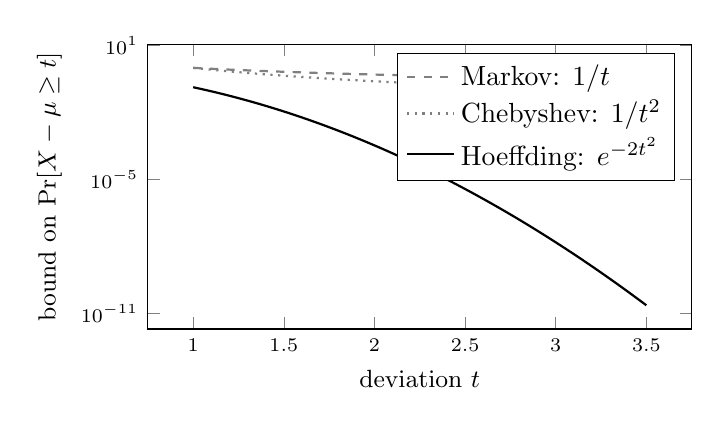
\begin{tikzpicture}
\begin{axis}[
  width=0.7\textwidth, height=5.2cm,
  xlabel={deviation $t$}, ylabel={bound on $\Pr[X-\mu \ge t]$},
  ymode=log, domain=1:3.5, samples=80,
  legend pos=north east, legend cell align=left,
  tick label style={font=\scriptsize}, label style={font=\small}
]
\addplot[gray, thick, dashed]  {1/x};
\addlegendentry{Markov: $1/t$}
\addplot[gray, thick, dotted]  {1/x^2};
\addlegendentry{Chebyshev: $1/t^2$}
\addplot[black, thick]         {exp(-2*x^2)};
\addlegendentry{Hoeffding: $e^{-2t^2}$}
\end{axis}
\end{tikzpicture}
\caption{Tail decay for a unit-scale random quantity: moment bounds fall polynomially,
independence buys the exponential curve --- the gap that makes
$\operatorname{poly}(n)$-way union bounds affordable.}
\label{fig:conc-tails}
\end{widefigure}

\sidenote{The entry fee for both forms is \emph{independence plus bounded summands}. The
tunable currency is the exponent --- $\varepsilon^2\mu$ or $2t^2/\sum_i(b_i-a_i)^2$ ---
which must be pushed past $\log(\text{\#events}/\delta)$ for the failure probability to
amortize. When the summands are unbounded but light-tailed (Gaussian, Laplace,
sub-exponential, sub-gamma), the same Chernoff-method machinery applies with a
moment-generating function that exists near $0$; corpus papers use sub-gamma tails for
approximate counters (Morris-type) and Laplace tails for privacy noise, and we will see
the latter in Section~\ref{sec:conc-ldp}.}

When independence fails but each random choice shifts the running statistic by a bounded
amount, the ladder has two more rungs --- Azuma--Hoeffding and McDiarmid --- built on
martingales; they are stated, with usage guidance, in
Section~\ref{sec:conc-advanced}.

\subsection{How to choose a rung}
\label{sec:conc-choose}

The selection procedure is mechanical once two questions are answered. \emph{First, what
depends on what?} If the random object is a sum of independent bounded indicators ---
samples retained, points in a region, hashed keys --- use multiplicative Chernoff when
the bound should be relative to the expectation $\mu$ (sampling rates, subsampling), and
additive Hoeffding when it should be relative to the range parameters
$b_i - a_i$ (weighted sums, real-valued measurements). \emph{Second, what moments are
available?} If only the mean (or an exponent-optimized mean of a transform) is
computable, Markov is the floor --- and, applied to $e^{\lambda X}$, it is secretly the
ceiling too.

\begin{reachbox}{When to Reach for Concentration}
Reach whenever a randomized component must be certified --- sampling/sketching estimators,
random walks, sampled data structures, hashing, privacy noise --- and the deliverable is a
probability-qualified contract: accuracy $(1\pm\varepsilon)$ whp, or time/space bounds
holding with probability $1-1/N$. Then run the recipe:
\begin{enumerate}
\item Name the random object $X$ and the bad event $\{|X - \mathbb{E}X| \ge t\}$.
\item Check the dependence structure: independent bounded summands $\to$
  Chernoff/Hoeffding; adaptive exposure or capped per-variable influence $\to$ the
  martingale rungs of Section~\ref{sec:conc-advanced}; only moments available $\to$
  Markov/Chebyshev --- constant probability, boostable by repetition with medians (and
  Markov on $e^{\lambda X}$ is the engine of every exponential-tail argument anyway).
\item Tune parameters so each bad event fails with probability at most
  $\delta/(\text{events})$ --- i.e.\ push the exponent past
  $\log(\text{events}/\delta)$; only exponential tails amortize over
  $\operatorname{poly}(n)$ copies, polynomial ones do not.
\item Union-bound over all copies of the component.
\end{enumerate}
\end{reachbox}

\section{Trimmed statistics in a turnstile stream}
\label{sec:conc-trimmed}

The exemplar is a PODS'26 paper on robust streaming statistics \cite{sigmod26-175}\pods.
Frequency moments, $F_p = \sum_i |x_i|^p$, are the workhorses of database analytics:
query optimization, data mining, and network monitoring all rely on them, and the
classical streaming results estimate them over the \emph{whole} frequency vector. Many
analytics tasks, however, want order-restricted quantities instead: statistics built from
only the heaviest (or the central) part of the data, with the extremes treated as
outliers --- the streaming analogue of the trimmed mean from robust statistics. The paper
studies such \emph{trimmed statistics} --- notably the $F_p$ moment of the top-$k$
coordinates, a Ky-Fan-type norm behind impact measures like the $h$-index --- in the
turnstile streaming model, and shows that for every $p \in [0,2]$ they can be estimated
in a single pass using $\operatorname{poly}(\log n/\varepsilon)$ bits of space.

\paragraph{Problem.}
Work in the \emph{strict turnstile} streaming model: an $n$-dimensional frequency vector
$\mathbf{x} \in \mathbb{Z}^n$ starts at zero and receives a long stream of updates of the
form ``add $\Delta$ to coordinate $i$'' (with $\Delta$ of either sign); the algorithm
sees updates one at a time and must answer queries about the final $\mathbf{x}$ using
space far less than $n$. Let $a_1,\dots,a_k$ be the $k$ coordinates of $\mathbf{x}$ of
largest absolute value. The \emph{trimmed statistic} of order $(p,k)$ is
$\sum_{i=1}^k |a_i|^p$ for $0 \le p \le 2$: the $F_p$ mass contributed by the top $k$
coordinates --- the part of the data that survives trimming away the tail. Such
statistics are the streaming analogue of trimmed estimators in robust statistics.

\paragraph{Guarantee.}

\begin{theorem}[Top-$k$ $F_p$ estimation, Theorem~4 of the paper]\label{thm:conc-trimmed}
Let $\mathbf{x} \in \mathbb{Z}^n$, $p \in [0,2]$, $k \ge 0$, $\varepsilon \in (0,1)$.
Suppose $\|\mathbf{x}_{-k}\|_2^2 \ge (\varepsilon/\log n)^c \cdot k$ for a constant $c$,
where $\mathbf{x}_{-k}$ excludes the top-$k$ coordinates. Then there exists a
\emph{linear sketch} using $\operatorname{poly}(\log n/\varepsilon)$ bits of space that
estimates $\sum_{i=1}^k |a_i|^p$ to a $(1\pm\varepsilon)$ factor with high constant
probability. \eop
\end{theorem}

\sidenote{A \emph{linear sketch} stores $A\mathbf{x}$ for a random matrix $A$; it is the
standard route to mergeable, one-pass, deletion-tolerant stream summaries. The condition
on $\|\mathbf{x}_{-k}\|_2^2$ holds automatically once $k \ge \operatorname{polylog} n$,
so the theorem covers the practically interesting regime.}

\paragraph{How concentration is applied.}
The algorithm partitions coordinates by magnitude into \emph{geometric level sets} whose
boundaries are shifted by a random offset $\zeta$ uniform in $[1/2,1]$, then
\emph{dyadically subsamples} each level: each coordinate of level $S_j$ is kept
independently with probability $r = \min\{1,\, C\log n/(\varepsilon^2 s_j)\}$ where
$s_j = |S_j|$ and $C$ is a constant. Survivors are found with a
CountSketch\footnote{CountSketch (Charikar--Chen--Farach-Colton) recovers, from hashed
counters, all coordinates whose value exceeds a $\theta$-fraction of the residual
$\ell_2$ norm (a \emph{heavy hitter} structure); the paper needs only this black box.}
fed with $\Theta(\log n)$ buckets per subsampling rate. The concentration step is the
following lemma; its random objects are the independent retention indicators $X_i$ of
the coordinates of $S_j$, each Bernoulli($r$), so the survivor count has mean $s_j r$.

\begin{lemma}[Level-size estimation, Lemma~4.4 of the paper, notation cleaned]
\label{lem:conc-trimmed-level}
Let $S_j$ be a level set with $s_j = |S_j|$, and subsample each coordinate independently
with probability $r = \min\{1,\, C\log n/(\varepsilon^2 s_j)\}$. If $z$ coordinates of
$S_j$ survive and $\tilde{s}_j = z/r$, then with probability $1 - 1/\operatorname{poly}(n)$,
\[
(1-\varepsilon)\,s_j \;\le\; \tilde{s}_j \;\le\; (1+\varepsilon)\,s_j . \eopm
\]
\end{lemma}

\begin{proof}[Proof sketch]
Write $u_1,\dots,u_{s_j}$ for the coordinates of $S_j$, and let $X_i$ be the indicator
that $u_i$ is sampled, so $\mathbb{E}\sum_i X_i = s_j r$. Multiplicative Chernoff gives
$\Pr[\,|\sum_i X_i - s_jr| \ge \varepsilon s_j r\,] \le
2\exp(-\varepsilon^2 s_j r/3) \le 2\exp(-C\log n/3) \le 1/\operatorname{poly}(n)$;
divide by $r$. (Full proof in Section~\ref{sec:conc-appendix}.)
\end{proof}

The $\delta$ tuning is explicit: $r$ is chosen exactly so that the Chernoff exponent
$\varepsilon^2 s_j r$ equals $C \log n$, i.e.\ per-level failure $1/\operatorname{poly}(n)$;
there are only $O(\log_{1+\varepsilon} m)$ levels (magnitude scales), so a union bound
over levels preserves the polynomial failure probability. A companion lemma (Lemma~4.5 of
the paper) uses the same Chernoff bound on the binomial survivor count to show that fewer
than $O(\log n/\varepsilon^2)$ coordinates survive per level whp --- which is what makes
the heavy-hitter structure, and hence the space bound,
$\operatorname{poly}(\log n/\varepsilon)$.

\paragraph{What it buys.}
The system gets a one-pass, sublinear-space summary of trimmed statistics --- robust
aggregate mass that ignores the tail --- with a certificate strong enough to union-bound
into larger algorithms; the randomness of the offset $\zeta$ (rather than an adversarial
grid) is what makes the level-set decomposition itself immune to worst-case input
placement.

\section{Maximum range sum by randomized grid shifting}
\label{sec:conc-maxrs}

The exemplar is a SIGMOD'26 paper on spatial query processing \cite{sigmod26-259}. The
\emph{maximum range sum} (MaxRS) problem sits behind every ``find the best location''
query: given weighted points --- customers, incidents, sensors --- and a fixed-size
geometric region $Q$, place $Q$ anywhere in space so that it captures as much total
weight as possible; that placement is where to site a store, a base station, or an
emergency facility. The problem is well studied by both the database and the
computational-geometry communities, and the paper revisits it in three practically
motivated variations: \emph{dynamic} MaxRS, where points are inserted and deleted and a
good placement must be maintained under updates; \emph{batched} MaxRS, where many query
regions must be answered at once; and \emph{colored} variants that group the points into
classes. Its headline results are a randomized $(\tfrac12-\varepsilon)$-approximation
for dynamic MaxRS with polylogarithmic update time --- the first algorithm of this kind
--- together with conditional lower bounds showing that the batched problem cannot be
solved substantially faster than the trivial approach.

\paragraph{Problem.}
In the \emph{maximum range sum} (MaxRS) problem, the input is a set $P$ of $n$ points in
$\mathbb{R}^d$, each carrying a weight, and a query shape $Q$ --- here a $d$-ball of
given radius. The goal is to place $Q$ (translate it anywhere) so as to maximize the
total weight of the points of $P$ covered.

Exact MaxRS is expensive: for $Q$ a $2$-ball the colored version carries a conditional
$\Omega(n^2)$ lower bound, and assuming that $(\min,+)$-convolution on length-$n$
sequences requires $\Omega(n^2)$ time, the batched variant on $n$ points and $m$ query
radii requires $\Omega(mn)$ time --- almost matching the trivial $O(mn\log n)$ upper
bound.

\sidenote{\emph{Conditional lower bound}: a reduction from $(\min,+)$-convolution ---
widely conjectured to need quadratic time --- transfers that hardness to MaxRS. This is
the paper's evidence that \emph{approximation} is necessary, and approximation is exactly
where concentration enters.}

\paragraph{Guarantee.}

\begin{theorem}[Static MaxRS, one representative case of the paper]\label{thm:conc-maxrs}
For static MaxRS with $Q$ a $d$-ball and any $0 < \varepsilon < 1/2$, there is a
randomized $(\tfrac12-\varepsilon)$-approximation algorithm running in time
$O(\varepsilon^{-2d-2} n \log n)$; the approximation factor holds with high probability,
i.e.\ $1 - n^{-\Omega(1)}$. The dynamic version achieves the same factor with amortized
update time $O(\varepsilon^{-2d-2}\log n)$. \eop
\end{theorem}

\paragraph{How concentration is applied.}
The algorithm randomly shifts a grid over the point set and, per cell, takes a random
sample of the cell's points; the candidate balls it examines are drawn from a finite set
of $k \le n$ possibilities determined by the shift. Two facts combine. First, a
\emph{geometric covering lemma}: if $C$ is a $d$-ball of radius $\rho$ and $B$ a unit
$d$-ball whose center lies at distance $\rho^2$ from the center of $C$, then the
$(d-1)$-dimensional measure of the cap $B \cap \partial C$ is at least a
$(\tfrac12 - \Theta(\varepsilon))$ fraction of the measure of $\partial C$ --- i.e., a
random point of $C$'s boundary lands in any fixed candidate ball with probability at
least $\tfrac12 - \Theta(\varepsilon)$. Second, the concentration step:

\begin{lemma}[Sampling concentration, Lemma of the paper, notation cleaned]
\label{lem:conc-maxrs-sample}
Let $S = \{p_1,\dots,p_t\}$ be such that each point of $S$ lies inside the candidate ball
$B$ independently with probability at least $\tfrac12 - \Theta(\varepsilon)$, and let
$Y_B = \sum_{i=1}^t \mathbf{1}\{p_i \in B\}$. Then with high probability,
simultaneously for all $k \le n$ candidate balls,
\[
Y_B \;\ge\; (1-\varepsilon)\Bigl(\tfrac12 - \Theta(\varepsilon)\Bigr)\,t . \eopm
\]
\end{lemma}

\begin{proof}[Proof sketch]
The $X_i = \mathbf{1}\{p_i \in B\}$ are independent indicators with
$\mathbb{E}[Y_B] \ge (\tfrac12 - \Theta(\varepsilon))t$; multiplicative Chernoff gives
$\Pr[Y_B < (1-\varepsilon)\mathbb{E}Y_B] \le e^{-\varepsilon^2 t/2}$, and a union bound
over the $k \le n$ balls keeps this whp provided
$t = \Theta(\varepsilon^{-2}\log n)$. (Full proof in
Section~\ref{sec:conc-appendix}.)
\end{proof}

The random objects are the per-point sampling/shift indicators; the structure is full
independence across points (the random shift acts independently per cell); the rung is
multiplicative Chernoff; and the $\delta$ tuning sets $t = \Theta(\varepsilon^{-2}
\log n)$ so each of the $n$ candidate balls fails with probability $n^{-\Omega(1)}$ ---
the same ``push the exponent past $\log(\text{events})$'' accounting as in
Section~\ref{sec:conc-trimmed}, with the exponent coming from sample size rather than
subsample rate.

\paragraph{What it buys.}
The spatial engine answers best-placement queries in near-linear time with a certified
$(1/2-\varepsilon)$ fraction of the optimum whp --- and supports updates in polylog
amortized time --- where exact computation faces (conditional) quadratic barriers. The
same Chernoff-plus-union-bound skeleton, re-instantiated with trapezoidal maps, gives the
paper's $(1-\varepsilon)$-approximation for the colored variant.

\section{User-level private query processing with sampled tuples}
\label{sec:conc-s4s}

The exemplar is a SIGMOD'26 paper on private query processing \cite{sigmod26-079}.
Answering select--join--aggregate (SJA) queries under differential privacy is a basic
building block of privacy-preserving analytics: the system must return an accurate
aggregate while guaranteeing that no adversary can confidently infer whether any one
\emph{user's} data was present or absent. The state of the art achieves strong,
instance-optimal accuracy at this \emph{user level}, but pays for it by solving
expensive optimization programs over the whole database --- prohibitive at scale.
Sampling is the classic escape hatch, buying a tunable trade-off between accuracy and
computational cost, yet combining it with private processing is subtle: it is unclear
\emph{what} to sample for the best accuracy under a given compute budget, and the
existing mathematical tool chains were not designed with sampling in mind. The paper
builds a scalable user-level-DP SJA engine that privately truncates each heavy user's
contribution and Poisson-samples tuples to accelerate the truncation search, with an
error analysis that cleanly separates sampling error from privacy noise.

\paragraph{Problem.}
Consider a select--project--join--aggregate workload over a relational instance whose
rows belong to \emph{users}, each user contributing many tuples. The privacy contract is
differential privacy at the granularity of users:

\begin{definition}[$\varepsilon$-differential privacy, user level]\label{def:conc-dp}
A randomized mechanism $M$ satisfies $\varepsilon$-\emph{differential privacy} if for all
\emph{neighboring} inputs $D,D'$ and all measurable sets $S$,
\[
\Pr[M(D) \in S] \;\le\; e^{\varepsilon}\,\Pr[M(D') \in S].
\]
For \emph{user-level} DP, ``neighboring'' means \emph{all} tuples of one user added or
removed --- much stricter than tuple-level DP.
\end{definition}

Unbounded per-user contributions then blow up sensitivity, so the system
\cite{sigmod26-079} truncates each user's contribution to a threshold $\tau$ chosen
privately by a search (sparse vector technique), and accelerates the search by
Poisson-sampling tuples at rate $q$ before privatizing.

\sidenote{Poisson sampling also \emph{amplifies} privacy: a mechanism that is
$\varepsilon$-DP on the sample is $(\varepsilon')$-DP on the full data with
$\varepsilon' = \ln(1 + q(e^{\varepsilon}-1)) < \varepsilon$; the paper's
Sample-and-Explore comparison baselines use this. The proof is a binomial tail
computation --- again concentration.}

\paragraph{Guarantee.}

\begin{theorem}[Error of the sampled truncation, Algorithm~2 of the paper, compressed]
\label{thm:conc-s4s}
The mechanism satisfies $(\varepsilon,0)$-DP. Let $n$ be the number of records, $m$ the
number of users, and $q$ the sample rate. Write $\tau^*(T) = \max_u \sum_{t \in T}
\mathbf{1}[u \prec t]$ for the true maximum per-user contribution, and
$\varepsilon_i^* \ge \varepsilon/L$ for the noise-calibration budget over the $L$
search iterations. With probability $1-\beta$, the released answer $\hat{f}(T)$ obeys
\[
\bigl|\hat{f}(T) - f(T)\bigr| \;=\;
\widetilde{O}\Bigl(\sqrt{\textstyle\frac{n}{q}} + \frac1q +
\frac{1}{\varepsilon_i^*}\Bigl(\tau^*(T) + \sqrt{\textstyle\frac{\tau^*(T)}{q}}\Bigr)\Bigr),
\]
where $\widetilde{O}(\cdot)$ hides constants and polylogarithmic factors in $m$ and
$1/\beta$. \eop
\end{theorem}

\paragraph{How concentration is applied.}
The random objects are the independent sampling indicators
$\mathbf{1}\{t \text{ sampled}\} \sim \mathrm{Bernoulli}(q)$ over the $n$ tuples. The
sampled statistic $f(S) = \sum_{t \in T} w_t \mathbf{1}[t \text{ sampled}]$ satisfies
$\mathbb{E}[f(S)] = q\,f(T)$ and
$\operatorname{Var}[f(S)] = q(1-q)\sum_t w_t^2 \le qn$: a sum of independent bounded
variables with an explicit variance proxy --- the territory of the Bernstein/Chernoff
rung, whose bound gives $|f(S) - qf(T)| \lesssim \sqrt{qn \log(3L/\beta)}$ with
probability $1 - \beta/(3L)$; dividing by $q$ yields the $\sqrt{n/q}$ term. The
$\delta$-budgeting is again structural: the truncation-threshold search runs $L$
iterations, each is allocated failure probability $\beta/(3L)$, and a union bound over
iterations upgrades the per-iteration bound to the global $1-\beta$ contract --- with the
same per-event log factor $\log(3L/\beta)$ appearing inside the noise scale. The
$\tau^*(T)/\varepsilon_i^*$ terms come from the Laplace-style calibration of the final
release against the (privately learned) per-user cap.

\paragraph{What it buys.}
The query engine can offer user-level --- not merely tuple-level --- privacy at a
modest accuracy price: the sampling error $\sqrt{n/q}$ decouples from the privacy noise,
so tuning $q$ trades compute for accuracy without touching the privacy guarantee, and
the explicit $\tau^*(T)$ dependence quantifies exactly how much heavy user-contributors
cost the answer.

\section{Advanced usage and further reading}
\label{sec:conc-advanced}

Everything so far needs independence. Two extensions belong in every practitioner's
backpack: the martingale rungs that replace independence with bounded per-step
influence, and the light-tailed regime where summands are unbounded but have a moment
generating function. This section states the rungs, sketches two harder exemplars, and
points to the literature.

\subsection{Martingale rungs: Azuma--Hoeffding and McDiarmid}
\label{sec:conc-martingales}

Expose the randomness sequentially and book the shifts as a
\emph{martingale}\footnote{Recall: a martingale difference sequence $(Y_i)$ with respect
to a filtration $(\mathcal{F}_i)$ has $\mathbb{E}[Y_i \mid \mathcal{F}_{i-1}] = 0$; the
partial sums $M_j = \sum_{i\le j} Y_i$ then satisfy $\mathbb{E}[M_j \mid
\mathcal{F}_{j-1}] = M_{j-1}$.}:

\begin{theorem}[Azuma--Hoeffding]\label{thm:conc-azuma}
Let $(Y_i)_{i=1}^m$ be a martingale difference sequence with $|Y_i| \le c_i$ a.s. Then
for every $t > 0$,
\[
\Pr\Bigl[\textstyle\sum_{i=1}^m Y_i \ge t\Bigr] \;\le\;
\exp\!\Bigl(-\, \frac{t^2}{2\sum_{i=1}^m c_i^2}\Bigr). \eopm
\]
\end{theorem}

\begin{proof}[Proof idea]
Chernoff method on $\sum_i Y_i$, Hoeffding's lemma applied to each $Y_i$
\emph{conditionally on the past} (boundedness is all that is needed; independence is
replaced by iterated conditioning), then optimize $\lambda$
(Section~\ref{sec:conc-appendix}).
\end{proof}

The function-of-independent-variables form is the rung most used for adaptive
algorithms and data structures, where the analyzed quantity is not a sum but a function
whose per-variable influence is capped
\cite{concentration-ineq-bg4,concentration-ineq-bg5,concentration-ineq-bg6}:

\begin{theorem}[McDiarmid, bounded differences]\label{thm:conc-mcdiarmid}
Let $X_1,\dots,X_m$ be independent random variables and
$f\colon \prod_i \mathcal{X}_i \to \mathbb{R}$ a measurable function satisfying the
bounded differences condition: for each $i$ there is $c_i \ge 0$ with
\[
\bigl|f(x_1,\dots,x_i,\dots,x_m) - f(x_1,\dots,x_i',\dots,x_m)\bigr| \;\le\; c_i
\]
for all inputs and all $x_i'$. Then for every $t > 0$,
\[
\Pr\bigl[f(X_1,\dots,X_m) - \mathbb{E}f \ge t\bigr] \;\le\;
\exp\!\Bigl(-\, \frac{2t^2}{\sum_{i=1}^m c_i^2}\Bigr). \eopm
\]
\end{theorem}

\begin{proof}[Proof idea]
Apply Azuma--Hoeffding (Theorem~\ref{thm:conc-azuma}) to the \emph{Doob martingale}
$Y_i = \mathbb{E}[f \mid X_1,\dots,X_i] - \mathbb{E}[f \mid X_1,\dots,X_{i-1}]$, whose
increments are bounded by $c_i$ exactly because changing $X_i$ moves $f$ by at most
$c_i$ (Section~\ref{sec:conc-appendix}).
\end{proof}

\emph{When these rungs earn their keep.} If the algorithm is \emph{adaptive} --- later
random choices conditioned on earlier estimates, sampling without replacement, stopping
times --- the summands are dependent but each step's effect is bounded, and
Azuma--Hoeffding applies. If the quantity is a \emph{function} of many independent
inputs (a data structure's quality, a clustering cost, a query plan's runtime) with
per-input influence at most $c_i$, McDiarmid converts that directly. Hashing with
limited independence is the classic gap: the indicators are not fully independent, but
exposure by hash key gives bounded increments.

\subsection{Two advanced exemplars, sketched}
\label{sec:conc-ldp}

Both exemplars of this section are privacy papers that push past the
sum-of-independent-bounded-summands regime; each is sketched in one paragraph, and the
round-by-round argument of the first is transcribed in the
Appendix (Section~\ref{sec:conc-appendix}).

\paragraph{Private graph pattern counting under LDP \cite{sigmod26-012}.}
Counting subgraph patterns --- triangles, paths, stars --- is a cornerstone of network
analysis (community detection, fraud detection), and releasing such counts leaks
information about individual edges. Under \emph{local} differential privacy there is no
trusted curator: each node of the graph randomizes its own messages before anything is
aggregated, and existing LDP mechanisms were ad hoc, handling only specific patterns
such as triangles and stars. The paper gives the first general mechanism for counting
arbitrary \emph{acyclic} patterns under LDP. It runs $k$ rounds of message passing,
adding fresh Laplace noise --- \emph{sub-exponential} tails, so the Chernoff method
still applies --- at every node in every round. The $\delta$-accounting is the recipe of
Section~\ref{sec:conc-choose} in its purest form: failure budget $\beta'/N$ per node
per round, union bound over the $kN$ node-rounds, then an \emph{induction on rounds}
that grows the noise scale geometrically but controllably. The resulting estimate is
unbiased with error $\widetilde{O}(\sqrt{N\,d(G)^{k-1}})$ --- the square root of the
maximal possible count. For simple paths, the tail is only polynomial in $1/\beta$
(a variance/Markov argument), illustrating the price of dropping exponential tails.

\label{sec:conc-product}
\paragraph{Product noise as a concentration bound \cite{sigmod26-196}.}
Adding calibrated noise to a released statistic is the most fundamental route to
differential privacy: the system outputs $f(x) + \mathbf{n}$, and the guarantee rests
on the tail of the \emph{privacy-loss random variable} $L_M = \ln\frac{dP}{dQ}$ ---
$(\varepsilon,\delta)$-DP holds exactly when $\Pr[L_M \ge \varepsilon] \le \delta$,
a tail bound in disguise. For Gaussian noise $L_M$ is itself a univariate Gaussian,
and this is where standard analyses stop. The paper instead exploits the spherical
symmetry of typical noise distributions to generate $\mathbf{n}$ from a
\emph{product} of two independent components --- a radius controlling the noise
magnitude and a direction controlling its angle relative to the sensitivity vector
--- which re-expresses $L_M$ as a product measure and lets the tail be optimized
directly. The paper never writes the word ``Chernoff,'' but its argument --- factorize
$L_M$ into independent terms, bound $\mathbb{E}[U^q]$ for a transform $U$, and
\emph{minimize the resulting $\delta$ over the exponent $q$} --- is exactly the
Chernoff method (Lemma~\ref{lem:conc-chernoff-method}) on a likelihood ratio. The
payoff: expected noise smaller by a $\Theta(\log(1/\delta))$ factor than the Gaussian
mechanism at equal privacy.

\subsection{Further reading}

\begin{itemize}
\item Boucheron, Lugosi, and Massart \cite{concentration-ineq-bg5} --- the comprehensive
non-asymptotic treatment; the martingale and supremum versions live here.
\item Dubhashi and Panconesi \cite{concentration-ineq-bg6} --- the
randomized-algorithms viewpoint, with the exposure/Doob-martingale technique foregrounded.
\item Mitzenmacher and Upfal \cite{concentration-ineq-bg8} --- textbook treatment with
CS applications and all the Chernoff variants used in systems papers.
\item The originals: Chernoff (1952) \cite{concentration-ineq-bg1}, Hoeffding (1963)
\cite{concentration-ineq-bg2}, Azuma (1967) \cite{concentration-ineq-bg3}, and
McDiarmid's bounded-differences survey \cite{concentration-ineq-bg4}.
\item For a two-page refresher with proofs of the additive forms, the Stanford CS229
notes \cite{concentration-ineq-bg7}.
\end{itemize}

\begin{recap}
\item \textbf{What the tool is.} Concentration inequalities convert expectations into
  with-high-probability contracts: $\Pr[|X - \mathbb{E}X| \ge t]$ bounded by a tail
  function, tuned so that per-event failure $\delta/(\text{events})$ survives a union
  bound over all copies of the randomized component.
\item \textbf{Which rung when.} Independent bounded indicators/sums: multiplicative
  Chernoff (relative error) or additive Hoeffding (range-based). Adaptive or dependent
  exposure with bounded per-step effect: Azuma--Hoeffding. Function of many independent
  inputs with capped per-input influence: McDiarmid. Only moments available: Markov and
  Chebyshev --- constant-probability results, boostable by medians. Light-tailed
  unbounded noise (Laplace, Gaussian, sub-gamma): the Chernoff method still applies via
  the moment generating function.
\item \textbf{Why exponential tails.} Only $e^{-\Omega(\text{exponent})}$ tails make
  $\operatorname{poly}(n)$-way union bounds affordable; polynomial tails ($1/t$,
  $1/t^2$) cannot amortize --- visible in the corpus as the gap between
  $\widetilde{O}(\cdot)$ guarantees (Laplace/Chernoff paths) and $1/\beta$-type errors
  (variance-only paths).
\item \textbf{What the corpus showed.} Trimmed-statistic sketching
  (Section~\ref{sec:conc-trimmed}): Chernoff on subsampling survivors, union over
  $O(\log_{1+\varepsilon} m)$ levels. Spatial MaxRS (Section~\ref{sec:conc-maxrs}):
  Chernoff on sampled point-in-ball indicators, union over $\le n$ candidate balls.
  User-level private queries (Section~\ref{sec:conc-s4s}): Bernstein/Chernoff on
  Bernoulli-sampled sums with $\beta/(3L)$ budgets over search iterations.
\item \textbf{Advanced usage.} The martingale rungs
  (Section~\ref{sec:conc-martingales}) replace independence with bounded per-step
  influence; the privacy exemplars of Section~\ref{sec:conc-ldp} run the Chernoff
  method on Laplace noise and on a likelihood ratio. Long proofs of everything
  deferred live in the Appendix (Section~\ref{sec:conc-appendix}).
\end{recap}

\section{Appendix}
\label{sec:conc-appendix}

Proofs omitted from the main text are collected here.

\subsubsection*{Proof of Theorem~\ref{thm:conc-chernoff-mult} (Chernoff, multiplicative form)}
{\itshape Statement (recalled).} Let $X_1,\dots,X_m$ be independent with
$X_i \in [0,1]$, $X = \sum_i X_i$, $\mu = \mathbb{E}X$. Then
$\Pr[X \ge (1+\varepsilon)\mu] \le e^{-\varepsilon^2\mu/3}$ and
$\Pr[X \le (1-\varepsilon)\mu] \le e^{-\varepsilon^2\mu/2}$.\eop

\begin{proof}
By the Chernoff method (Lemma~\ref{lem:conc-chernoff-method}), for $\lambda > 0$,
$\Pr[X \ge (1+\varepsilon)\mu] \le e^{-\lambda(1+\varepsilon)\mu}
\prod_i \mathbb{E}[e^{\lambda X_i}]$. For $X_i \in [0,1]$ independence gives
$\mathbb{E}[e^{\lambda X_i}] = 1 + p_i(e^{\lambda}-1) \le
\exp(p_i(e^{\lambda}-1))$, so the product is at most $e^{\mu(e^\lambda - 1)}$ and,
choosing $\lambda = \ln(1+\varepsilon)$,
\[
\Pr[X \ge (1+\varepsilon)\mu] \;\le\;
\Bigl(\frac{e^{\varepsilon}}{(1+\varepsilon)^{1+\varepsilon}}\Bigr)^{\mu}
\;\le\; e^{-\varepsilon^2\mu/3},
\]
using $(1+\varepsilon)\ln(1+\varepsilon) - \varepsilon \ge \varepsilon^2/3$ for
$\varepsilon \in (0,1)$. The lower tail is symmetric, with exponent
$\varepsilon^2/2$.
\end{proof}

\subsubsection*{Proof of Theorem~\ref{thm:conc-hoeffding} (Hoeffding, additive form)}
{\itshape Statement (recalled).} Let $X_1,\dots,X_m$ be independent with
$X_i \in [a_i,b_i]$ a.s.\ and $X = \sum_i X_i$. Then for every $t > 0$,
$\Pr[X - \mathbb{E}X \ge t] \le \exp(-2t^2/\sum_i (b_i-a_i)^2)$, and the same for the
lower tail.\eop

\begin{proof}
\emph{Hoeffding's lemma}: if $Y \in [a,b]$ a.s.\ and $\mathbb{E}Y = 0$, then
$\mathbb{E}[e^{\lambda Y}] \le e^{\lambda^2(b-a)^2/8}$. (Proof: $e^{\lambda y}$ is
convex, so $e^{\lambda Y} \le \frac{b-Y}{b-a}e^{\lambda a} + \frac{Y-a}{b-a}e^{\lambda
b}$ pointwise; take expectations and minimize over a shifted $\lambda$.) Applying the
lemma to each centered summand and multiplying by independence,
$\mathbb{E}[e^{\lambda(X - \mathbb{E}X)}] \le e^{\lambda^2 \sum_i (b_i-a_i)^2/8}$; the
Chernoff method then gives
$\Pr[X - \mathbb{E}X \ge t] \le e^{-\lambda t + \lambda^2\sum(b_i-a_i)^2/8}$, and
optimizing at $\lambda = 4t/\sum(b_i-a_i)^2$ yields the stated
$e^{-2t^2/\sum(b_i-a_i)^2}$.
\end{proof}

\subsubsection*{Proof of Theorems~\ref{thm:conc-azuma} and~\ref{thm:conc-mcdiarmid} (martingale rungs)}
{\itshape Statement (recalled).} (i) If $(Y_i)_{i=1}^m$ is a martingale difference
sequence with $|Y_i| \le c_i$ a.s., then $\Pr[\sum_i Y_i \ge t] \le
\exp(-t^2/2\sum_i c_i^2)$. (ii) If $f$ has bounded differences $(c_i)$ over independent
$X_1,\dots,X_m$, then $\Pr[f - \mathbb{E}f \ge t] \le
\exp(-2t^2/\sum_i c_i^2)$.\eop

\begin{proof}
Let $M_j = \sum_{i \le j} Y_i$ with $\mathbb{E}[Y_i \mid \mathcal{F}_{i-1}] = 0$ and
$|Y_i| \le c_i$. Iterated conditioning gives
$\mathbb{E}[e^{\lambda M_m}] = \mathbb{E}[e^{\lambda M_{m-1}}
\mathbb{E}[e^{\lambda Y_m} \mid \mathcal{F}_{m-1}]]$, and \emph{conditionally on
$\mathcal{F}_{m-1}$} the variable $Y_m$ is centered and bounded in an interval of length
$2c_m$, so Hoeffding's lemma applies with $(b-a) = 2c_m$. Unrolling,
$\mathbb{E}[e^{\lambda M_m}] \le e^{\lambda^2\sum c_i^2/2}$, and optimizing $\lambda$
gives the stated tail. For McDiarmid, set $Y_i = \mathbb{E}[f \mid X_1,\dots,X_i] -
\mathbb{E}[f \mid X_1,\dots,X_{i-1}]$: this is a martingale difference sequence with
$|Y_i| \le c_i$ precisely because resampling only $X_i$ moves $f$ by at most $c_i$
(take conditional expectations over the two values of $X_i$), and
$\sum_i Y_i = f - \mathbb{E}f$. Azuma--Hoeffding applied to $(Y_i)$ is McDiarmid's
inequality.
\end{proof}

\subsubsection*{Proof of Lemma~\ref{lem:conc-trimmed-level} (level-size estimation,
Section~\ref{sec:conc-trimmed})}
{\itshape Statement (recalled).} Subsample each coordinate of a level set $S_j$,
$|S_j| = s_j$, independently with probability $r = \min\{1, C\log n/(\varepsilon^2
s_j)\}$. If $z$ coordinates survive, then $\tilde{s}_j = z/r$ satisfies
$(1-\varepsilon)s_j \le \tilde{s}_j \le (1+\varepsilon)s_j$ with probability
$1 - 1/\operatorname{poly}(n)$.\eop

\begin{proof}
Denote the coordinates of $S_j$ by $u_i$, $i \in [s_j]$, and let $X_i$ be the indicator
that $u_i$ is sampled into substream $P$, so the $X_i$ are independent with
$\mathbb{E}[X_i] = r$ and $\mathbb{E}\sum_i X_i = s_j r$. Multiplicative Chernoff
(Theorem~\ref{thm:conc-chernoff-mult}) gives
\begin{align*}
\Pr\Bigl[\Bigl|\textstyle\sum_i X_i - s_j r\Bigr| \ge \varepsilon s_j r\Bigr]
\;&\le\; 2\exp(-\varepsilon^2 s_j r/3)
\;\le\; 2\exp(-C\log n/3)\\
\;&\le\; 1/\operatorname{poly}(n),
\end{align*}
where the second inequality uses $s_j r = C\log n/\varepsilon^2$ (when the minimum in
the definition of $r$ is attained at this branch; otherwise $r = 1$ and there is nothing
to estimate). Dividing by $r$ converts the event into
$(1-\varepsilon)s_j \le \tilde{s}_j \le (1+\varepsilon)s_j$.
\end{proof}

\subsubsection*{Proof of Lemma~\ref{lem:conc-maxrs-sample} (sampling concentration,
Section~\ref{sec:conc-maxrs})}
{\itshape Statement (recalled).} If each point of $S = \{p_1,\dots,p_t\}$ lies in the
candidate ball $B$ independently with probability at least
$\tfrac12 - \Theta(\varepsilon)$, then simultaneously for all $k \le n$ candidate
balls, $Y_B = \sum_i \mathbf{1}\{p_i \in B\} \ge
(1-\varepsilon)(\tfrac12 - \Theta(\varepsilon))t$ whp.\eop

\begin{proof}
Fix a candidate ball $B$ and let $X_i = \mathbf{1}\{p_i \in B\}$; the $X_i$ are
independent, and by the covering property $\mathbb{E}[Y_B] = \sum_i \mathbb{E}X_i \ge
(\tfrac12 - \Theta(\varepsilon))t$. Multiplicative Chernoff gives
\[
\Pr\bigl[Y_B < (1-\varepsilon)\mathbb{E}Y_B\bigr] \;\le\;
e^{-\varepsilon^2 \mathbb{E}Y_B/2} \;\le\; e^{-\Theta(\varepsilon^2 t)}.
\]
With $t = \Theta(\varepsilon^{-2}\log n)$ this is $n^{-\Omega(1)}$ per ball, and a union
bound over the $k \le n$ candidate balls gives the simultaneous statement
$Y_B \ge (1-\varepsilon)(\tfrac12-\Theta(\varepsilon))t$ for all of them, with high
probability.
\end{proof}

\subsubsection*{Round-by-round noise control (Section~\ref{sec:conc-ldp})}
{\itshape Statement (recalled).} The $k$-round walk mechanism of \cite{sigmod26-012} is
unbiased for the walk count $W_k$ and, with probability $1-\beta$, errs by at most
$k\gamma\sqrt{N}\,(d(G)+\gamma)^{k-1}$, where
$\gamma = 2k\sqrt{8\log(2kN/\beta)}/\varepsilon$.\eop

\begin{proof}
Write $X_i^{(\ell)}$ for node $i$'s round-$\ell$ value. The mechanism gives, for each
node $i$ and round $\ell \in \{1,\dots,k\}$,
\[
X_i^{(\ell)} \;=\; \sum_{j \in N(i)} X_j^{(\ell-1)} \;+\;
\mathrm{Lap}\bigl(2k\|X^{(\ell-1)}\|_\infty/\varepsilon\bigr),
\]
so $\sum_{j\in N(i)} X_j^{(\ell-1)} \le d(G)\,\|X^{(\ell-1)}\|_\infty$ always. Allocate
failure $\beta'/N$ per node per round: the Laplace tail
$\Pr[\mathrm{Lap}(b) > u] \le \tfrac12 e^{-u/b}$ gives, with probability
$1-\beta'/N$ per node-round,
$2k\,\mathrm{Lap}(\|X^{(\ell-1)}\|_\infty/\varepsilon) \le
\gamma \|X^{(\ell-1)}\|_\infty$ for the stated $\gamma$ (with
$\beta' \approx \beta/k$). Union-bounding over the $\le kN$ node-rounds, all these
events hold simultaneously with probability $\ge 1-(k-1)\beta'$, and on that event an
induction gives
\[
\|X^{(\ell)}\|_\infty \;\le\; \bigl(d(G)+\gamma\bigr)\,\|X^{(\ell-1)}\|_\infty
\quad\Longrightarrow\quad
\|X^{(\ell)}\|_\infty \;\le\; \bigl(d(G)+\gamma\bigr)^{\ell}
\]
for all $\ell \le k-1$. The released count aggregates the $N$ per-node values, whose
centered Laplace contributions are independent sub-exponential variables each of scale
at most $O(\gamma(d(G)+\gamma)^{k-1})$; their sum concentrates around zero at scale
$\sqrt{N}\cdot\widetilde{O}(\gamma(d(G)+\gamma)^{k-1})$ by the same Chernoff-method
argument applied to light-tailed variables, which yields the stated
$k\gamma\sqrt{N}(d(G)+\gamma)^{k-1}$ error radius with probability $1-\beta$.
\end{proof}

\bibliographystyle{plainnat}
\bibliography{chapters/concentration-ineq-all}

\chapter{Induction and Invariants}

Induction is the workhorse that never gets top billing. In our tagged SIGMOD'26 corpus, 36 of 228 papers use it (the \#3 tool overall); the pairing \emph{correctness}~$\times$~\emph{induction}, with 29 papers, is the single most frequent property--tool co-occurrence in the survey, and induction also powers the \emph{upper-bound} pairing in 21 papers. The characteristic shape is not one grand named theorem but thousands of small, unnamed invariants --- half-page lemmas saying that one more elimination step, recursive call, or rewrite keeps a component consistent. Induction is thus the instrument of \emph{component} correctness: each cache, rewrite rule, or decomposition step is verified locally, and the global guarantee is assembled from the local ones.

\section{The Tool: Induction on What?}

Every inductive argument in the corpus answers two questions: what do we induct on, and what is preserved at each step?

\paragraph{Induction on what?} Three substrates dominate.

\begin{enumerate}
\item \textbf{Execution steps.} An algorithm induces a sequence of states $s_0, s_1, \dots, s_t$, one per operation (a function call, an elimination, a rewrite). One proves a state predicate $I$ --- the \emph{invariant} --- by induction on $i$: $I(s_0)$ holds, and each operation preserves $I$, so $I$ holds in every reachable state and implies the specification at final states. This is the inductive-assertion method of Floyd~\cite{induction-bg1} and Hoare~\cite{induction-bg2}, the loop-invariant discipline of algorithms texts~\cite{induction-bg4}, and Manna--Pnueli \emph{safety} reasoning: nothing bad ever becomes true~\cite{induction-bg3}.
\item \textbf{Structural recursion.} The object is built recursively --- a tree decomposition, an elimination forest, a recursive pseudo-tree, a hierarchy --- and the property is proved on the whole from the property on the parts. The database workhorse is \emph{leaf-peeling}: remove a leaf bag or leaf vertex, apply the induction hypothesis to the smaller object, then extend by one step.
\item \textbf{A natural-number measure.} Strong induction on a quantity that strictly decreases: the number of eliminated nodes, the number of bags, or the length of a rewrite sequence; structural induction is routinely converted into this form by choosing a measure~\cite{induction-bg5}.
\end{enumerate}

\begin{example}[Invariant preservation]
Given a set of states $\Sigma$, an initial state $s_0$, and a set of operations $\Gamma$, a predicate $I \subseteq \Sigma$ is an \emph{invariant} if (i) $I(s_0)$ holds, and (ii) whenever $I(s)$ holds and $s'$ results from applying an operation of $\Gamma$ to $s$, then $I(s')$ holds. By induction on the number of executed operations, every reachable state satisfies $I$; any property implied by $I$ at final states is therefore guaranteed.
\end{example}

\begin{center}
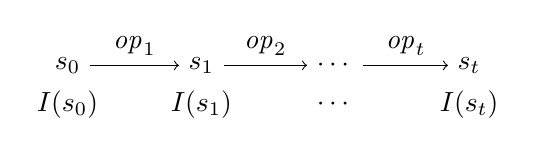
\begin{tikzpicture}
\node (s0) at (0,0)   {$s_0$};
\node (s1) at (1.7,0) {$s_1$};
\node (d)  at (3.4,0) {$\cdots$};
\node (st) at (5.1,0) {$s_t$};
\draw[->] (s0) -- node[above]{$\mathit{op}_1$} (s1);
\draw[->] (s1) -- node[above]{$\mathit{op}_2$} (d);
\draw[->] (d)  -- node[above]{$\mathit{op}_t$} (st);
\node at (0,-0.5)   {$I(s_0)$};
\node at (1.7,-0.5) {$I(s_1)$};
\node at (3.4,-0.5) {$\cdots$};
\node at (5.1,-0.5) {$I(s_t)$};
\end{tikzpicture}\\[2pt]
{\small Base case $I(s_0)$; every operation preserves $I$; hence $I$ holds at every step, and $I(s_t)$ implies the specification.}
\end{center}

\paragraph{Structural versus strong induction.} Structural induction follows the formation rules of a data structure ($P$ on the immediate substructures yields $P$ on the structure); strong induction on the naturals assumes $P(j)$ for all $j < k$ to derive $P(k)$. The two are interderivable via a measure such as the number of bags of a decomposition; one picks whichever form makes the step case a purely local check.

\section{Exemplars from the Corpus}

\paragraph{Induction on elimination steps.}
Exact resistance-distance computation on graphs of small treewidth eliminates the nodes of a tree decomposition one at a time, updating a pseudo-inverse matrix that must retain a precise block shape \cite{sigmod26-307}.

\begin{lemma}[Elimination state]
Let $G$ be a graph with Laplacian $L$, and let $U_1 \subseteq U_2 \subseteq V$ be sets of nodes. After the elimination of the nodes of $U_2 \setminus U_1$, the state matrix satisfies
\[
S_{|U_2 \setminus U_1|} \;=\;
\begin{pmatrix} L^{-1}_{U_1 U_1} & 0 \\ 0 & 0 \end{pmatrix}.
\]
\end{lemma}

The induction variable is the number of eliminated nodes, and the induction hypothesis is stated as an explicit invariant of the state: after eliminating $k$ nodes (base case $S_0 = L^{-1}_{U_2 U_2}$), all rows and columns of eliminated nodes are zero, and the block on the surviving nodes is exactly the Schur complement of the remaining nodes \cite{sigmod26-307}.

\paragraph{Induction on the run, and on bags.}
Charting which space--time exponent pairs are feasible for sum--product queries requires algorithms that evaluate a query along a recursive pseudo-tree (RPT) with per-vertex caches \cite{sigmod26-371}.

\begin{lemma}[Cache invariant]
Let $\mathcal{T}$ be a recursive pseudo-tree (RPT) of the sum--product query $Q$, and let $A$ be an arbitrary vertex of $\mathcal{T}$. Then, during the execution of the algorithm, the function call $\mathrm{solve}(A, \mathbf{x})$ returns the answer to the subquery of $Q$ at $A$, restricted to the part of the partial assignment $\mathbf{x}$ that is over the variables of $A$; furthermore, after the subsequent $\mathrm{fillCache}$ call, the cache $M_A$ holds exactly this value.
\end{lemma}

The induction is over the sequence of function calls of a run: the invariant is that every completed $\mathrm{solve}$/$\mathrm{fillCache}$ pair leaves $M_A$ storing precisely the restricted subquery answer. The companion plan-dominance proof is structural, proceeding by induction on the number of bags of a tree decomposition: peel a leaf bag, eliminate the variables in that bag but not in its parent's, and apply the hypothesis to the smaller decomposition \cite{sigmod26-371}.

\paragraph{Induction on rewrite sequences.}
A unifying algorithm for hierarchical queries computes full symbolic provenance once and transports it to any target algebra by a homomorphism; its correctness rests on a two-rule elimination procedure on the query itself \cite{sigmod26-264}.

\begin{proposition}[Elimination procedure for hierarchical queries]
A query $Q$ is hierarchical if and only if the following elimination procedure transforms $Q$ into a query with a single nullary atom, i.e.\ of the form \texttt{Q() :- R()}. Repeatedly apply one of the following two rules, until neither rule applies:
\begin{itemize}
\item[\textup{(Rule 1)}] Eliminate a ``private'' variable: find a variable $Y \in \mathrm{vars}(Q)$ that occurs in only one atom $R(\mathbf{X})$ in $Q$, and replace $R(\mathbf{X})$ with $R'(\mathbf{X} \setminus \{Y\})$, where $R'$ is a new relation symbol.
\item[\textup{(Rule 2)}] Eliminate a ``duplicate atom'': find two distinct atoms $R_1(\mathbf{X})$, $R_2(\mathbf{X})$ over the same variables $\mathbf{X}$ and replace the two by a single atom.
\end{itemize}
\end{proposition}

The induction variable is the length of the rewrite sequence, and the invariant holds in both directions: a hierarchical query not yet of the form \texttt{Q() :- R()} always admits Rule 1 or Rule 2 and stays hierarchical, while either rule applied to a non-hierarchical query leaves it non-hierarchical. The same stepwise induction carries the provenance theorem --- after each rule application, the output is the $\varphi$-image of the symbolically annotated one \cite{sigmod26-264}.

\paragraph{Bottom-up induction over the query tree.}
Do regular-path atoms make acyclic conjunctive queries harder to evaluate than relational ones? For combinatorial algorithms the answer is no, and the guarantee is quantitative \cite{sigmod26-011}\pods.

\begin{theorem}[Acyclic CRPQ evaluation]
Let $Q$ be any acyclic CRPQ, and $G$ be an input edge-labeled graph of size $N$. Then $Q$ over $G$ can be answered in time
\[
O\bigl(N + N \cdot \mathrm{OUT}^{\,1 - 1/\max(\textsf{fn-fhtw}(Q),\,2)} + \mathrm{OUT}\bigr)
\]
in data complexity, where $\mathrm{OUT}$ is the output size and \textsf{fn-fhtw}$(Q)$ is the free-connex fractional hypertree width of $Q$.
\end{theorem}

Correctness and runtime are proved together by bottom-up induction over the acyclic structure of $Q$ (reduced first to bound-connected components and free-leaf CRPQs): the invariant at each subtree is that the partial evaluation materializes exactly the answers of the subquery rooted there, with heavy/light splitting keeping every intermediate within the budget $\Delta = \mathrm{OUT}^{1-1/\ell}$ \cite{sigmod26-011}\pods.

\begin{reachbox}{When to reach for induction}
\begin{itemize}
\item A component has state evolving by local steps and the claim is ``nothing drifts'' --- caches, elimination pipelines, rewrite rules. The property is a safety property: prove an invariant over the state, not a formula about the final value.
\item Choose the induction variable first: execution steps for imperative components; the recursive structure (tree decomposition, pseudo-tree, hierarchy) for recursive ones. Leaf-peeling is the default move on trees.
\item Make the invariant strong enough to imply the specification. If the step case will not close, strengthen it (add the block shape, the cache contents, hierarchality) --- strengthening is the normal iteration of the method, not a failure.
\item Pair the invariant with a strictly decreasing measure (bags, nodes, or rule applications left) to obtain termination and runtime bounds --- this is how induction also powers the \emph{upper-bound} pairing (21 papers).
\item Audit the step case over \emph{every} operation, and check the trivial base cases (empty input, single bag, zero eliminations): one missed case silently breaks the entire argument.
\end{itemize}
\end{reachbox}

\chapter{Estimation Theory}
\label{ch:estimation-theory}

\section{Estimators: the interface between sampling and guarantees}

Database systems rarely compute quantities exactly: sketches compress frequency vectors, samplers select a few rows or a few random spanning trees, and privacy mechanisms deliberately add noise. Estimation theory is what lets a paper say something rigorous about the resulting number. Whenever a data structure or mechanism reports a value $\hat\theta$ together with a claim of the form ``within $\varepsilon$ of the truth with probability at least $1-\delta$,'' an \emph{estimator} has been constructed and its error has been bounded. The three classical questions transfer verbatim: is $\hat\theta$ \emph{unbiased}, how large are its \emph{variance} or mean-squared error, and can \emph{any} estimator in the same situation do better, i.e., what does a \emph{minimax} or information-theoretic lower bound permit \cite{estimation-theory-bg1,estimation-theory-bg2}? In the SIGMOD'26 corpus, estimation theory is used by 27 of the 228 tagged papers and is the most frequent companion of the \emph{error-bound} (16 papers) and \emph{probabilistic-guarantee} (13 papers) tags: it is the tool that turns a data reduction into a guarantee.

The workflow typically runs backwards from the target guarantee: build a sketch or sampler; read an estimator off it; bound the estimator's variance; convert variance into a confidence statement with a concentration inequality; pay a union bound over the keys, nodes, or rounds that must be simultaneously correct; and, in the strongest papers, prove a matching lower bound showing the error or the space is optimal.

\section{The tool}

\paragraph{Bias--variance decomposition.} For an estimator $\hat\theta$ of a parameter $\theta$,
\begin{equation}
\mathrm{MSE}_\theta(\hat\theta)
= \mathbb{E}\big[(\hat\theta-\theta)^2\big]
= \underbrace{\big(\mathbb{E}[\hat\theta]-\theta\big)^2}_{\text{squared bias}}
+ \underbrace{\mathrm{Var}(\hat\theta)}_{\text{variance}},
\label{eq:bias-variance}
\end{equation}
and every design decision in a sketch or mechanism is a move between the two terms. Unbiasedness ($\mathbb{E}[\hat\theta]=\theta$) is prized because variances \emph{add} over independent contributions --- per-key counters, per-round messages, per-node estimates --- so one variance computation feeds Chebyshev or Chernoff bounds and yields the $(\varepsilon,\delta)$ statement directly \cite{estimation-theory-bg3}. Its fragility matters equally: unbiasedness is destroyed by nonlinear post-processing, $\mathbb{E}[g(X)] \neq g(\mathbb{E}[X])$, so estimating $x^p$ from an unbiased estimate of $x$ requires a Taylor-series or geometric-mean correction rather than plugging in.

\paragraph{Unbiasedness versus minimax.} A single unbiased estimator says nothing about optimality. The minimax risk
\[
\inf_{\hat\theta}\;\sup_{\theta\in\Theta}\;\mathbb{E}\big[(\hat\theta-\theta)^2\big]
\]
benchmarks \emph{all} estimators at once. For unbiased estimators the Cram\'er--Rao inequality $\mathrm{Var}_\theta(\hat\theta)\ge 1/I(\theta)$, with $I(\theta)=\mathbb{E}\big[(\partial_\theta\log p_\theta(X))^2\big]$ the Fisher information, gives a local benchmark; two-point (Le Cam) and Fano arguments give distribution-free ones \cite{estimation-theory-bg2}. In DB papers the ``information'' is usually combinatorial rather than Fisherian: the sensitivity of a query under neighboring inputs, the norm of the stream, or the entropy of any encoding of the sketch. The last turns estimation error into a space lower bound: if the estimator must be $(E,\delta)$-accurate, the sketch state must be incompressible below the entropy of what it has to distinguish \cite{estimation-theory-bg1}.

\paragraph{The estimator-to-bound pipeline.} Corpus papers instantiate the same five-step pipeline:
(i) construct $\hat\theta$ from a sketch, a sample, or a randomized mechanism, and check its expectation;
(ii) bound $\mathrm{Var}(\hat\theta)$ or a sub-Gaussian proxy in terms of structural parameters (stream norms, degrees, sensitivities);
(iii) apply a concentration inequality to pass from variance to a per-quantity $(\varepsilon,\delta)$ statement;
(iv) union-bound over all coordinates that must hold simultaneously, paying a $\log(\#\text{quantities})$ factor;
(v) match with a lower bound (variance, Le~Cam/Fano, or entropy) to certify optimality \cite{estimation-theory-bg2,estimation-theory-bg3,estimation-theory-bg4}.

\begin{center}
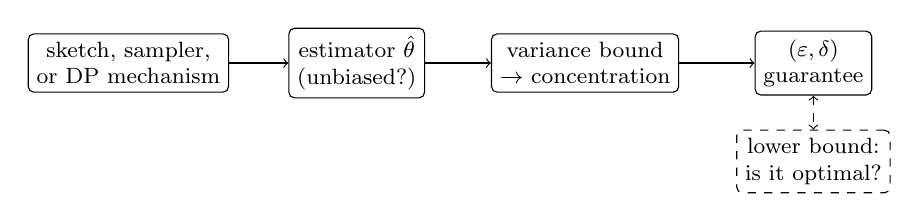
\begin{tikzpicture}[
  box/.style={draw, rounded corners=2pt, inner sep=3pt, align=center, font=\footnotesize}]
\node[box] (s)   at (0,0)    {sketch, sampler,\\ or DP mechanism};
\node[box] (e)   at (2.9,0)  {estimator $\hat\theta$\\ (unbiased?)};
\node[box] (v)   at (5.8,0)  {variance bound\\ $\to$ concentration};
\node[box] (g)   at (8.7,0)  {$(\varepsilon,\delta)$\\ guarantee};
\node[box, dashed] (lb) at (8.7,-1.25) {lower bound:\\ is it optimal?};
\draw[->] (s) -- (e);
\draw[->] (e) -- (v);
\draw[->] (v) -- (g);
\draw[<->, dashed] (g) -- (lb);
\end{tikzpicture}

\smallskip
{\small The estimator pipeline: every exemplar below walks left to right; the strongest also close the loop.}
\end{center}

\section{Exemplars from the SIGMOD'26 corpus}

\subsection{Perfect $\ell_p$ sampling from exponential variables (streaming)}

One-pass streaming algorithms must output a single index $i$ distributed with probability proportional to $|f_j|^p$, the ideal $\ell_p$ sample; the classical difficulty is that the stream must be tracked under this unusual distribution. The paper treats the output index itself as the estimator and bounds its accuracy per coordinate.

\begin{theorem}[Theorem 1 of \cite{sigmod26-247}: $\ell_p$ sampler]
For any constant $p\in(0,2]$, there is a one-pass streaming algorithm that runs in space $\widetilde{O}(\log^{c(p)} n\cdot\log(1/\delta))$ and outputs an index $i$ such that, with probability at least $1-\delta$, for every $j\in[n]$,
\[
\Pr[i=j] \;=\; \frac{|f_j|^p}{\lVert f\rVert_p^p} \;\pm\; \frac{1}{\mathrm{poly}(n)},
\qquad
c(p)=\begin{cases} 1 & 0<p<2,\\ 2 & p=2.\end{cases}
\]
\end{theorem}

\begin{corollary}[Corollary 3.3 of \cite{sigmod26-247}]
Let $f\in\mathbb{R}^n$ be a frequency vector and let $(e_1,\dots,e_n)$ be i.i.d.\ exponential random variables with rate $1$. Define $z_i = f_i/e_i^{1/p}$ and let $(D^{(1)},\dots,D^{(n)})$ be the anti-rank vector of the vector $(z_1^{-p},\dots,z_n^{-p})$. Then
\[
\Pr\big[D^{(1)}=i\big] \;=\; \frac{|f_i|^p}{\lVert f\rVert_p^p}.
\]
\end{corollary}

What is estimated is a whole distribution rather than a scalar, and the error bound is an $\ell_\infty$ bound on the sampled probabilities. The estimator trick is the exponential race: by scaling, $e_i/f_i^p = z_i^{-p}$ is exponential with rate $|f_i|^p$, so the minimum is attained at $i$ with exactly $\ell_p$ probability; the streaming algorithm then only has to track the rescaled vector $z$ (via BPTree, CountSketch, and AMS sketches), repairing the nonlinear $x^p$ step with Taylor-series and geometric-mean estimators, with Chebyshev and union bounds supplying the $\pm 1/\mathrm{poly}(n)$ accuracy. \cite{sigmod26-247}\pods

\subsection{Unbiased Laplace-noised walk counting (local differential privacy on graphs)}

Counting $k$-line walks in a graph where every node privatizes its own view (edge-local DP) forces fresh Laplace noise at each of $k$ synchronous rounds, so the naive error compounds with $k$; the question is how much accuracy a $k$-round message-passing mechanism can retain.

\begin{theorem}[Theorem 4.2 of \cite{sigmod26-012}]
For any graph $G$, walk length $k$, and parameters $\varepsilon$ and $\beta$, the $k$-round mechanism $\mathcal{M}_{k\text{-wk}}$ satisfies $\mathbb{E}[\mathcal{M}_{k\text{-wk}}(G,\varepsilon)] = W_k$, and with probability at least $1-\beta$,
\[
\big|\mathcal{M}_{k\text{-wk}}(G,\varepsilon) - W_k\big|
\;\le\; k\gamma\sqrt{N}\,\big(d(G)+\gamma\big)^{k-1}
\;=\; \widetilde{O}\big(\sqrt{N\, d(G)^{k-1}}\big),
\]
where $\gamma = 2k\sqrt{8\log(2kN/\beta)}/\varepsilon = \widetilde{O}(1)$, with $N$ the number of nodes and $d(G)$ a degree parameter of $G$.
\end{theorem}

What is estimated is $W_k$, the number of $k$-line walks; the bound is unbiasedness plus a high-probability additive error of $\widetilde{O}\big(\sqrt{N\,d(G)^{k-1}}\big)$, improving on the typical $O(N^{k/2})$ of naive Laplace counting. The estimator trick is sensitivity control by induction: each round adds per-node Laplace noise scaled by the running maximum $\lVert X^{(\ell-1)}\rVert_\infty$, a Laplace concentration bound (failure budget $\beta'/N$ per node per round) yields $\lVert X^{(\ell)}\rVert_\infty \le (d(G)+\gamma)^{\ell}$, and union bounds close the loop; a complementary variance lower bound of $\Omega(N^{k+1})$ for the baseline estimator, obtained by summing variances over all oriented $k$-line walks, shows the multi-round design is genuinely needed. \cite{sigmod26-012}

\subsection{Variance recursion and an entropy lower bound for expandable sketches}

A frequency-estimation (FE) sketch for streams of unknown, unbounded length must expand as the stream grows; the paper asks both how accurate such a sketch can be and how much memory the expansion forces, matching the two sides.

\begin{lemma}[Variance of the sketch \cite{sigmod26-231}]
Like CountSketch, the sketch provides unbiased estimates. Moreover, letting $V(F)$ denote its estimation variance when using a size function $W(\cdot)$ and one array on a stream with squared $\ell_2$-norm $F=\sum_y (f(y))^2$, we have at the end of epoch $i$ that
\[
V(F_{i+1}) \;\le\; \frac{1}{W_i}\cdot\sum_{j=0}^{i} 2^{\,i-j}\cdot\big(F_{j+1}-F_j\big),
\]
where $F_j$ denotes the squared $\ell_2$-norm of the stream at the start of epoch $j$.
\end{lemma}

\begin{theorem}[Space lower bound \cite{sigmod26-231}]
Consider an FE sketch with only overestimation errors that processes growing streams with an error bound of $E(N)$ and a confidence of $1-\delta$. Such a sketch must use at least
\[
\frac{N}{E(N)}\cdot\Big[\Omega\Big(\log\tfrac{1}{\delta}+\log\log\tfrac{N}{E(N)}\Big)-\Theta(1)\Big]
\]
bits of memory at some point in time while processing a stream.
\end{theorem}

What is estimated are per-key frequencies, unbiasedly as in CountSketch; the error bound is a variance recursion over geometrically spaced epochs, each past expansion contributing with weight $2^{\,i-j}$, and Markov/Chebyshev convert it into the stated confidence. The complementary trick is the lower bound: an entropy-incompressibility argument (by reduction to filters) shows any sketch achieving error $E(N)$ at confidence $1-\delta$ must pay the displayed bits, and the constructed sketch lands within a small logarithmic factor of it --- the estimation-theoretic ideal of a matched pair. \cite{sigmod26-231}

\subsection{Concentration-chosen sample sizes for influence minimization}

Blocking nodes to curb time-critical misinformation spread requires maximizing a benefit function $D(\cdot)$ that is $\#P$-hard to evaluate and non-submodular, so greedy must run on sampled surrogates; the question is how many samples suffice for the greedy choice to provably transfer to the true objective.

\begin{theorem}[Theorem 6.7 of \cite{sigmod26-373}]
Given $0\le\varepsilon,\delta\le 1$, CBFM returns $B^{*}$ satisfying
\[
\Pr\big[D(B^{*}) \;\ge\; \tau\big(1-\tfrac{1}{e}-\varepsilon\big)\cdot D(B_{o})\big] \;\ge\; 1-3\delta,
\]
where $B_{o}$ denotes an optimal solution.
\end{theorem}

What is estimated is $D(B)$ itself, by an unbiased estimator $\hat D(B)$ built from reverse-score sample sets (GRS/TRS) whose coverage terms are unbiased; the error bound is an end-to-end $(1-1/e-\varepsilon)$-style approximation holding with probability $1-3\delta$, where $\tau$ reflects that greedy optimizes $D$ through the submodular surrogates sandwiching it ($D_L \le D \le D_{U'}$). The estimator trick is to derive the sample threshold analytically: concentration bounds fix the maximal sample size $\theta_{\max}$, and three union-bound events account for the $3\delta$. \cite{sigmod26-373}

\subsection{How many random trees? (biharmonic distance)}

Pairwise biharmonic distance requires quantities from the square of the Laplacian pseudoinverse, which no near-linear graph algorithm computes exactly; the paper reformulates the distance and estimates each term by averaging over randomly sampled spanning trees.

\begin{theorem}[Theorem 6.3 of \cite{sigmod26-102}]
If $\omega_t = d_v^2\Delta^2\log(2n/\delta)/(2\varepsilon^2)$, FastTree samples $\omega_t$ trees, and the corresponding estimators satisfy that for each node $u$,
\[
\big|x_a(u)-\tilde{x}_a(u)\big| \le \varepsilon
\qquad\text{and}\qquad
\big|x_b(u)-\tilde{x}_b(u)\big| \le \varepsilon .
\]
\end{theorem}

What is estimated are the two terms $x_a,x_b$ of the reformulated distance (a pivoted identity rewrites $\beta(s,t)$ via $\widehat L_v^{-1}$ and a rank-structured correction), each by the average of $\omega_t$ unbiased tree-sampling estimators grounded in electrical-network/Kirchhoff identities; the error bound is per-node $\varepsilon$-accuracy from Chernoff--Hoeffding plus a union bound over all $n$ nodes. The trick is visible in the sample count itself: it is exactly the canonical Hoeffding size (range scale $d_v\Delta$, with $d_v$ the pivot degree and $\Delta$ a graph parameter) squared, times $\log(2n/\delta)$, over $2\varepsilon^2$ --- the matrix inverse is replaced by an expectation over absorbing random walks. \cite{sigmod26-102}

\begin{reachbox}{When to reach for estimation theory}
\begin{itemize}
\item You report a number derived from a sketch, a sample, or a randomized mechanism, and must attach error bars or an $(\varepsilon,\delta)$ confidence to it.
\item Unbiasedness is the workhorse: it makes variances add across keys, rounds, or nodes, so one variance bound plus Chebyshev/Chernoff delivers the guarantee.
\item Nonlinearity breaks unbiasedness ($\mathbb{E}[g(X)] \neq g(\mathbb{E}[X])$); fix it with Taylor-series or geometric-mean corrections instead of ignoring the bias.
\item To size a structure, invert the concentration bound: sample counts of the form $\omega \approx \mathrm{range}^2\log(n/\delta)/(2\varepsilon^2)$ should fall out analytically, not be tuned.
\item To certify optimality, pair the upper bound with a variance, Cram\'er--Rao, Le~Cam/Fano, or entropy-incompressibility lower bound; matching within logarithmic factors is the gold standard.
\item Remember the two hidden costs: union bounds charge $\log(\#\text{quantities})$, and minimax bounds rate the estimator class, not your implementation.
\end{itemize}
\end{reachbox}

\chapter{Adversarial Constructions: How Lower Bounds Get Built}

An upper bound is a promise; an impossibility result is the proof that no better promise exists. The second kind of theorem is not derived from the first --- it is \emph{built}. To show that no algorithm, language, or sketch in a model can do better, the author must construct the world in which every allowable procedure fails: a pair of instances, a hard distribution, a stream of updates engineered so that succeeding is impossible and failing is provable. That engineered world is the \emph{adversary}, the workhorse of impossibility. In our corpus the tool is used by 21 of 228 tagged papers, and it owns the survey's signature pairing: 13 of those papers prove an upper bound \emph{and} its matching adversarial lower bound in the same article. The pairing is no accident --- the upper bound tells you what the adversary must force; the adversary certifies that the upper bound is the end of the line.

\section{The Tool: Anatomy of an Adversarial Argument}

Strip away the domain vocabulary and adversarial arguments share a three-part skeleton.

\paragraph{The world: an instance family.}
Fix the model of computation or observation --- the rows of a linear sketch, a stream of tuple inserts and deletes, the syntax of an algebra, a class of colored graphs. Inside that model, design the instance family: often two planted instances $I_0$ and $I_1$, or, via Yao's minimax principle~\cite{adversarial-construction-bg1}, a single hard input distribution against which the best deterministic procedure is analyzed.

\paragraph{Forced behavior or information blindness.}
Argue that \emph{every} procedure in the model is constrained on the family, for one of two reasons. \emph{Information blindness}: the observation available to the algorithm (a sketch, a transcript, a vector of walk counts) simply does not contain the bit that distinguishes the instances. \emph{Forced behavior}: the model's own syntax caps a resource --- e.g.\ an expression of size $\ell$ can multiply tuple multiplicities by at most $2^{\ell}$ --- and the adversary exhibits an instance whose correct answer exceeds every cap.

\paragraph{The two-instance indistinguishability pattern.}
The decisive move: instances $I_0$ and $I_1$ produce identical observations yet demand different answers, so any output is wrong on one of them.

\begin{center}
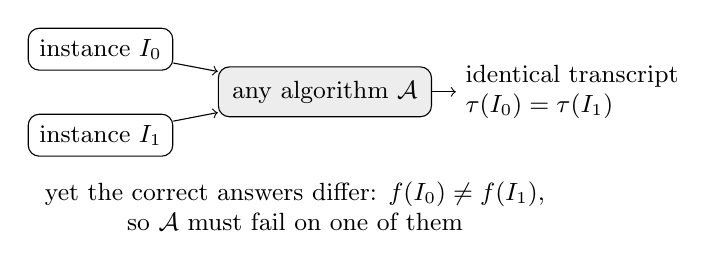
\begin{tikzpicture}[scale=0.95, every node/.style={font=\small}]
  \node[draw, rounded corners, inner sep=4pt] (I0) at (0,1.15) {instance $I_0$};
  \node[draw, rounded corners, inner sep=4pt] (I1) at (0,0) {instance $I_1$};
  \node[draw, rounded corners, inner sep=5pt, fill=black!7] (A) at (3,0.58) {any algorithm $\mathcal{A}$};
  \node[align=left, anchor=west] (T) at (4.75,0.58) {identical transcript\\$\tau(I_0)=\tau(I_1)$};
  \draw[->] (I0) -- (A);
  \draw[->] (I1) -- (A);
  \draw[->] (A) -- (T);
  \node[align=center] at (2.6,-0.95) {yet the correct answers differ: $f(I_0)\neq f(I_1)$,\\ so $\mathcal{A}$ must fail on one of them};
\end{tikzpicture}
\end{center}

\paragraph{Imported adversaries: reductions and communication complexity.}
When no direct planting suffices, the adversary is imported. A conditional lower bound is an adversary-as-reduction: an effective procedure converts instances of a believed-hard problem ($k$-clique, OuMv, SETH) into instances or update sequences of yours, so any fast algorithm would refute the conjecture --- the dominant pattern for dynamic graph and query problems~\cite{adversarial-construction-bg5}. Communication complexity hands out prefabricated two-player adversaries --- index, set-disjointness, gap-Hamming --- whose transcripts are information-blind by construction~\cite{adversarial-construction-bg2}; sketching lower bounds in databases have ridden this route since the frequency-moment bound~\cite{adversarial-construction-bg3}. And when the object under attack is a \emph{language} rather than a cost, the adversary is a witness object, from Moon--Moser's triangle graph~\cite{adversarial-construction-bg4} to the counterexamples that have measured relational completeness since Codd~\cite{adversarial-construction-bg6}.

\section{Exemplars from the Corpus}

\subsection{Walk-Equivalent Graph Pairs and GNN Expressiveness}

MPLang is a matrix-programming language capturing GNN-style computation over embedded graphs; its affine fragment A-MPLang omits activation functions. What can the affine fragment even see?

\begin{corollary}
The following are equivalent for pointed $d$-embedded graphs $(G_1,\gamma_1,v_1)$ and $(G_2,\gamma_2,v_2)$:
\begin{enumerate}
  \item $e(G_1,\gamma_1)(v_1) = e(G_2,\gamma_2)(v_2)$ for every A-MPLang expression $e$ of $A^{+}$-depth $n$ over $d$-embeddings;
  \item $((A^{+})^{i}\,1)(G_1,\gamma_1)(v_1) = ((A^{+})^{i}\,1)(G_2,\gamma_2)(v_2)$ and $((A^{+})^{i}P_j)(G_1,\gamma_1)(v_1) = ((A^{+})^{i}P_j)(G_2,\gamma_2)(v_2)$ for all $i \in [n]$ and $j \in [d]$.
\end{enumerate}
The condition in the second item defines $(G_1,v_1,\gamma_1)$ and $(G_2,v_2,\gamma_2)$ being \emph{$n$-walk equivalent}.
\end{corollary}

A normal-form theorem shows every affine expression of depth $n$ is a fixed polynomial in the walk-count features of item 2, so any two graphs agreeing on those counts are indistinguishable to the entire fragment --- the textbook two-instance pattern, with walk statistics as the shared transcript. A single walk-equivalent pair that disagrees on the target query kills the fragment, and red--blue symmetric trees (with induction on expression shape) extend the witnessing to separate activation-function classes: any $\Sigma$-MPLang expression must stay symmetric exactly where a ReLU threshold can break symmetry. \cite{sigmod26-004}\pods{}

\subsection{Sketching Dimension for $\ell_2$ Sampling}

A linear $\ell_2$-sampling sketch observes $Sv$ and must output coordinate $i$ with probability roughly $v_i^2/\lVert v\rVert_2^2$. How many rows must $S$ have, and how many bits store $Sv$?

\begin{theorem}
An $(\epsilon,\delta)$-$\ell_2$-sampler with frequency estimation requires a sketching dimension of at least $\Omega\bigl(\tfrac{1}{\epsilon}\log^2 n + \tfrac{2}{\epsilon}\log n\bigr)$. Moreover, storing such a sketch for vectors with poly$(n)$-sized entries requires $\Omega\bigl((\log^3 n + \tfrac{2}{\epsilon}\log^2 n)/\epsilon\bigr)$ bits.
\end{theorem}

The adversary is a planted distribution made rigorous by Yao's principle: $m$ short Gaussian spikes sit on isotropic background noise, so each row of the sketch observes a location mixture $X \sim N(v_I, I_d)$ with $I$ uniform and $\lVert v_i\rVert \le 10\ln m$. The paper's Lemma 2 bounds recovery of $I$ from $X$ by $2m^{-1/2}$ --- the spikes are information-blind to any decoder --- and a payout-game argument converts failed identification into sampling error. \cite{sigmod26-241}\pods{}

\subsection{Conditional Lower Bounds for Dynamic Query Maintenance}

A dynamic algorithm maintains the answers to a fixed conjunctive query $Q$ under single-tuple inserts and deletes, with amortized update time and enumeration delay. Which maintenance times are achievable without blowing up the update cost?

\begin{theorem}
Assuming the combinatorial $k$-clique conjecture, no dynamic combinatorial algorithm can maintain $Q$ with amortized update time $O(|D|^{(k-1)/k-\epsilon})$ and support constant-delay enumeration, for any constant $\epsilon > 0$.
\end{theorem}

Here the adversary is imported: a reduction encodes $k$-cycle detection (via color-coding hash families) and OuMv tensor products into an update sequence on the database, so a faster maintenance algorithm would solve the conjecture-hard problem. The reduction \emph{is} the adversary --- it generates the stream adaptively, and indistinguishability is inherited from the source problem rather than planted directly. \cite{sigmod26-244}\pods{}

\subsection{Expressiveness: Relational Algebra Without Division}

On $\mathbb{K}$-databases every tuple carries a semiring value, and the paper asks which fragments of calculus and algebra still coincide in the spirit of Codd's theorem~\cite{adversarial-construction-bg6}. One operation resists every expression.

\begin{theorem}
There is no expression of basic relational algebra $\mathrm{BRA}$ that defines the division operation $\div$ on $\mathbb{N}$-databases.
\end{theorem}

This is forced behavior by a counting ceiling: structural induction shows every $\mathrm{BRA}$ expression $E$ on inputs of size $n$ has support at most $n^{\ell(E)}$ and multiplicities at most $p_E(n)\cdot 2^{\ell(E)}$ --- single-exponential growth in expression size. The adversary is one $2^n$-multiplicity division instance, which outruns the budget of every fixed expression; no pair of instances is needed, only growth rates. \cite{sigmod26-290}

\subsection{Output-Sensitive Witness Graphs for Defective Cliques}

A $k$-defective clique is a vertex set missing at most $k$ edges; enumeration algorithms are judged by search space relative to output. How large must the output itself be in the worst case?

\begin{theorem}
The worst-case output size of maximal $k$-defective clique enumeration is $\Omega(3^{n/3}\cdot n^{k})$ when $k$ is a constant.
\end{theorem}

The adversary is a Moon--Moser-style witness graph~\cite{adversarial-construction-bg4}: disjoint triangles already force an independent three-way choice per block ($3^{n/3}$ maximal cliques), and each of the $k$ units of permitted defect contributes another polynomial factor of choices. The construction bounds \emph{every} enumeration algorithm --- the output itself is that large --- and thereby certifies the paper's worst-case-optimal search space as tight. \cite{sigmod26-306}

\begin{reachbox}{When to Build an Adversary}
\begin{itemize}
  \item You have (or plan) an upper bound and need to certify optimality: aim the adversary at exactly the resource your algorithm touches --- this is the 13-paper pairing, not a coincidence.
  \item The question is ``can \emph{any} method in this model do better'' or ``is this language expressive enough'', not ``is my implementation correct''.
  \item Recipe: fix the observation model; find what all procedures must share (a transcript, a growth ceiling, a symmetry); plant two instances that share it but demand different answers; or import the pair from a conjecture-hard problem via a reduction, or from communication complexity.
  \item Against randomized algorithms, invoke Yao's principle first and design a hard \emph{distribution}; the analysis then runs against deterministic procedures.
  \item If every two-instance attempt fails, take the hint: perhaps the model is sufficient. Try the matching upper bound before fighting the lower bound.
\end{itemize}
\end{reachbox}

\chapter{Differential Privacy Composition}

Among the 26 SIGMOD'26 papers tagged \texttt{privacy-dp}, composition accounting is close to a monoculture: 69\% of them assemble their end-to-end privacy guarantee by composing mechanisms, and the tool \texttt{dp-composition} is used by 18 of the 228 tagged papers overall, its strongest pairing being \texttt{privacy-guarantee} $\times$ \texttt{dp-composition} (16 papers). The arithmetic itself is shifting: the exemplars below still mostly add plain $(\epsilon,\delta)$ budgets, but the frontier results state composition for R\'enyi DP and $f$-DP, where the composed object is a whole divergence curve rather than a pair of scalars.

\section{The tool}

\begin{definition}[Differential privacy]
A randomized mechanism $\mathcal{M}:\mathcal{D}\to\mathcal{R}$ satisfies $(\epsilon,\delta)$-differential privacy if for all neighboring datasets $D\sim D'$ (differing in one record, edge, or node) and all measurable $S\subseteq\mathcal{R}$,
\[
\Pr[\mathcal{M}(D)\in S] \;\le\; e^{\epsilon}\cdot \Pr[\mathcal{M}(D')\in S] + \delta .
\]
With $\delta=0$ the guarantee is \emph{pure} $\epsilon$-DP \citep{dp-composition-bg1}.
\end{definition}

Five primitives, one line each:
\begin{itemize}
  \item \textbf{Sequential composition.} An adaptive sequence of releases with budgets $(\epsilon_i,\delta_i)$ satisfies $(\sum_i \epsilon_i,\ \sum_i \delta_i)$-DP: budgets add \citep{dp-composition-bg1,dp-composition-bg3}.
  \item \textbf{Post-processing immunity.} Any function of an $(\epsilon,\delta)$-DP output that does not touch the raw data is itself $(\epsilon,\delta)$-DP: analysis after the release is free \citep{dp-composition-bg3}.
  \item \textbf{Group privacy.} Datasets at distance $\lambda$ inherit $(\lambda\epsilon,\lambda\delta)$-DP: the guarantee degrades linearly in group size \citep{dp-composition-bg3}.
  \item \textbf{The R\'enyi ladder.} The Gaussian mechanism (noise $\mathcal{N}(0,\sigma^2 I)$, $\ell_2$-sensitivity $\Delta_2$) is $\bigl(\alpha,\ \alpha\Delta_2^2/(2\sigma^2)\bigr)$-RDP for every $\alpha>1$; RDP composes by adding the $\rho(\alpha)$; and $(\alpha,\rho)$-RDP converts to $\bigl(\rho(\alpha)+\log(1/\delta)/(\alpha-1),\ \delta\bigr)$-DP, optimized over $\alpha$ --- the engine behind $O(\epsilon\sqrt{k})$ rather than $k\epsilon$ for $k$ releases \citep{dp-composition-bg2,dp-composition-bg4}. $f$-DP makes the divergence curve itself the composed object \citep{dp-composition-bg5}.
  \item \textbf{Amplification by subsampling.} An $\epsilon$-DP mechanism run on a $p$-rate Poisson subsample satisfies $\log\!\bigl(1+p(e^{\epsilon}-1)\bigr)$-DP: smaller samples buy smaller budgets \citep{dp-composition-bg6}.
\end{itemize}

\section{Exemplars from SIGMOD'26}

\paragraph{Budget ledgers for private cluster explanations.}
The paper privately explains a given clustering by selecting the attribute combination that best accounts for it: top-$k$ candidate selection, then an exponential mechanism over combinations, then per-cluster histograms \cite{sigmod26-298}.

\begin{proposition}[Sequential composition]
Let $\mathcal{M}_1:\mathcal{D}\to\mathcal{R}_1$ and $\mathcal{M}_2:\mathcal{D}\times\mathcal{R}_1\to\mathcal{R}_2$. Suppose $\mathcal{M}_1$ satisfies $\epsilon_1$-DP and, for every $y\in\mathcal{R}_1$, $\mathcal{M}_2(\cdot,y)$ satisfies $\epsilon_2$-DP (as a function of its first input). Define $\mathcal{M}_3:\mathcal{D}\to\mathcal{R}_2$ by $\mathcal{M}_3(D)=\mathcal{M}_2(D,\mathcal{M}_1(D))$. Then $\mathcal{M}_3$ satisfies $(\epsilon_1+\epsilon_2)$-DP.
\end{proposition}

The end-to-end guarantee is the budget sum $\bigl(\epsilon_{\mathrm{CandSet}}+\epsilon_{\mathrm{TopComb}}+\epsilon_{\mathrm{Hist}}\bigr)$-DP, while inside the histogram stage the clusters are disjoint, so per-attribute and per-cluster releases compose \emph{in parallel}, each contributing $\epsilon_{\mathrm{Hist}}/2$ --- pure multiplicative $e^{\epsilon}$ arithmetic, no divergence needed.

\begin{center}
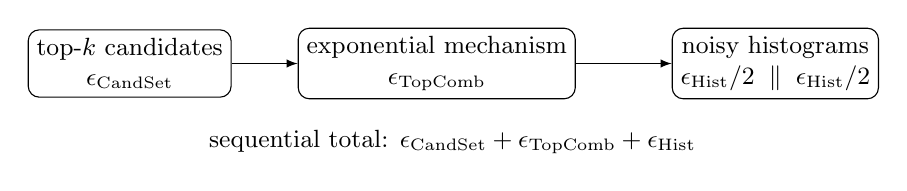
\begin{tikzpicture}[box/.style={draw,rounded corners,align=center,inner sep=3pt,font=\small}]
  \node[box] (a) at (0,0) {top-$k$ candidates\\ $\epsilon_{\mathrm{CandSet}}$};
  \node[box] (b) at (3.9,0) {exponential mechanism\\ $\epsilon_{\mathrm{TopComb}}$};
  \node[box] (c) at (8.2,0) {noisy histograms\\ $\epsilon_{\mathrm{Hist}}/2 \;\parallel\; \epsilon_{\mathrm{Hist}}/2$};
  \draw[-latex] (a) -- (b);
  \draw[-latex] (b) -- (c);
  \node[font=\small] at (4.1,-1.0) {sequential total: $\epsilon_{\mathrm{CandSet}}+\epsilon_{\mathrm{TopComb}}+\epsilon_{\mathrm{Hist}}$};
\end{tikzpicture}
\end{center}

\paragraph{Node-DP from edge-DP via group privacy.}
N2E converts any edge-DP graph mechanism into a node-DP one by clipping the input graph to a degree bound $\Delta^{*}$ that is itself privately approximated, then running the edge mechanism on the clipped graph \cite{sigmod26-337}.

\begin{lemma}[Group privacy]
If a mechanism $\mathcal{M}$ satisfies $(\epsilon,\delta)$-differential privacy, then for any two graphs $G,G'$ with $d(G,G')=\lambda$ (i.e., differing by $\lambda$ edges or nodes) and any subset of outputs $S\subseteq\mathcal{R}$,
\[
\Pr[\mathcal{M}(G)\in S] \;\le\; e^{\lambda\epsilon}\cdot \Pr[\mathcal{M}(G')\in S] + \lambda\delta .
\]
The mechanism satisfies $(\lambda\epsilon,\lambda\delta)$-DP for the group of $\lambda$ edges or nodes.
\end{lemma}

The composition primitive doing the lifting is group privacy: a one-node change is a group of $\lambda$ edge changes, so the edge-DP calculus transfers to node-DP neighborhoods. The degree search spends sparse-vector-technique queries at a logarithmic scale, so only logarithmically many sequential compositions are consumed before post-processing turns the noisy degree into the clipping $\Delta^{*}$; the whole framework satisfies $(\epsilon,\delta)$-node-DP \cite{sigmod26-337}.

\paragraph{Per-record budgets: composition of functions, not scalars.}
Per-record DP replaces the global $\epsilon$ by a budget function $\epsilon_{\mathcal{E}}(r)$ (a bank may assign wealthier clients smaller budgets), and estimates sums/counts by partitioning records into geometrically doubling budget slices, one Laplace mechanism per slice \cite{sigmod26-263}.

\begin{lemma}[PrDP parallel composition]
Let $R_1,\dots,R_k$ be disjoint subdomains and $\mathcal{M}_1,\dots,\mathcal{M}_k$ a series of $\mathcal{E}_i$-PrDP mechanisms. Their parallel composition $\mathcal{M}(D):=\bigl(\mathcal{M}_1(D_{R_1}),\dots,\mathcal{M}_k(D_{R_k})\bigr)$ satisfies $\mathcal{E}'$-PrDP, where $\mathcal{E}'(r)=\max\{\mathcal{E}_i(r)\}_{i=1}^{k}$ for all $r\in[U]^d$.
\end{lemma}

Here the composed object is a budget \emph{function}: releases on disjoint subdomains take a pointwise maximum instead of a sum, so a record is only ever charged the largest budget of any slice touching it. Near-optimality of the resulting error is certified against down-neighborhood lower bounds \cite{sigmod26-263}.

\paragraph{Concurrent composition for continual mechanisms.}
Continual mechanisms answer streams of queries; the hard question is what composition survives an adversary who adaptively and \emph{concurrently} interleaves access to many such mechanisms \cite{sigmod26-049}.

\begin{theorem}[Concurrent composition of continual mechanisms, informal]
The concurrent composition of continual mechanisms $\mathcal{M}_i$ that are $(\epsilon_i,\delta_i)$-DP with respect to a verification function $f_i$ is $(\epsilon,\delta)$-DP for the same $(\epsilon,\delta)$ that holds for composing noninteractive mechanisms that are $(\epsilon_i,\delta_i)$-DP. This allows the adversary to adaptively and concurrently choose the neighboring sequences fed to each $\mathcal{M}_i$ based on the responses received from the other mechanisms.
\end{theorem}

What carries the guarantee is a simulation: every $(\epsilon,\delta)$-DP interactive mechanism can be realized by interactive post-processing of randomized-response outputs, so the divergence arithmetic of ordinary composition transfers verbatim to concurrent adversaries. The same paper pushes the frontier from $(\epsilon,\delta)$ to $f$-DP and R\'enyi DP, complete with a counterexample showing where intuition breaks --- the direction in which the currency is moving. \cite{sigmod26-049}\pods

\paragraph{Composing obliviousness in a multi-way join.}
The differentially oblivious join evaluates queries in untrusted memory while leaking only the input size $|I|$ plus a DP-noisy upper bound $\widehat{OUT}$ on the join size \cite{sigmod26-073}.

\begin{theorem}[Meta-join]
Algorithm~1 is $(\epsilon_1+\epsilon_2,\ \delta_1+\delta_2)$-DO.
\end{theorem}

Two primitives carry it: an $(\epsilon_1,\delta_1)$-DO subroutine releases the $(\epsilon_2,\delta_2)$-DP bound $\widehat{OUT}$, and the advised join's access pattern is a deterministic function of $|I|$ and $\widehat{OUT}$ only. Sequential composition adds both coordinates, and post-processing immunity is precisely what makes an \emph{access pattern} a legitimate object to compose \cite{sigmod26-073}.

\begin{reachbox}{When to reach for DP composition}
Reach for it whenever a system releases \emph{several} interacting statistics and the privacy proof is a ledger: candidate selections, noisy summaries, clipped releases. Then budgets add (exemplars 1 and 5 above, with $\delta$'s summed too in the approximate case), disjoint data slices switch the arithmetic from sums to maxima (exemplars 1 and 3), and group privacy reduces an expensive neighborhood (node-DP) to a cheap one (edge-DP) at linear cost in group size (exemplar 2). Reach for divergence arithmetic --- RDP or $f$-DP curves --- when many releases would make summed $\epsilon$'s vacuous, buying $O(\epsilon\sqrt{k})$ over $k\epsilon$ (the frontier of exemplar 4); reach for subsampling amplification when releases are computed on samples anyway. Post-processing immunity ships every downstream artifact --- clipped graphs, access patterns, indices --- for free. Skip the machinery when a single calibrated release suffices, or when every output is a post-processing of one DP output: composing there only overcounts.
\end{reachbox}

\chapter{Exchange Arguments and Greedy Algorithms}
\setcounter{section}{-1}   % sections start at 7.0 (see main.tex comment)
\label{ch:exc}

\begin{objectives}
\item Recognize when a selection or ordering problem admits an exchange certificate,
  and which structure buys it.
\item Build the exchange: name the partner, count the swap's delta, pick the
  certificate.
\item Match rung to structure: exact (matroid), $1-1/e$ (submodular), $\ln$
  (cover), $3+\varepsilon$ (metric), complete (symmetry).
\item Dissect a paper's greedy: what is committed, what is swapped, what the factor
  is against.
\end{objectives}

A greedy algorithm commits irrevocably: it keeps one plan out of thousands, merges two
chunks, adds one edge to a forest, fixes the order in which an exact search tries
values. The exchange argument is the certificate that makes such myopia safe: it shows
that any solution avoiding the greedy's choice can be \emph{rearranged} --- one
element, edge, or branch swapped for another --- into a solution that honors it, at a
loss that is either zero (the greedy is exactly optimal, or the pruning loses nothing)
or bounded and countable (the greedy keeps a $1-1/e$ or $\ln$ fraction of the optimum).
For a systems paper this converts ``greedy worked well in our experiments'' into a
theorem, and the theory section often shrinks to checking a hypothesis: independence,
diminishing returns, a covering constraint, metric distances, or symmetry. In the
SIGMOD'26 corpus, 17 tagged papers use the tool; in the tag co-occurrences it pairs
with hardness 10 times and with an approximation-ratio property 9 times --- the
signature of ``NP-hard, but structured'' --- and with correctness 7 times, its
exact-rung twin.

This chapter builds the ladder first: the exchange principle, greedy-stays-ahead, the
matroid rung, and the three factor rungs (submodular, set-cover, metric swaps), each
with its swap accounting. Sections~\ref{sec:exc-053}--\ref{sec:exc-009} then dissect
four corpus exemplars at full anatomy; Section~\ref{sec:exc-advanced} adds two
sketched exemplars and further reading.

\section{The tool: exchange arguments and greedy with certificates}
\label{sec:exc-tool}

The problem class is uniform across applications: a solution must be built or selected
incrementally, under constraints, and each increment is irrevocable. The optimizer
keeps a small set of plans, the sampler picks anchors one at a time under a budget,
the temporal index decides edge by edge what a forest remembers, the exact search
commits to a branching order. A greedy algorithm makes each choice by a myopic rule
--- take the plan covering the most workload, the anchor with the best marginal
fidelity, the heaviest edge that keeps a forest, the first value in a fixed order.
What the exchange argument adds is the after-the-fact certificate: a proof that any
solution avoiding the greedy's commitment can be rearranged into one that honors it.
The organizing question of this chapter is which \emph{structure} buys which
\emph{certificate}: independence (matroids) buys exactness, diminishing returns
(submodularity) buys $1-1/e$, covering buys $\ln$, metrics buy $3+\varepsilon$, and
symmetry buys prune-safety --- completeness with no factor at all.

\begin{remarkbox}[Notation]
$U$ is a ground set, $\mathcal{F}\subseteq 2^U$ a feasible family, $w$ (linear
objectives) or $f$ (set functions) the objective to maximize unless said otherwise.
$S_i$ is greedy's set after $i$ picks; $\Delta(u \mid S) = f(S\cup\{u\}) - f(S)$ is
the \emph{marginal gain}; $y$ always names the \emph{exchange partner} --- the
element of the optimal solution that a swap gives up; $O$ denotes an optimal solution
and $\operatorname{OPT}$ its value. $H(n) = \sum_{i=1}^{n} 1/i$ is the harmonic
number. Maximization rungs quote factors $\le 1$ (as $1-1/e$); minimization rungs
quote factors $\ge 1$ (as $H(n)$, $3+\varepsilon$).
\end{remarkbox}

\subsection{The ladder: from exact exchange to logarithmic coverage}
\label{sec:exc-ladder}

The bottom rung is not a theorem about any one problem but the shape of every proof to
come: an optimal solution can be rearranged, one swap at a time, to agree with the
greedy's choices.

\begin{proposition}[Exchange principle]\label{prop:exc-principle}
Let $\mathcal{F}\subseteq 2^U$ be a feasible family and $w\colon\mathcal{F}\to\mathbb{R}$
an objective to maximize. Let $g$ be greedy's first choice, and suppose that for every
feasible $S$ with $g\notin S$ there is an exchange partner $y\in S$ such that
$S' = (S\setminus\{y\})\cup\{g\}$ is feasible with $w(S')\ge w(S)$, and that the same
condition holds recursively on the residual instance with ground set $U\setminus\{g\}$.
Then greedy returns an optimal solution. \eop
\end{proposition}

\begin{proof}
Induction on $|U|$. Let $O$ be optimal. If $g\in O$, then $O\setminus\{g\}$ is optimal
for the residual instance --- any better residual solution would combine with $g$ to
beat $O$ --- and greedy on the residual returns it by hypothesis. If $g\notin O$, the
swap produces an optimal $O' = (O\setminus\{y\})\cup\{g\}$ containing $g$, which
reduces to the first case.
\end{proof}

\begin{figure}[t]
\centering
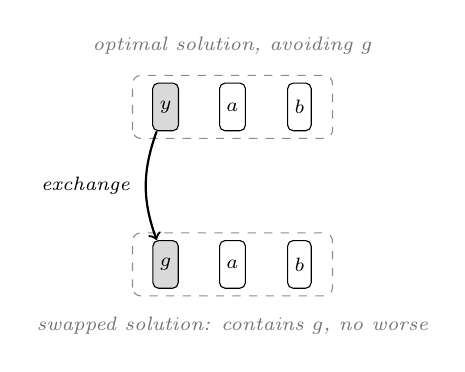
\begin{tikzpicture}[
  every node/.style={font=\scriptsize},
  tok/.style={draw, rounded corners=2pt, inner sep=2.5pt, minimum height=4ex}]
% top row: an optimal solution avoiding g
\node[tok, fill=black!15] (y) at (0,0) {$y$};
\node[tok] (a) at (0.85,0) {$a$};
\node[tok] (b) at (1.7,0) {$b$};
\draw[dashed, rounded corners=3pt, black!45] (-0.42,-0.4) rectangle (2.12,0.4);
\node[text=black!55] at (0.85,0.78) {\itshape optimal solution, avoiding $g$};
% bottom row: the swapped solution
\node[tok, fill=black!15] (g) at (0,-2.0) {$g$};
\node[tok] (a2) at (0.85,-2.0) {$a$};
\node[tok] (b2) at (1.7,-2.0) {$b$};
\draw[dashed, rounded corners=3pt, black!45] (-0.42,-2.4) rectangle (2.12,-1.6);
\node[text=black!55] at (0.85,-2.78) {\itshape swapped solution: contains $g$, no worse};
\draw[->, thick] (y) to[bend right=20]
  node[midway, left=2pt] {\scriptsize\itshape exchange} (g);
\end{tikzpicture}
\caption{The exchange step. Greedy commits to $g$; an optimal solution avoiding $g$
is rearranged into a no-worse solution containing it, one swap at a time. Exact rungs
pay nothing per swap; factor rungs lose a bounded, countable amount that compounds
into the factor.}
\label{fig:exc-swap}
\end{figure}

The next rung makes the rearrangement concrete and shows the craft in miniature: order
the choices well, and the partner swap loses nothing.

\begin{theorem}[Greedy stays ahead]\label{thm:exc-staysahead}
Among all sets of pairwise non-overlapping intervals, the greedy that repeatedly
chooses the compatible interval of \emph{earliest finish time} returns one of maximum
cardinality. \eop
\end{theorem}

\begin{proof}
Write $g_1,g_2,\dots$ for greedy's picks, $o_1,o_2,\dots$ for any optimal solution's,
and $f(\cdot)$ for finish times. By induction, $f(g_i)\le f(o_i)$ for every $i$: it
holds for $i=1$ because greedy takes the earliest-finishing interval of all; and if it
holds for $i$, then $o_{i+1}$ starts at or after $f(o_i)\ge f(g_i)$, so $o_{i+1}$ is
compatible with $g_1,\dots,g_i$ and greedy's $(i{+}1)$-st pick finishes no later than
$o_{i+1}$. Greedy is never behind, so it cannot stop earlier: if the optimum had a
$(k{+}1)$-st interval, it would be compatible with $g_1,\dots,g_k$, and greedy would
have had a choice at step $k{+}1$.
\end{proof}

When the feasibility of each swap is governed by an \emph{independence structure}, the
principle industrializes into an exact algorithm for a whole problem class.

\begin{definition}[Matroid]\label{def:exc-matroid}
A pair $(U,\mathcal{I})$ with $\mathcal{I}\subseteq 2^U$ is a \emph{matroid} if
(i)~$\mathcal{I}$ is hereditary --- $S\in\mathcal{I}$ and $S'\subseteq S$ imply
$S'\in\mathcal{I}$ --- and (ii)~it satisfies the \emph{exchange axiom}: if
$A,B\in\mathcal{I}$ with $|A|<|B|$, then $A\cup\{x\}\in\mathcal{I}$ for some
$x\in B\setminus A$. Members of $\mathcal{I}$ are called \emph{independent} sets.
\end{definition}

\begin{theorem}[Matroid greedy is exact, Edmonds]\label{thm:exc-matroid}
On a matroid, the greedy that scans elements in nonincreasing weight order and keeps
each element that preserves independence returns a maximum-weight independent set ---
for every weight function. Conversely, if greedy is exact for every weight function,
then the family of independent sets satisfies the exchange axiom, so the structure is
a matroid \citep{exchange-greedy-bg1}. \eop
\end{theorem}

\begin{proof}[Proof idea]
The exchange axiom is Proposition~\ref{prop:exc-principle}'s one-for-one swap with
zero loss: if the optimum ``spends'' $y$ where greedy spent $g$ with $w(g)\ge w(y)$,
swap. The full induction is in Section~\ref{sec:exc-appendix}.
\end{proof}

\sidenote{The graphic matroid takes $U$ to be a graph's edges and
$\mathcal{I}$ its forests (acyclic edge sets); maximal independent sets are spanning
forests, and the cycle rule --- an edge that closes a cycle may replace the lightest
edge of that cycle --- is the exchange axiom in the wild. Kruskal's algorithm is the
matroid greedy; the union--find structure that implements it reappears in
Section~\ref{sec:exc-200}.}

Outside matroids exactness dies, but diminishing returns keep a quantitative exchange
alive: greedy's next pick matches the \emph{average} marginal value of the optimum's
remaining elements.

\begin{definition}[Monotone submodular]\label{def:exc-submodular}
$f\colon 2^U\to\mathbb{R}_{\ge 0}$ is \emph{submodular} if
$f(S\cup\{x\}) - f(S) \;\ge\; f(T\cup\{x\}) - f(T)$ whenever $S\subseteq T\subseteq U$
and $x\in U\setminus T$ (diminishing returns), and \emph{monotone} if $S\subseteq T$
implies $f(S)\le f(T)$.
\end{definition}

\begin{theorem}[Submodular greedy, Nemhauser--Wolsey--Fisher]\label{thm:exc-nwf}
Let $f$ be monotone submodular with $f(\emptyset)=0$, and let $A_B$ be the set built
by $B$ greedy steps, each adding the $u\notin A$ that maximizes $\Delta(u\mid A)$.
Then
\[
f(A_B) \;\ge\; \Bigl(1-\frac{1}{e}\Bigr)\max_{|A|\le B} f(A), \eopm
\]
and the factor $1-1/e$ is tight for maximum coverage unless $P=NP$
\citep{exchange-greedy-bg2,exchange-greedy-bg5}.
\end{theorem}

\begin{proof}[Proof idea]
Each greedy pick captures at least a $1/B$ fraction of the remaining optimality gap,
so the gap contracts by $(1-1/B)$ per step; unrolling $B$ steps gives
$(1-1/B)^{B}\le e^{-1}$ (Section~\ref{sec:exc-appendix}).
\end{proof}

When the objective is a covering constraint in disguise --- cover the universe at
minimum total weight --- the same averaging against the optimum yields the harmonic
factor:

\begin{theorem}[Set-cover greedy, Chv\'atal]\label{thm:exc-cover}
Given a universe of $n$ elements and a family of sets with nonnegative weights, the
greedy that repeatedly buys the set maximizing newly-covered elements per unit weight
returns a cover of total weight at most $H(n)\cdot\operatorname{OPT} \le
(1+\ln n)\operatorname{OPT}$, where $H(n)=\sum_{i=1}^{n}1/i$; the bound sharpens to
$H(d)$ when every set has at most $d$ elements \citep{exchange-greedy-bg3}. \eop
\end{theorem}

\begin{proof}[Proof idea]
While $r$ elements remain uncovered, the sets of an optimal cover jointly cover them
at total weight $\operatorname{OPT}$, so one of them covers at rate at least
$r/\operatorname{OPT}$ per unit weight --- and greedy picks at least that well.
Charging each element the price at which it was covered and summing the harmonic
series gives $H(n)$ (Section~\ref{sec:exc-appendix}).
\end{proof}

The last rung replaces ``take the best now'' with ``swap if it helps'': local search
over exchanges, certified by the metric.

\begin{theorem}[Swap local search for $k$-median, Arya et al.]\label{thm:exc-kmedian}
In metric $k$-median, the local search that repeatedly swaps one center for a
non-center whenever it lowers the total assignment cost terminates at a solution of
cost at most $(3+\varepsilon)\operatorname{OPT}$; allowing multi-swaps of up to $p$
centers improves the factor to $2+\varepsilon$ \citep{exchange-greedy-bg4}. \eop
\end{theorem}

\begin{proof}[Proof idea]
At a local optimum no single swap gains. Charge each optimal center to a nearby local
center: the swap that trades one for the other reassigns points through two triangle
inequalities, and the (non-improving) swap's cost delta bounds
$\operatorname{OPT}$ by three times the local cost.
\end{proof}

The rungs share one mechanism --- the swap --- and differ only in the accounting:
\emph{rearrangement} (delta $\ge 0$, greedy optimal), \emph{contraction} (delta $\ge$
gap$/B$, compounding to $e^{-1}$), \emph{averaging} (delta $\ge$
residual$/\operatorname{OPT}$, compounding to $H(n)$), \emph{two triangle
inequalities} ($3+\varepsilon$). Two corpus exemplars below use rungs with no factor
at all: the swap certifies that a construction is exact or that pruning is safe.

\subsection{How to build the exchange}
\label{sec:exc-build}

The construction procedure is mechanical once the greedy rule is written down.
\emph{First}, state what one step commits to --- an element enters the solution, an
edge enters a forest, a value order is fixed. \emph{Second}, take any optimal solution
$O$ that avoids the commitment and \emph{name the exchange partner} $y$: the element
of $O$ doing the job $g$ would do --- the optimal cover's set that greedy's set
displaces, the optimal forest's edge on the cycle $g$ closes, the optimal branch that
tries the values in the other order. \emph{Third}, \emph{count the swap's cost delta}
for $O' = (O\setminus\{y\})\cup\{g\}$: feasibility of $O'$ comes from the structure
(the exchange axiom, heredity, the cycle property, automorphism invariance, plain
coverage), and the delta comes from the objective's arithmetic --- a weight
comparison, a diminishing-returns inequality, a price-per-element average, two
triangle inequalities, or identical neighborhoods. \emph{Fourth}, read off the
certificate type from the delta: zero loss with self-similar residuals gives
exactness; a $1/B$ fraction of the gap gives $1-1/e$; a $1/\operatorname{OPT}$
fraction of the residual gives $\ln$; a strictly earlier branch gives completeness.
The audit effort goes into the \emph{hypothesis}, not the algorithm: submodularity by
pairwise marginal tests or a concave-gain decomposition, the exchange axiom by an
independence oracle, metric structure by the triangle inequality, symmetry by
automorphisms. Near-modular or noisy objectives void the certificate --- and an
honest paper then says so (Section~\ref{sec:exc-advanced}).

\begin{reachbox}{When to Reach for Exchange/Greedy Arguments}
Reach whenever a selection, covering, or clustering problem has been proved NP-hard
(or an exact search explodes) but the objective carries \emph{checkable} structure,
and the deliverable is an algorithm whose quality is a theorem, not a benchmark: a
factor-certified or exactness-certified polynomial-time procedure. Then run the
recipe:
\begin{enumerate}
\item \textbf{Name the exchange partner.} Fix the greedy's next commitment $g$ and an
  optimal solution $O$ avoiding it; identify the element, edge, center, or branch $y$
  of $O$ that plays $g$'s role.
\item \textbf{Identify the structure} that licenses the swap: matroid independence
  (exact), monotone submodularity ($1-1/e$), a covering constraint ($\ln$), metric
  distances ($3+\varepsilon$ swaps), a symmetry group (pruning stays complete).
\item \textbf{Count the swap's cost delta.} Zero loss, a $1/B$ fraction of the gap, a
  $1/\operatorname{OPT}$ fraction of the residual, two triangle inequalities, or
  identical neighborhoods --- the count determines the certificate.
\item \textbf{State the certificate of near-optimality:} which factor, against which
  optimum, with which slack ($\ln\delta^{-1}$, $\varepsilon$) --- inherited, not
  re-derived. If no structure checks out, say so and call the greedy a heuristic.
\end{enumerate}
\end{reachbox}

\section{Risk coresets for robust query optimization}
\label{sec:exc-053}

The exemplar is a PODS'26 paper on robust query optimization \citep{sigmod26-053}\pods.
Query optimizers pick execution plans using cardinality estimates, and the estimates
can be badly wrong; a plan that looks cheapest under the estimates may be terrible on
the true cardinalities. Robust query optimization therefore scores each plan by
\emph{risk}: the probability, over the uncertainty about cardinalities, that the
plan's cost exceeds a factor $\tau$ of the best plan for the realized instance. The
paper asks for a small \emph{coreset} of plans that covers a whole workload
distribution --- after seeing the coreset, a query-time inference step should pick,
from a few precomputed plans, one nearly as robust as the best plan in the entire
exponential space. Its main result is a greedy-cover algorithm that samples
$O((\kappa^{*}/\delta^{2})\ln N\ln(\delta^{-1}))$ queries from the workload and
computes, with high probability, a coreset of size $O(\kappa^{*}\ln\delta^{-1})$ ---
within a logarithmic factor of the smallest coreset $\kappa^{*}$ that exists --- from
which inference returns a plan of risk at most twice the optimum plus $4\varepsilon$.

\paragraph{Problem.}
Work over a plan set $\Pi$ with $|\Pi| = N$ and a workload distribution $W$ over a
query space $\mathcal{Q}$. Each query $Q$ carries an \emph{uncertainty profile}
$U_Q$: a distribution over cardinality vectors $s$, against which plan costs
$\operatorname{Cost}(\pi,s)$ (linear in $s$) are judged. The \emph{penalty} of $\pi$
at $s$ is its cost ratio against the best plan for $s$,
$\operatorname{Pnl}(\pi,s) = \operatorname{Cost}(\pi,s)/\operatorname{Cost}^{*}(s)$,
and the $\tau$-\emph{risk} of $\pi$ on $Q$ is
$\operatorname{Risk}(\pi,Q;\tau) = \Pr_{s\sim U_Q}[\operatorname{Pnl}(\pi,s)>\tau]$,
with $\operatorname{Risk}^{*}(Q;\tau)$ the minimum over all plans. A plan set
$F\subseteq\Pi$ \emph{covers} query $Q$ when its best plan is nearly as robust as the
overall best, $\min_{\pi\in F}\operatorname{Risk}(\pi,Q;\tau) \le
\operatorname{Risk}^{*}(Q;\tau)+\varepsilon$; the failure probability $p(\varepsilon,F)$
is the $W$-probability that $F$ does not cover $Q$, and $F$ is an
$(\varepsilon,\tau,\delta|W)$-\emph{coreset for risk} when $p(\varepsilon,F)\le\delta$.
Let $\kappa^{*}$ be the size of the smallest such coreset. The goal: compute a valid
coreset of size $O(\kappa^{*}\cdot\operatorname{polylog})$ from few workload samples.

\paragraph{Guarantee.}

\begin{theorem}[Risk coreset via greedy cover; Theorem~3.5 of the paper, notation
cleaned]\label{thm:exc-053-main}
Let $W$ be a workload distribution, $\Pi$ a plan set with $|\Pi|=N$, parameters
$\varepsilon\in(0,1]$, $\tau\ge 1$, $\delta\in(0,1)$, and $\kappa^{*}$ the size of the
smallest $(\varepsilon,\tau,\delta|W)$-coreset for risk. For any constants
$c_1,c_2>1$ there is an algorithm that samples
$O\bigl((\kappa^{*}/\delta^{2})\ln N\ln(\delta^{-1})\bigr)$ queries from $W$ and
computes, in time
$O\bigl((\kappa^{*}/(\varepsilon^{2}\delta^{2}))\cdot N\ln^{3}N\cdot
\ln(\delta^{-1})\bigr)$, a set $C\subseteq\Pi$ of size $O(\kappa^{*}\ln(\delta^{-1}))$
such that, with high probability, $C$ is a $(c_1\varepsilon,\tau,c_2\delta|W)$-coreset
for risk. \eop
\end{theorem}

\sidenote{A \emph{coreset} is a small surrogate that preserves the quality of the
full object; here the object is the plan space and the quality is workload-wide risk
coverage. $\kappa^{*}$ is instance-dependent --- small when a few plans already cover
the workload --- which is why the guarantee is stated relative to $\kappa^{*}$ and not
to $N$.}

\paragraph{How the greedy cover is applied.}
The algorithm runs in rounds indexed by a guess $k_r$ that doubles every round; in
round $r$ it samples $\mathfrak{n}_r = (c_1 k_r/\delta^{2})\ln N\ln(\delta^{-1})$
queries from $W$, estimates each plan's risk on each sampled query from
$\mathfrak{m}_r = (c_2/\varepsilon^{2})\ln N\ln\mathfrak{n}_r$ profiles drawn from the
query's uncertainty profile, and runs a maximum-coverage greedy with budget
$b_r = c_3 k_r\ln(\delta^{-1})$ plans: repeatedly add the plan covering the most
not-yet-covered sampled queries, terminating when at least a $(1-2\delta)$-fraction is
covered. Two estimation lemmas make the greedy's proxies faithful: Lemma~3.1 of the
paper bounds the empirical failure probability by Hoeffding plus a union bound over
all $\le (b_r+1)N^{b_r}$ plan subsets of size at most $b_r$, giving
$|\widehat{p}_r(\varepsilon',F) - p(\varepsilon',F)|\le\delta/4$ simultaneously with
probability $1-N^{-O(1)}$; Lemma~3.2 of the paper does the same per (plan, query)
pair, Hoeffding over the $\mathfrak{m}_r$ risk indicators plus a union bound over the
$N\mathfrak{n}_r$ pairs. So the greedy cover behaves almost as if it saw true risks.
The exchange rung --- averaging against the optimal coreset --- is the workhorse:

\begin{lemma}[Greedy termination; Lemma~3.4 of the paper]\label{lem:exc-053-term}
Assuming the conditions of Lemmas 3.1 and 3.2 of the paper hold in every round, the
algorithm terminates with $k_r \le 2\kappa^{*}$. \eop
\end{lemma}

\begin{proof}[Proof sketch]
By Lemma~3.1 the optimal coreset $M$, $|M| = \kappa^{*}$, covers at least a
$(1-5\delta/4)$-fraction $\mathfrak{n}'$ of the sampled queries, so among $M$'s plans
some covers at least a $1/\kappa^{*}$ fraction of whatever residual $D_t$ remains;
greedy picks at least that well, so $D_{t+1}\le(1-1/\kappa^{*})D_t \le
e^{-t/\kappa^{*}}\mathfrak{n}'$. After $t \ge c_3\kappa^{*}\ln(\delta^{-1})$ rounds
the coverage reaches $1-2\delta$, the termination condition --- so the round with
$k_r\ge\kappa^{*}$ terminates, and doubling gives $k_r\le 2\kappa^{*}$. (Full proof in
Section~\ref{sec:exc-appendix}.)
\end{proof}

Deployment adds two transfer steps, both exchange-flavored. Lemma~4.2 of the paper
converts \emph{local} risks (against the coreset $F$) into \emph{global} risks:
\[
\operatorname{Risk}(\pi,Q;\tau^{2}) \;\le\;
\operatorname{L-Risk}_{F}(\pi,Q;\tau) \;+\;
\min_{\pi'\in F}\operatorname{Risk}(\pi',Q;\tau),
\]
so minimizing over $\pi\in F$ bounds the global $\tau^{2}$-risk by twice the best
$\tau$-risk in $F$. Lemma~4.6 of the paper is a Markov step: if $C$ is an
$(\alpha,\delta_1\delta_2|W)$-coreset for neighborhood cost, then the neighborhood
error-rate $N_{\alpha,C}(Q)$ --- the $U_Q$-probability that no plan of $C$ is within
factor $\alpha$ of optimal --- satisfies $\Pr_{Q\sim W}[N_{\alpha,C}(Q)>\delta_1]
\le\delta_2$, because $\mathbb{E}[N_{\alpha,C}(Q)]\le\delta_1\delta_2$ and Markov caps
the tail. Together these give the paper's Theorem~4.1: the inference step, which
scores each coreset plan by its empirical local risk on
$\Theta((\ln|F|+\ln\delta^{-1})/\varepsilon^{2})$ sampled profiles, returns with
probability $1-2\delta$ a plan $\hat{\pi}$ with
$\operatorname{Risk}(\hat{\pi},Q;\tau^{2}) \le 2\operatorname{Risk}^{*}(Q;\tau)+4\varepsilon$.

\paragraph{What it buys.}
The optimizer precomputes once a plan set of size $O(\kappa^{*}\ln\delta^{-1})$ ---
logarithmic slack over the best possible --- and every arriving query is answered by
argmin over that set, in $\Theta(|F|(\ln|F|+\ln\delta^{-1})/\varepsilon^{2})$ time,
with a certified worst-case robustness contract. The greedy cover inherits the
set-cover factor; the Hoeffding and Markov layers only make the cover's input
faithful.

\section{Cohesive subgraphs in temporal graphs, exactly}
\label{sec:exc-200}

The exemplar is a SIGMOD'26 paper on temporal graph queries \citep{sigmod26-200}.
Temporal graphs record when each edge was alive, and analysts routinely ask for
\emph{cohesive subgraphs} --- connected components, $k$-cores, connected $k$-cores ---
restricted to an arbitrary time window: ``the community active between $t_s$ and
$t_e$.'' Answering from scratch per window means recomputing a decomposition for
every query, which is wasteful when windows overlap heavily. The paper instead builds
a single index that answers such \emph{historical} cohesive-subgraph queries for any
window and any of the three models: an \emph{affiliated forest} --- essentially a
Kruskal-style decomposition of the temporal edges, maintained by union--find with
inverse-Ackermann amortization --- plus a compact search structure over the resulting
3-dimensional intervals (BTAS). The headline: $O(m\log m)$ construction, $O(m)$ space,
and $O(n+\log^{2}m)$ per query, exactly, with no approximation anywhere.

\paragraph{Problem.}
A temporal graph $G=(V,E)$ gives each edge a lifespan $[t_1,t_2]$; the snapshot
$G[t_s,t_e]$ keeps exactly the edges whose entire lifespan lies inside the window. A
\emph{cohesive subgraph model} (CSM) $P$ maps each graph to a set of subgraphs;
$P$ is \emph{non-overlapping} when any two subgraphs it returns have disjoint vertex
sets, and \emph{monotonic} when passing to a supergraph only grows the returned
subgraphs. Lemma~2.3 of the paper verifies both properties for the three models of
interest --- the connected component, the $k$-core, and the connected $k$-core (the
$k$-core case itself by a mini exchange argument: two overlapping $k$-cores union to
a larger one, contradicting maximality, so the $k$-core is unique). A
\emph{Historical-CSM} query gives a window $[t_s,t_e]$ and asks for
$P(G[t_s,t_e])$. Each edge becomes a \emph{spanning edge} $(u,v,t_1,t_2)$ of an
affiliated graph, and a lemma of the paper (its Lemma~3.4) reduces Historical-CSM
queries for any non-overlapping, monotonic CSM to a unified, CSM-free
\emph{Spanning-CC} query on the affiliated graph: find all vertex sets that induce
connected components of the windowed affiliated graph.

\paragraph{Guarantee.}

\begin{theorem}[AF-BTAS index; Lemmas 3.6, 3.12, and 3.13 of the paper,
compressed]\label{thm:exc-200-index}
Let $G=(V,E)$ be a temporal graph with $n$ vertices and $m$ edges, and $P$ a
non-overlapping, monotonic CSM. The construction $\mathsf{BuildAF}$ produces, for
every window $[x,y]$, a spanning forest $(V,F_{x,y})$ of the affiliated graph such
that a spanning edge $e=(u,v,t_1,t_2)$ belongs to $F_{x,y}$ if and only if
$0\le x\le t_1$ and $t_2\le y\le\tau(e)$, where $\tau(e)$ is the eviction time
recorded for $e$ (Lemma~3.6 of the paper); the construction is amortized near-linear
through union--find (Lemma~3.8 of the paper). The index AF-BTAS built on the triples
$(t_1,t_2,\tau(e))$ takes $O(m\log m)$ time and $O(m)$ space and answers a Spanning-CC
query for any window in $O(n+\log^{2}m)$ time. \eop
\end{theorem}

\paragraph{How the exchange argument is applied.}
The rung is the graphic matroid: spanning forests are the independent sets, and the
cycle rule --- an edge that closes a cycle may replace a lighter edge of that cycle ---
is the exchange axiom. The paper's $\mathsf{AFDecomp}$ sweeps the spanning edges once,
in an order $\omega_1$ by interval start; a union--find structure maintains the
current forest $S$. When the arriving edge $e_i=(u,v,t_1,t_2)$ connects two vertices
already connected, it closes a cycle: the algorithm finds the $\omega_2$-minimal edge
$e_{\min}$ on that cycle (the one whose usefulness ends earliest) and \emph{exchanges}
--- if $\omega_2(e_i)>\omega_2(e_{\min})$ then $S \gets (S\cup\{e_i\})\setminus\{e_{\min}\}$
and the eviction time is recorded as $\tau(e_{\min}) = t_2-1$; otherwise $e_i$ is
discarded. Every swap is Kruskal's rule applied to a different weight order, and
Lemma~3.6 is precisely the invariant the swaps preserve: an edge survives in exactly
those windows $[x,y]$ that contain its lifespan and end before its eviction. Edges
never evicted get $\tau(e)=t_{\max}$. Correctness of the decomposition is proved by
induction along the sweep (the paper's proof of its Lemma~3.10 shows the running
forest equals each $F_{0,y}$ in turn), and monotonicity of the CSM guarantees
supersets of $u$--$v$ windows stay $u$--$v$ windows (Lemma~3.2 of the paper). The
$\alpha(\cdot)$-amortized union--find checks make the whole sweep near-linear, and the
resulting triples $(t_1,t_2,\tau(e))$ are answered by BTAS --- a binary tree whose
nodes carry priority search trees for the 3-sided query $x\le t_s\le y\le t_e\le z$ ---
in $O(\log m)$ recursion rounds of $O(\log m)$ each plus output size.

\sidenote{The exchange here earns no approximation factor because nothing is
approximated: the cycle swap maintains a \emph{maximum} forest for every window
simultaneously, and the certificate is completeness --- the index answers every query
exactly. This is the matroid rung of Section~\ref{sec:exc-ladder} deployed as a data
structure.}

\paragraph{What it buys.}
One $O(m\log m)$ preprocessing step turns any-window cohesive-subgraph queries into
output-sensitive $O(n+\log^{2}m)$ lookups, replacing per-query recomputation. The same
index serves all three CSMs because the construction uses only non-overlap and
monotonicity, and the union--find amortization keeps the certificate cheap to earn.

\section{Representative sampling for large-scale vector data}
\label{sec:exc-031}

The exemplar is a SIGMOD'26 paper on sampling for vector data \citep{sigmod26-031}.
Graph-based nearest-neighbor indexes navigate a dataset greedily --- beam search hops
from anchor to anchor toward the query --- so everything depends on the anchors being
well placed: globally spread, yet locally dense enough that navigation does not stall.
The paper studies \emph{representative sampling} under a budget: choose a subset of
data points that balances a global coverage constraint against local fidelity, where
fidelity is measured through the local intrinsic dimension (LID) of each point's
neighborhood. It proves the exact selection problem NP-hard, then designs a fidelity
objective $F$ built from per-point gains and shows that (lazy-)greedy under the budget
returns $F$ at least $1-1/e$ of optimal. A companion analysis shows the same anchor
densities that $F$ rewards also make greedy and beam navigation progress with high
probability, via $(1-p)^{m}\le e^{-mp}$ bounds.

\paragraph{Problem.}
Given a dataset of $n$ vectors, a sampling ratio $\rho$ (budget $B=\lfloor n\rho\rfloor$)
and a coverage budget $C_{\max}$, Problem~1 of the paper (\emph{Representative
Sampling}) asks for a sample $A$ of at most $B$ anchors maximizing a local-fidelity
objective $F(A) = \sum_{s} g_s\bigl(m_s(A)\bigr)$ subject to a coverage constraint
$\operatorname{Cost}_{\mathrm{cov}}(A) = \frac1n\sum_{x}\min_{a\in A}
\operatorname{dist}(x,a) \le C_{\max}$, where $m_s(A)$ counts the selected anchors in
point $s$'s neighborhood ball $B(s)$ and $g_s$ is $s$'s per-anchor fidelity gain. The
problem is intractable exactly: Theorem~2 of the paper proves Problem~1 NP-hard by a
parsimonious reduction from metric $k$-median --- set $\rho \gets k/n$ so the budget
forces $|A| = k$, and $C_{\max} \gets T/n$ so the coverage constraint \emph{is} the
$k$-median objective --- so a feasible sample of size $k$ within budget is precisely a
$k$-median answer.

\paragraph{Guarantee.}

\begin{theorem}[Lazy-greedy representative sampling; Theorem~3 of the paper]
\label{thm:exc-031-gre}
Let $B$ be the budget and $A_{\mathrm{gre}}$ the size-$B$ output of the (lazy-)greedy
algorithm (Algorithm~2 of the paper). Then
\[
F(A_{\mathrm{gre}}) \;\ge\; \Bigl(1-\frac{1}{e}\Bigr)\max_{|A|\le B} F(A). \eopm
\]
\end{theorem}

\paragraph{How the submodular greedy is applied.}
The exchange structure is monotone submodularity, and it is earned, not assumed. The
per-point gains come from an estimation analysis: Lemma~1 of the paper represents the
LID estimator at $s$ as $D\cdot(\sum_{j\le m}Y_j)^{-1}$ with $Y_j\sim\mathrm{Exp}(1)$
i.i.d.\ (so $Z=\sum_j Y_j\sim\Gamma(m,1)$), and its gamma-sum moment identities give
closed forms --- mean $D\,m/(m-1)$, variance $D^{2}m^{2}/[(m-1)^{2}(m-2)]$ --- for the
estimator's error at anchor count $m$. Lemma~4 of the paper shows the resulting
mean-squared error $\mathrm{MSE}_s(m)$ is strictly decreasing in $m\ge 3$ with
decrements $\Delta g_s(m) = \mathrm{MSE}_s(m)-\mathrm{MSE}_s(m+1)$ positive and
decreasing, so the cumulative gain $g_s(m)=\sum_{r<m}\Delta g_s(r)$ is nondecreasing
and concave. That concavity is exactly the submodularity hypothesis:

\begin{lemma}[Submodularity of the fidelity objective; Lemma~5 of the paper,
notation cleaned]\label{lem:exc-031-sub}
Let $F(A) = \sum_{s} g_s(m_s(A))$ with each $g_s$ nondecreasing and concave. Then
$F\colon 2^{U}\to\mathbb{R}_{\ge 0}$ is nondecreasing and submodular. \eop
\end{lemma}

\begin{proof}[Proof sketch]
The marginal gain of adding $u$ to $A$ is
$\Delta F(A;u) = \sum_{s\colon u\in B(s)}\bigl[g_s(m_s(A)+1)-g_s(m_s(A))\bigr] \ge 0$,
and if $A\subseteq A'$ then $m_s(A)\le m_s(A')$, so discrete concavity of $g_s$ makes
each bracket at $A'$ no larger than at $A$ --- diminishing returns.
\end{proof}

With Lemma~\ref{lem:exc-031-sub} in hand, Theorem~\ref{thm:exc-031-gre} is the
Nemhauser--Wolsey--Fisher rung (Theorem~\ref{thm:exc-nwf}) verbatim: the greedy pick
captures at least $1/B$ of the remaining gap,
$F(A^{*}) - F(A_i) \le (1-\tfrac1B)\bigl(F(A^{*})-F(A_{i-1})\bigr)$, and unrolling $B$
steps gives $e^{-1}$ (full proof in Section~\ref{sec:exc-appendix}); the lazy
implementation re-evaluates marginals only when stale, preserving the selected
sequence and the factor. Finally, the paper ties the certificate to navigation:
Lemma~3 of the paper bounds the probability that none of $m$ i.i.d.\ neighbors falls
in a spherical cap by $(1-\mu)^{m}\le e^{-m\mu}$, whence its Theorem~1 lower-bounds
the one-layer progress probability by $1-\exp(-\alpha\, m_S(s)\, p_{\mathrm{geom}})$
--- more anchors per region (larger $m_s$, which is what $F$ rewards) means
exponentially smaller stall probability for both greedy ($b=1$) and beam ($b\ge 1$)
expansion.

\paragraph{What it buys.}
A one-page certificate turns a selection problem the reduction just declared hopeless
into a $(1-1/e)$-certified sampler with lazy acceleration, while the coverage
constraint keeps global spread. The moment analysis does double duty: it justifies
the \emph{objective} (why these gains), not just the algorithm, and the
$(1-p)^{m}\le e^{-mp}$ step connects the certified sample to what actually happens at
query time.

\section{Symmetry breaking for maximum common subgraph}
\label{sec:exc-009}

The exemplar is a SIGMOD'26 paper on exact graph matching \citep{sigmod26-009}. The
maximum common induced subgraph (MCIS) problem --- find the largest vertex sets of two
graphs whose induced subgraphs are isomorphic --- is the fundamental model of
structural similarity between graphs, and it is NP-hard. Exact solvers are
branch-and-bound searches that incrementally build vertex correspondences and prune
infeasible or suboptimal branches; on symmetric inputs (regular graphs, repeated
motifs) the search tree explodes into branches that explore the same subproblem over
and over. The paper accelerates the search by detecting \emph{modular symmetry} ---
pairs of vertices with identical neighborhoods --- in $O(n^{2})$ time, and breaking
variable and value symmetries during the search, with proofs that the breaking loses
no solutions. The payoff is exact answers with orders-of-magnitude fewer branches.

\paragraph{Problem.}
MCIS (Definition~2.1 of the paper): given graphs $G$ and $H$, find induced subgraphs
$G[V']$ and $H[U']$ that are isomorphic with $|V'|=|U'|$ maximized. The solver builds
a vertex mapping incrementally; Definition~3.1 of the paper demands two properties of
any acceleration: \emph{correctness} (only mappings between isomorphic induced
subgraphs are deemed valid) and \emph{completeness} (at least one mapping of maximum
cardinality is found). Call vertices $u,v$ \emph{positively symmetric} when their open
neighborhoods coincide, $N^{+}(u)=N^{+}(v)$ (adjacent twins), and \emph{negatively
symmetric} when $N^{-}(u)=N^{-}(v)$ (non-adjacent twins); Theorem~3.1 of the paper
(mutual exclusiveness) shows no vertex can be both. Symmetry \emph{breaking} prunes
branches that try equivalent values in a different order.

\paragraph{Guarantee.}

\begin{lemma}[Modular symmetry is an automorphism; Lemma~1 of the paper]
\label{lem:exc-009-autom}
Two vertices $u,v\in V$ are modular symmetric (positively or negatively) if and only
if the permutation that swaps $u$ and $v$ is an automorphism of $G$. \eop
\end{lemma}

\begin{theorem}[Symmetry breaking is safe; Theorems 3.2 and 3.3 of the paper,
compressed]\label{thm:exc-009-safe}
Variable symmetry breaking and value symmetry breaking do not violate the correctness
or the completeness of the MCIS solution. \eop
\end{theorem}

\paragraph{How the swap argument is applied.}
The greedy commitment is the \emph{fixed branching order}: variables in one fixed
order, values in another. The exchange shows every pruned branch has a symmetric
branch that the search considers strictly earlier. Transcribed from the paper's
proof: suppose a branch $b$ with partial mapping $M$ is pruned because of a conflict
between the correspondence pairs $(v_1,u_2)$ and $(v_2,u_1)$. The swap
\[
(v_1,u_2),\,(v_2,u_1) \;\longmapsto\; (v_1,u_1),\,(v_2,u_2)
\]
creates a symmetric mapping $M'$ on a hypothetical branch $b'$ --- hypothetical
because $b'$ may itself have been pruned. But the search tree branches on all values
of $v$ at the same node in the same fixed order, so $b'$ was considered
\emph{before} $b$; repeated swapping produces earlier and earlier branches, and since
the branch order is well founded, the descent must terminate at a branch the search
actually explores. Every swap preserves cardinality and isomorphism because, by
Lemma~\ref{lem:exc-009-autom}, it is the application of an automorphism --- a
rearrangement of the \emph{same} solution. Hence some maximum mapping survives all
pruning (completeness), and survivors are genuine isomorphisms (correctness). There
is no cost delta to count; the certificate is exactness --- the pruning is free. The
$O(n^{2})$ detection (Lemma~2 of the paper) hashes each vertex's neighborhood, so
finding the exchange partners costs less than using them saves.

\paragraph{What it buys.}
Exact MCIS answers with a fraction of the explored branches, and --- because
Theorem~\ref{thm:exc-009-safe} is a soundness theorem --- the speedup is free: no
approximation is paid for the pruning. The exchange partner is manufactured wholesale
by the automorphism group, turning group symmetry into a completeness certificate for
exact search.

\section{Advanced usage and further reading}
\label{sec:exc-advanced}

Two further corpus papers push the pattern in opposite directions: one runs the
averaging step in weighted form inside an LLM-era retrieval pipeline, the other shows
what an honest paper does when no structure checks out and the greedy carries no
certificate at all.

\paragraph{Skyline retrieval meets set-cover chunk merging \citep{sigmod26-224}.}
Long-context LLM question answering over external documents first retrieves, then
merges, text \emph{chunks} into a compact ``RAG-sketch.'' The paper decomposes queries
into meta-queries, scores chunks on two dimensions (keyword presence and semantic
relevance), takes a skyline per meta-query, and arrives at the merge step: choose a
minimum-token-cost set of chunks covering all meta-queries. Theorem~3.8 of the paper
proves this merge problem NP-hard by a polynomial-time, cost-preserving reduction from
Weighted Set Cover --- treat each chunk as the set of meta-queries it covers, with its
token count as the weight; the forward and backward maps preserve coverage and cost
exactly. The algorithm then merges greedily by gain-per-cost
$G_{t+1}(C) = |Q(C)\cap R_t|/T(C)$ against the residual meta-query set $R_t$, and
Lemma~3.10 of the paper (efficiency) is the averaging step in weighted form: for
every $t$, $G_{t+1}(C_{t+1}) \ge r_t/\operatorname{OPT}$, because an optimal cover's
sets jointly cover the $r_t$ residual meta-queries at total cost
$\operatorname{OPT}$, so one of them covers at that rate --- and greedy picks at least
as well. Unrolling as in Theorem~\ref{thm:exc-cover} gives the logarithmic guarantee,
and an independence argument lower-bounds the expected newly answered queries by
$p_{\min}$ per newly covered meta-query.

\paragraph{Stress-testing causal claims via cardinality repairs \citep{sigmod26-229}.}
Given a causal claim --- an average treatment effect (ATE) of $T$ on $O$ computed over
a database --- the paper asks how fragile it is: find a minimum set of tuples whose
deletion moves the ATE into a target range $[ATE_d-\varepsilon, ATE_d+\varepsilon]$
(or a minimal pattern defining such a subpopulation). The optimization problems are
NP-complete for AVG and ATE aggregates (Propositions of the paper), by a reduction
from SUBSET-SUM: for each number $x$ create tuples $t_x^{1}=(T{=}1,O{=}x)$ and
$t_x^{2}=(T{=}0,O{=}0)$, add one anchor tuple $(1,-k)$, set the target to $0$ ---
deleting exactly the subset of $t_x^{1}$ tuples summing to $k$ zeroes the estimate.
A lemma of the paper shows every tuple set is the extension of some pattern, tying
the pattern variant to the tuple variant. The algorithms (SubCure-tuple,
SubCure-pattern) are then influence-scored greedy heuristics: score each tuple by its
influence $\operatorname{influence}(t) = ATE - ATE_{\setminus\{t\}}$, delete the most
influential, recompute periodically, sample to scale. No approximation factor is
claimed --- influence is not diminishing, submodularity fails, and the paper says so,
verifying the final ATE exactly instead. The contrast with
Sections~\ref{sec:exc-053} and~\ref{sec:exc-031} is the lesson: without checkable
structure, hardness motivates the greedy but certifies nothing.

\subsection{Further reading}

\begin{itemize}
\item Edmonds \citep{exchange-greedy-bg1} --- matroids and the greedy algorithm; the
  exact rung and the exchange axiom, in four pages.
\item Nemhauser, Wolsey, and Fisher \citep{exchange-greedy-bg2} --- the $1-1/e$
  analysis that every submodular corpus paper silently re-runs.
\item Chv\'atal \citep{exchange-greedy-bg3} --- the set-cover charging argument; the
  averaging step in its original home.
\item Arya et al.\ \citep{exchange-greedy-bg4} --- swap-based local search for
  $k$-median and facility location; the canonical metric exchange.
\item Krause and Golovin \citep{exchange-greedy-bg5} --- the survey of submodular
  maximization; lazy greedy, curvature, and non-monotone variants live here.
\end{itemize}

\begin{recap}
\item \textbf{What the tool is.} Exchange arguments certify greedy choices by
  rearranging any better solution to agree with them, one swap at a time: name the
  exchange partner, count the swap's cost delta, inherit the certificate --- exact,
  $1-1/e$, $\ln$, $3+\varepsilon$, or complete.
\item \textbf{Which rung when.} Matroid independence: exact greedy (Kruskal; the
  temporal-forest index of Section~\ref{sec:exc-200}). Monotone submodular under a
  budget: $1-1/e$ (representative sampling, Section~\ref{sec:exc-031}). Covering
  constraint: $\ln$-factor greedy (risk coresets, Section~\ref{sec:exc-053}; chunk
  merging in Section~\ref{sec:exc-advanced}). Metric distances: swap local search at
  $3+\varepsilon$. Symmetry group: pruning stays complete
  (Section~\ref{sec:exc-009}).
\item \textbf{Why it works.} Three swap accountings: rearrangement (delta $\ge 0$,
  greedy optimal), contraction (delta $\ge$ gap$/B$, compounding to $e^{-1}$),
  averaging (delta $\ge$ residual$/\operatorname{OPT}$, compounding to $H(n)$);
  completeness certificates add a well-founded descent --- each pruned branch swaps
  to a strictly earlier one.
\item \textbf{What the corpus showed.} Risk coresets (Section~\ref{sec:exc-053}):
  greedy coverage averaging against the optimal coreset, exponential residual decay,
  $k_r\le 2\kappa^{*}$. Temporal cohesive subgraphs (Section~\ref{sec:exc-200}):
  Kruskal cycle exchanges maintain every window's forest exactly, union--find
  amortized. Representative sampling (Section~\ref{sec:exc-031}): concave-gain
  submodularity plus contraction-unrolling at $1-1/e$. MCIS symmetry breaking
  (Section~\ref{sec:exc-009}): automorphism swaps map pruned branches to earlier
  branches --- pruning certified complete.
\item \textbf{Advanced usage.} Weighted set-cover merging with a per-step averaging
  bound (Section~\ref{sec:exc-advanced}), and an honest certificate-free greedy when
  no structure checks out. Deferred proofs are collected in the Appendix
  (Section~\ref{sec:exc-appendix}).
\end{recap}

\section{Appendix}
\label{sec:exc-appendix}

Proofs omitted from the main text are collected here.

\subsubsection*{Proof of Theorem~\ref{thm:exc-matroid} (matroid greedy)}
{\itshape Statement (recalled).} On a matroid $(U,\mathcal{I})$, the greedy that scans
elements in nonincreasing weight order and keeps each element preserving independence
returns a maximum-weight independent set.\eop

\begin{proof}
Let $G = (g_1,\dots,g_k)$ be greedy's output with weights nonincreasing, and
$O = (o_1,\dots,o_m)$ a maximum-weight independent set, also sorted by nonincreasing
weight. First, all maximal independent sets of a matroid have the same size, so
$k=m$. Second, suppose for contradiction that $w(g_i) < w(o_i)$ for some $i$, and take
the smallest such $i$. The prefix $A = \{g_1,\dots,g_{i-1}\}$ is independent, and so
is $B = \{o_1,\dots,o_i\}$ (heredity), with $|B| = i > |A|$. By the exchange axiom
some $x\in B\setminus A$ has $A\cup\{x\}$ independent, and
$w(x)\ge w(o_i) > w(g_i)$. But then at step $i$ the element $x$ was still available,
kept independence with the prefix, and outweighed $g_i$ --- so greedy would have taken
it. Contradiction. Hence $w(g_i)\ge w(o_i)$ for all $i$, and $w(G)\ge w(O)$. (The
converse --- exactness for every weight function forces the exchange axiom --- is
Edmonds' characterization; see \citep{exchange-greedy-bg1}.)
\end{proof}

\subsubsection*{Proof of Theorem~\ref{thm:exc-nwf} (submodular $1-1/e$)}
{\itshape Statement (recalled).} If $f$ is monotone submodular with $f(\emptyset)=0$
and $A_B$ is greedy's set after $B$ steps, then
$f(A_B)\ge (1-1/e)\max_{|A|\le B}f(A)$.\eop

\begin{proof}
Fix an optimal $A^{*}$ with $|A^{*}|\le B$ and write $A_i$ for greedy's set after $i$
steps. \emph{Fundamental inequality:} adding $A^{*}$'s elements to $A_i$ one at a time
telescopes to $f(A^{*}) - f(A_i) \le \sum_{u\in A^{*}\setminus A_i}
\Delta(u\mid A_i)$, since each marginal along the telescoping is at most the marginal
at the sparser set $A_i$ (submodularity). \emph{Greedy captures the average:} the sum
has at most $B$ terms, each at most the greedy pick's marginal, so
\[
f(A_i) - f(A_{i-1}) \;\ge\; \frac{1}{B}\sum_{u\in A^{*}\setminus A_{i-1}}
\Delta(u\mid A_{i-1}) \;\ge\; \frac{f(A^{*}) - f(A_{i-1})}{B},
\]
which rearranges to the one-step contraction
$f(A^{*})-f(A_i) \le (1-\tfrac1B)\bigl(f(A^{*})-f(A_{i-1})\bigr)$. Unrolling from
$A_0=\emptyset$,
\[
f(A^{*}) - f(A_B) \;\le\; \Bigl(1-\frac1B\Bigr)^{B} f(A^{*}) \;\le\; e^{-1}f(A^{*}),
\]
using $(1-1/B)^{B}\le e^{-1}$. Rearranging gives the theorem.
\end{proof}

\subsubsection*{Proof of Theorem~\ref{thm:exc-cover} (set-cover greedy)}
{\itshape Statement (recalled).} The greedy that repeatedly buys the set maximizing
newly-covered elements per unit weight returns a cover of total weight at most
$H(n)\cdot\operatorname{OPT}$.\eop

\begin{proof}
When greedy buys set $C_t$ at weight $w(C_t)$ covering $d_t$ new elements, charge each
newly covered element $e$ its \emph{price} $\operatorname{price}(e) = w(C_t)/d_t$; the
total weight equals the sum of prices. Let $R_t$ be the residual (uncovered) set
before step $t$, $r_t = |R_t|$. The optimal cover restricted to $R_t$ covers every
residual element at total weight at most $\operatorname{OPT}$, so some optimal set $C$
satisfies $|C\cap R_t|/w(C) \ge r_t/\operatorname{OPT}$; greedy maximizes
newly-covered-per-unit-weight, so its chosen set satisfies it too, and every element
covered at step $t$ pays at most $\operatorname{OPT}/r_t$. Now order all elements
$e_1,\dots,e_n$ by the step at which they were covered. When $e_j$ is covered, at
least $n-j+1$ elements are still uncovered (those covered at or after $e_j$'s step,
including $e_j$), so $\operatorname{price}(e_j) \le
\operatorname{OPT}/(n-j+1)$. Therefore
\[
\sum_{j=1}^{n}\operatorname{price}(e_j) \;\le\;
\operatorname{OPT}\sum_{j=1}^{n}\frac{1}{n-j+1} \;=\; H(n)\cdot\operatorname{OPT}. \qedhere
\]
\end{proof}

\subsubsection*{Proof of Lemma~\ref{lem:exc-053-term} (greedy cover termination)}
{\itshape Statement (recalled).} Under the estimation conditions of Lemmas 3.1 and 3.2
of the paper, the greedy cover terminates with $k_r \le 2\kappa^{*}$.\eop

\begin{proof}
By definition of a coreset there is $M\subseteq\Pi$ with $|M|=\kappa^{*}$ and
$p(\varepsilon,M)\le\delta$. Lemma~3.1 of the paper (with $\varepsilon'=\varepsilon$)
lifts this to the empirical estimate, $\widehat{p}_r(\varepsilon,M) \le
\delta+\delta/4$, so on at least a $(1-5\delta/4)$-fraction of the
$\mathfrak{n}_r$ sampled queries, $\min_{\pi\in M}$ of the proxy risk is within
$2\varepsilon$ of $\operatorname{Risk}^{*}$ (Lemma~3.2 of the paper transfers the
risk estimates): $M$ \emph{covers} at least $\mathfrak{n}' = (1-5\delta/4)\mathfrak{n}_r$
sampled queries under the algorithm's coverage test. Let $D_t = \mathfrak{n}'-|C_t|$
be the residual with respect to the coverable set after $t$ greedy rounds. The
$\kappa^{*}$ plans of $M$ jointly cover $\mathfrak{n}'$ queries, so at round $t+1$ one
of them covers at least $D_t/\kappa^{*}$ of the residual; greedy maximizes marginal
coverage, hence
\[
D_{t+1} \;\le\; \Bigl(1-\frac{1}{\kappa^{*}}\Bigr)D_t \;\le\;
\exp\Bigl(-\frac{t}{\kappa^{*}}\Bigr)\mathfrak{n}'.
\]
For $t \ge c_3\kappa^{*}\ln(\delta^{-1})$ with $c_3$ a suitable constant and
$\delta\le 1/2$, the covered fraction reaches $1-2\delta$, which is exactly the
termination condition --- so the first round with guess $k_r \ge \kappa^{*}$
terminates. Since the guess doubles each round, that round has $k_r \le
2\kappa^{*}$.
\end{proof}

\bibliographystyle{plainnat}
\bibliography{chapters/exchange-greedy-all}

\chapter{Spectral and Matrix-Analytic Arguments}
\setcounter{section}{-1}   % sections start at 8.0 (see main.tex comment)
\label{ch:spec}

\begin{objectives}
\item Recognize when a system's state is a matrix in disguise: transitions, affinities, recursions, Gram matrices.
\item Prove the ladder Rayleigh $\to$ Perron--Frobenius $\to$ Neumann $\to$ interlacing $\to$ low rank/projection.
\item Turn spectral facts into guarantees: rates, invertibility, subspace optimality, distance preservation.
\item Name the matrix, localize the spectrum, exploit the gap or the rank.
\end{objectives}

Spectral and matrix-analytic arguments replace a sprawling object --- a graph,
a recursion, a point set --- with the few numbers that govern its behavior
under repetition: eigenvalues, singular values, spectral radii, eigengaps.
Find the linear map inside the artifact --- a random walk applies a
transition matrix, a smoothness objective is a quadratic form --- then read
the answer off the spectrum: does iteration converge, how fast, and which
subspace carries the object?

In the SIGMOD'26 corpus, 13 papers are tagged with this machinery, pairing it
with graph analytics (spectral clustering of multi-relational graphs, exact
SimRank-style similarity), high-dimensional vector search (subspace
projections and collision counting), and fairness pre-processing through
latent attributes --- plus, a reminder that the tool respects no domain
boundaries, the space utilization of B-tree leaves under batched
insertions. The chapter builds the ladder (Section~\ref{sec:spec-tool}),
dissects four exemplars (Sections~\ref{sec:spec-btree}--\ref{sec:spec-pjsim}), and closes with advanced sketches and further reading
(Section~\ref{sec:spec-advanced}).

\section{The tool: spectral and matrix arguments}
\label{sec:spec-tool}

The problem class is uniform: a square matrix $A$ sits inside the system as
the transition applied by one update step, the quadratic form being
minimized, or the structure behind a vectorized equation; the deliverable
--- limits, solvability, subspaces, distortion --- is decided by where the
eigenvalues of $A$ sit (Figure~\ref{fig:spec-spectrum}).

\begin{remarkbox}[Notation]
$A \in \mathbb{R}^{d \times d}$; for symmetric $A$, eigenvalues $\lambda_1 \ge
\dots \ge \lambda_d$. Operator norm $\|A\|_2$, Frobenius norm $\|A\|_F$,
spectral radius $\rho(A) = \max_i |\lambda_i(A)|$; $A \ge 0$ is entrywise.
$G[A]$: an edge $i \to j$ iff $A_{ij} \ne 0$; $A$ is \emph{irreducible} if
$G[A]$ is strongly connected, \emph{Metzler} if its off-diagonal entries are
nonnegative. $A \otimes B$ is the Kronecker product,
$A \oplus B = (A \otimes I) + (I \otimes B)$ the Kronecker sum,
$\operatorname{Vec}(\cdot)$ stacks columns.
\end{remarkbox}

\subsection{The basic ladder}
\label{sec:spec-ladder}

Eigenvalues are the extreme values of a scalar function of the direction.

\begin{theorem}[Rayleigh quotient]\label{thm:spec-rayleigh}
Let $A = A^{\top} \in \mathbb{R}^{d \times d}$ have eigenvalues $\lambda_1 \ge
\dots \ge \lambda_d$ and orthonormal eigenvectors $v_1,\dots,v_d$. For the
Rayleigh quotient $R(x) = \frac{x^{\top}\!A x}{x^{\top}x}$, $x \ne 0$,
\[
\lambda_1 = \max_{x \ne 0} R(x),
\qquad \lambda_d = \min_{x \ne 0} R(x). \eopm
\]
\end{theorem}

\begin{proof}
$R(x) = \sum_i \lambda_i c_i^2 / \sum_i c_i^2$ for $x = \sum_i c_i v_i$ is a
convex combination of the eigenvalues --- at most $\lambda_1$, at least
$\lambda_d$, with equality at $x = v_1$, $v_d$.
\end{proof}

Most matrices in database papers are not symmetric but \emph{nonnegative} ---
counts, probabilities, affinities --- and there a structure theorem applies
\citep{spectral-matrix-bg1,spectral-matrix-bg5}:

\begin{theorem}[Perron--Frobenius]\label{thm:spec-pf}
Let $A \ge 0$ be irreducible. Then $\rho(A) > 0$ is an eigenvalue of $A$; it
is simple; it admits entrywise positive left and right eigenvectors; and
every other eigenvalue $\lambda \ne \rho(A)$ satisfies
$\operatorname{Re}(\lambda) < \rho(A)$. \eop
\end{theorem}

\begin{proof}[Proof sketch]
Irreducibility makes $A$ eventually map the nonnegative cone into its
interior, so $x \mapsto Ax/\|Ax\|_1$ has an interior simplex fixed point ---
a positive eigenvector for $\rho(A)$; a rank-one positive perturbation shows
the eigenvalue is simple and dominates in real part
\citep{spectral-matrix-bg1}.
\end{proof}

The B-tree exemplar (\citep{sigmod26-038}; Section~\ref{sec:spec-btree}) has
a negative diagonal instead --- a shift by $cI$ fixes that:

\begin{corollary}[Metzler variant, Lemma of \citep{sigmod26-038}, notation
cleaned]\label{cor:spec-metzler}
Let $A$ be an irreducible Metzler matrix admitting an entrywise positive $w$
with $w^{\top}\!A = r\,w^{\top}$, $r > 0$. Then $r$ is a simple eigenvalue
with a positive right eigenvector, and every other eigenvalue $\lambda$
satisfies $\operatorname{Re}(\lambda) < r$. \eop
\end{corollary}

\begin{proof}
$B = A + cI \ge 0$ (with $c = \max_i |A_{ii}|$) is irreducible, and
$w^{\top}\!B = (r+c)\,w^{\top}$ is a positive left eigenvector, which
Perron--Frobenius (Theorem~\ref{thm:spec-pf}) assigns to $\rho(B) = r+c$:
simple, positive right eigenvector, dominant in real part. Since
$\sigma(B) = \sigma(A) + c$, the claims transfer.
\end{proof}

The second rung turns spectral location into a rate: a spectrum strictly
inside the unit disk makes the inverse of $I - A$ a geometric series
\citep{spectral-matrix-bg1}.

\begin{theorem}[Neumann series with truncation rate]\label{thm:spec-neumann}
Let $\rho(A) < 1$. Then $I - A$ is invertible with $(I-A)^{-1} = \sum_{k \ge 0}
A^k$, and for any submultiplicative norm with $\|A\| \le q < 1$ the partial
sum $S_L = \sum_{k=0}^{L} A^k$ obeys
\[
\bigl\|(I-A)^{-1} - S_L\bigr\| \;\le\; \frac{q^{L+1}}{1-q}. \eopm
\]
\end{theorem}

\begin{proof}
$(I-A)S_L = I - A^{L+1}$ and $\|A^{L+1}\| \le q^{L+1} \to 0$; the tail is the
geometric series $\sum_{k > L} q^k$.
\end{proof}

The third rung governs \emph{subspaces}: compressing a symmetric matrix to a
smaller orthonormal basis sandwiches the eigenvalues between those of the
original, making ``which eigenvectors do I keep'' a well-posed optimization
\citep{spectral-matrix-bg1,spectral-matrix-bg2}.

\begin{theorem}[Courant--Fischer and Poincar\'e separation]\label{thm:spec-interlace}
(Courant--Fischer) For symmetric $A$ with eigenvalues $\lambda_1 \ge \dots \ge
\lambda_d$,
\[
\lambda_k(A) \;=\; \min_{\substack{V \subseteq \mathbb{R}^d\\ \dim V = d-k+1}}
\;\max_{0 \ne x \in V} R(x)
\;=\; \max_{\substack{V \subseteq \mathbb{R}^d\\ \dim V = k}}
\;\min_{0 \ne x \in V} R(x).
\]
(Poincar\'e separation) If $B \in \mathbb{R}^{d \times s}$ has orthonormal
columns and $\mu_1 \ge \dots \ge \mu_s$ are the eigenvalues of
$B^{\top}\!A B$, then $\lambda_i(A) \ge \mu_i \ge \lambda_{d-s+i}(A)$,
$i = 1,\dots,s$. \eop
\end{theorem}

\begin{proof}[Proof sketch]
Courant--Fischer: the max--min is attained on the top $k$ eigenvectors' span,
and no $k$-dimensional subspace guarantees more (exchange argument).
Poincar\'e: $B^{\top}\!A B$ is $R$ restricted to $\operatorname{span}(B)$;
Courant--Fischer inside that subfamily sandwiches each $\mu_i$. Full proof
in Section~\ref{sec:spec-appendix}.
\end{proof}

The fourth rung certifies throwing information away: the residual of a
truncated decomposition is governed exactly by the first discarded singular
values \citep{spectral-matrix-bg1,spectral-matrix-bg3,spectral-matrix-bg4}.

\begin{theorem}[Eckart--Young--Mirsky]\label{thm:spec-eym}
Let $A \in \mathbb{R}^{m \times n}$ have singular values $\sigma_1 \ge
\sigma_2 \ge \dots \ge 0$ and singular vectors $u_i, v_i$. Then for every $B$
of rank at most $r$,
\[
\|A - B\|_2 \;\ge\; \sigma_{r+1},
\qquad
\|A - B\|_F \;\ge\; \Bigl(\textstyle\sum_{i > r} \sigma_i^2\Bigr)^{1/2},
\]
and the truncated SVD $A_r = \sum_{i \le r} \sigma_i u_i v_i^{\top}$ attains
both bounds. \eop
\end{theorem}

\begin{proof}[Proof sketch]
$\|A - A_r\| = \sigma_{r+1}$ by inspection of the tail; for the lower bound,
the span of the top $r+1$ right singular vectors meets the kernel of any
rank-$\le r$ $B$, and on a unit $x$ there $\|(A-B)x\|_2 = \|Ax\|_2 \ge
\sigma_{r+1}$. Full proof (both norms) in Section~\ref{sec:spec-appendix}.
\end{proof}

The last rung makes distances cheap: a random low-dimensional projection is
an approximate isometry, with dimension set by accuracy and the number of
events to survive \citep{spectral-matrix-bg3,spectral-matrix-bg4}.

\begin{theorem}[Distributional Johnson--Lindenstrauss]\label{thm:spec-jl}
Let $A \in \mathbb{R}^{d \times D}$ consist of the first $d$ rows of a
uniformly random orthogonal $D \times D$ matrix. Then for every fixed $x \in
\mathbb{R}^D$, $\mathbb{E}\|Ax\|_2^2 = \tfrac{d}{D}\|x\|_2^2$, and for
$\varepsilon, \beta \in (0,1)$ with $d \ge C\,\varepsilon^{-2}\ln(1/\beta)$,
\[
\Pr\Bigl[\;\Bigl|\|Ax\|_2^2 - \tfrac{d}{D}\|x\|_2^2\Bigr| >
\varepsilon\,\tfrac{d}{D}\|x\|_2^2\Bigr] \;\le\; \beta. \eopm
\]
\end{theorem}

\begin{proof}[Proof sketch]
A random orthogonal map takes $x/\|x\|$ to a uniformly random direction, so
$\|Ax\|_2^2/\|x\|_2^2$ is distributed like the squared length of the first $d$
coordinates of a uniform point on the sphere --- approximately $\chi^2_d/d$,
whose concentration gives failure probability $2e^{-\Theta(\varepsilon^2 d)}$;
full proof in Section~\ref{sec:spec-appendix}.
\end{proof}

\begin{widefigure}[t]
\centering
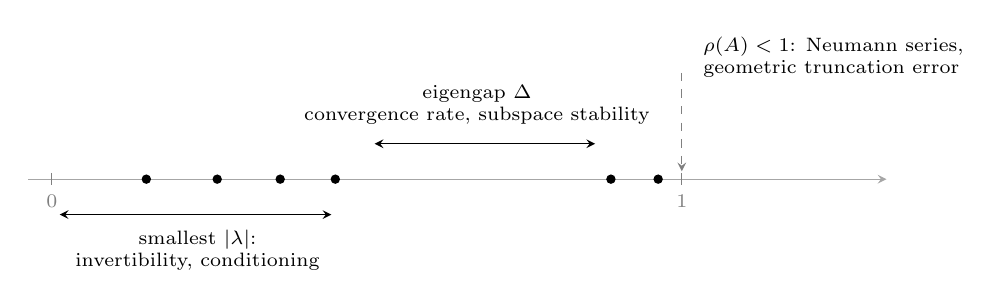
\begin{tikzpicture}[>=stealth]
  \draw[->, gray!70] (-0.3,0) -- (10.6,0);
  \draw[gray] (0,0.08) -- (0,-0.08) node[below, font=\scriptsize, gray] {$0$};
  \draw[gray] (8,0.08) -- (8,-0.08) node[below, font=\scriptsize, gray] {$1$};
  \foreach \x in {1.2, 2.1, 2.9, 3.6, 7.1, 7.7} \fill (\x,0) circle (1.7pt);
  \draw[<->] (4.1,0.45) -- (6.9,0.45);
  \node[font=\scriptsize, align=center] at (5.4,0.95)
    {eigengap $\Delta$\\ convergence rate, subspace stability};
  \draw[<->] (0.1,-0.45) -- (3.55,-0.45);
  \node[font=\scriptsize, align=center] at (1.85,-0.9)
    {smallest $|\lambda|$:\\ invertibility, conditioning};
  \draw[->, gray, dashed] (8,1.35) -- (8,0.1);
  \node[font=\scriptsize, align=left, anchor=west] at (8.15,1.55)
    {$\rho(A) < 1$: Neumann series,\\ geometric truncation error};
\end{tikzpicture}
\caption{Reading a spectrum: distance from $0$ certifies invertibility; a
spectral radius below $1$ licenses a Neumann expansion; a large eigengap
$\Delta$ fixes rates and subspace stability.}
\label{fig:spec-spectrum}
\end{widefigure}

\subsection{How to choose the matrix lens}
\label{sec:spec-choose}

The selection is mechanical. \emph{What are the entries?} Transition counts
or probabilities point at Perron--Frobenius; an optimized quadratic form at
Rayleigh/Courant--Fischer; a huge structured linear system at spectrum
localization plus Neumann; fast-decaying singular values at low-rank
truncation; expensive distances at random projection. \emph{What property is
needed?} Existence needs the spectrum clear of zero; a rate needs a radius
or gap; a subspace recommendation needs interlacing; $(1\pm\varepsilon)$
distances need the JL dimension. \emph{Not symmetric?} Perron--Frobenius, Schur triangularization, or singular values.

\begin{reachbox}{When to Reach for Spectral Arguments}
Reach whenever the object is governed by repetition --- random walks,
recursive similarity, iterative updates, insertion sequences --- or a
combinatorial objective (clustering, subspace selection) hides a quadratic
form. Then run the recipe:
\begin{enumerate}
\item \textbf{Name the matrix}: write down the linear map that one step (one
  batch, one iteration, one hop) applies, and what its entries mean.
\item \textbf{Check the structure}: nonnegative and irreducible $\to$
  Perron--Frobenius (Metzler variant if the diagonal is negative); symmetric
  $\to$ Rayleigh/interlacing; contraction ($\rho < 1$, or eigenvalues in
  $[0,1]$) $\to$ Neumann; fast singular-value decay $\to$ truncated SVD;
  expensive distances $\to$ random projection.
\item \textbf{Localize the spectrum}: row sums, Gershgorin discs,
  stochasticity, or the Kronecker-sum identity $\lambda(A \oplus B) =
  \lambda_i(A) + \lambda_j(B)$ --- place the spectrum relative to $0$ and
  $1$ and bound the dominant gap.
\item \textbf{Convert to the guarantee}: radius $\to$ geometric rate; gap
  $\to$ subspace stability and stopping rule; singular tail $\to$ rank-$r$
  error; projection dimension $\Theta(\varepsilon^{-2}\log(
  \text{events}/\delta))$, union-bounded over all points preserved.
\end{enumerate}
\end{reachbox}

\section{B-tree fragmentation under batched insertions}
\label{sec:spec-btree}

The exemplar is a PODS'26 paper on the space utilization of B-trees
\citep{sigmod26-038}\pods. When a B-tree leaf fills up and splits, the new
leaves start out on average half empty --- underfull leaves mean more cache
misses and rebalancing downstream. Yao's seminal result shows that even
splitting against uniformly random single-key insertions achieves about
$69\%$ space utilization. Many applications, however, insert in
\emph{batches} --- runs of consecutive keys at one position --- a regime
Yao's fringe analysis does not cover. The paper generalizes fringe analysis
to batched workloads: even splitting provably keeps working for many of
them, and simple alternatives cover the remaining regimes.

\paragraph{Problem.}
A B-tree stores keys in leaves (blocks) of capacity $B$. The workload is
random batched insertions: each batch is $r$ consecutive keys inserted at a
uniformly random position, and a \emph{split strategy} decides how an
overflowing block is partitioned. \emph{Fringe analysis} tracks the
histogram of block occupancies --- after $n$ keys, the vector $x^n =
(x^n_k)$ counts blocks of each size $k$ --- and asks for the \emph{expected
final fullness}, the limit of average block size normalized by $B$.

\paragraph{Guarantee.}

\begin{theorem}[Deferred even split fullness, Lemma of \citep{sigmod26-038},
notation cleaned]\label{thm:spec-btree-fullness}
Let $B$ and $i$ be positive integers with batch size $r \in \bigl(B/(2i),\,
B/(2i-1)\bigr]$. Under the deferred even split strategy (a block is split
evenly only when it overflows), the expected final fullness is
\[
\frac{2ir}{B}\,\bigl(H_{2i} - H_i\bigr),
\qquad
H_k = 1 + \tfrac{1}{2} + \dots + \tfrac{1}{k}. \eopm
\]
\end{theorem}

\sidenote{Sanity checks: $r = B$ ($i = 1$) gives fullness $1$; $r = 1$ ($i
\approx B/2$) gives $\approx \ln 2 \approx 0.693$ --- exactly Yao's
classical $69\%$.}

\paragraph{How spectral analysis is applied.}
The named object is the expectation vector $z_n = \mathbb{E}[x^n]$. Since one
batch is linear on the histogram, $z_n$ satisfies an exact \emph{matrix
recurrence}
\[
z_{n+r} \;=\; \Bigl(I + \tfrac{1}{n} A(B,r)\Bigr)\, z_n,
\]
where the $k$-th column of $A(B,r)$ records the net histogram change when a
batch of $r$ keys hits a block of size $k$. $A(B,r)$ is Metzler, and on the
class $S$ of reachable block sizes (a cycle modulo $r$ in the pattern graph)
the principal submatrix $A(B,r)_S$ is irreducible: $w_k = k$ satisfies
$w^{\top}A(B,r)_S = r\,w^{\top}$ (a batch always adds $r$ keys), so
Corollary~\ref{cor:spec-metzler} makes $r$ a simple dominant eigenvalue
with positive eigenvector. Convergence of the recurrence is the workhorse.

\begin{theorem}[Convergence of the matrix recurrence, Theorem of
\citep{sigmod26-038}, notation cleaned]\label{thm:spec-btree-recurrence}
Let $v_{n+r} = \bigl(I + \tfrac{1}{n}A\bigr) v_n$ for $n \ge n_0$, where $r \in
\sigma(A)$ is a simple positive eigenvalue dominating in real part. Then
\[
\lim_{m \to \infty} \frac{v_{n_0 + mr}}{n_0 + mr}
\;=\; P_r^A\Bigl(\frac{v_{n_0}}{n_0}\Bigr),
\]
where $P_r^A$ is the spectral projection onto the generalized eigenspace of
$r$. \eop
\end{theorem}

\begin{proof}[Proof sketch]
Iterating, $v_{n_0+mr} = \bigl(\prod_{k=0}^{m-1} (I +
\frac{1}{n_0+kr}A)\bigr) v_{n_0}$. In Jordan form the mode for $\lambda$
with block size $d$ evolves as scalars $(1 + \lambda/(n_0+kr))$ times a
nilpotent part; the product bound (Lemma~\ref{lem:spec-btree-prod}) shows
the dominant mode grows like $m$, every other like $o(m)$ or $(\ln m)^d$ ---
only the dominant spectral projection survives after division by $m$.
\end{proof}

\begin{lemma}[Scalar product bound, Lemma of \citep{sigmod26-038}, notation
cleaned]\label{lem:spec-btree-prod}
For positive integers $n_0, r$ and $\lambda \in \mathbb{C}$,
\[
\Bigl|\prod_{k=0}^{m-1} \Bigl(1 + \frac{\lambda}{n_0 + kr}\Bigr)\Bigr|
\;\le\; m^{\operatorname{Re}(\lambda)/r}\cdot \alpha_{\lambda, n_0, r},
\]
for a constant $\alpha_{\lambda,n_0,r}$ independent of $m$. \eop
\end{lemma}

\begin{proof}[Proof sketch]
Pointwise $|1+t| \le \exp\!\bigl(\operatorname{Re}(t) + \tfrac{1}{2}|t|^2
\bigr)$; summing over $k$, $\sum_k \operatorname{Re}\bigl(\lambda/(n_0+kr)
\bigr) = \frac{\operatorname{Re}(\lambda)}{r}\ln m + O(1)$ (integral
comparison) and $\sum_k |\lambda|^2/(n_0+kr)^2 = O(1)$. Full proof in
Section~\ref{sec:spec-appendix}.
\end{proof}

The last step is pure \emph{eigenvector arithmetic}. By
Theorem~\ref{thm:spec-btree-recurrence} the normalized histogram converges
into the eigenspace of $r$, and a lemma of the paper pins the limit of the
expected average block size to $\langle u, w\rangle_S / \langle u,
1\rangle_S$ for \emph{any} eigenvector $u$ --- a weighted average over any
partition of $S$, hence at least the minimum class ratio. Three partitions
give three bounds, each favorable in its regime ($r < 0.0058B$, $r < 0.21B$,
$0.21B \le r < 0.5B$), and the eigenvector recurrence $u_k =
\frac{k-r}{k+r}\,u_{k-r}$ (Lemma of the paper) yields the $H_{2i} - H_i$ of
Theorem~\ref{thm:spec-btree-fullness}; the knob $r/B$ selects even, uneven,
or the paper's TargetSplit for long batches.

\paragraph{What it buys.}
The storage engine gets provable utilization numbers per batch-size regime
--- even splitting near-optimal for small $r$, uneven splits above $7/12$ fullness, TargetSplit exact for long batches --- all from one pattern:
recurrence, dominant eigenvalue, product bound, eigenvector arithmetic.

\section{Clustering multi-relational graphs by Dirichlet energy}
\label{sec:spec-mrg}

The exemplar is a SIGMOD'26 paper on clustering large multi-relational graphs
\citep{sigmod26-303}. Multi-relational graphs (MRGs) model objects connected
by many types of interaction at once; partitioning their $N$ nodes into $K$
clusters is a fundamental analytics task. Existing solutions either fuse
the heterogeneous relations so crudely that result quality collapses, or
lean on heavyweight deep models that cannot scale to billions of edges. The
paper proposes DEMM and its scalable sibling DEMM+: first derive node
feature vectors by minimizing a \emph{multi-relational Dirichlet energy}
(a smoothness functional over all relations), then cluster by minimizing
Dirichlet energy over the resulting affinity graph --- DEMM+ never
materializes the dense $N \times N$ matrix and runs in linear time. The
spectral content is threefold: a Neumann series computes the smoothed
embedding, Courant--Fischer-type bounds certify the series is legal, and a
Sinkhorn balancing makes the final step equivalent to plain $k$-means.

\paragraph{Problem.}
Let $G$ be an MRG with $N$ nodes and $R$ relation types; relation $r$ induces
a symmetric normalized affinity $S^{(r)}$, and $S = \sum_{r=1}^{R} \omega_r
S^{(r)}$ with $\sum_r \omega_r = 1$ is the fused affinity. The clustering
objective is a normalized-cut-type quantity over node-cluster incidence
matrices $Y$, equivalent to trace maximization $\max_Y
\operatorname{trace}(Y^{\top}\!SY)$ under combinatorial constraints ---
NP-hard, and it needs the dense matrix $S$. Stage one replaces hard
clustering by continuous features $Z$: minimize $\alpha\,
\operatorname{trace}\bigl(Z^{\top}(I - S)Z\bigr) + \|Z - Z^0\|_F^2$ for
smoothing parameter $\alpha > 0$ and input features $Z^0$.

\paragraph{Guarantee.}

\begin{theorem}[Doubly stochastic affinity gives $k$-means, Theorem of
\citep{sigmod26-303}, notation cleaned]\label{thm:spec-mrg-kmeans}
If the affinity $S_\omega$ is doubly stochastic (all row and column sums
equal $1$) and $Z = Y^{\top}$ is the relaxed embedding, then optimizing the
relaxed trace objective is equivalent to optimizing the $k$-means objective
\[
\min_{C_1,\dots,C_K}\ \sum_{k=1}^{K} \sum_{v_i \in C_k}
\bigl\| z_i - c^{(k)} \bigr\|_2^2,
\qquad
c^{(k)} = \frac{1}{|C_k|} \sum_{v_j \in C_k} y_j ,
\]
where $c^{(k)}$ is the center of cluster $C_k$. \eop
\end{theorem}

\paragraph{How spectral analysis is applied.}
Three matrices are named in turn. \emph{(i) The fused affinity $S$.} Setting
the derivative of stage one to zero gives the closed form $Z =
\frac{1}{1+\alpha}\bigl(I - \frac{\alpha}{1+\alpha} S\bigr)^{-1} Z^0$
(Lemma of the paper) --- an inverse that exists and expands as a Neumann
series (Theorem~\ref{thm:spec-neumann}) because the spectrum of $S$ is
confined to $[0,1]$: a lemma of the paper proves $\lambda(S^{(r)}) \le 1$
by Courant--Fischer (via $\sum_{ij} S_{ij} y_i y_j \le \frac{1}{2}
\sum_{ij} S_{ij}(y_i^2 + y_j^2)$), and the Lidskii-type inequality
$\lambda_{\max}(A + B) \le \lambda_{\max}(A) + \lambda_{\max}(B)$ lifts
through the convex combination. \emph{(ii) The truncated series.}
Truncating at $L$ terms gives the scalable solver:

\begin{lemma}[Truncation error, Theorem of \citep{sigmod26-303}, notation
cleaned]\label{lem:spec-mrg-trunc}
Let $Z^L$ be the $L$-term truncation of the Neumann expansion of
$\frac{1}{1+\alpha}\bigl(I - \frac{\alpha}{1+\alpha}S\bigr)^{-1} Z^0$. Then
\begin{gather*}
\|Z - Z^L\|_F \;\le\;
\Bigl(\frac{\alpha}{1+\alpha}\Bigr)^{\!L+1} \|Z^0\|_F \cdot \max_{j \ge 1}
\mu_{L, L+j},\\
\mu_{\ell_1, \ell_2} = \max_i \bigl|\lambda_i(S)^{\ell_1} -
\lambda_i(S)^{\ell_2}\bigr|,
\end{gather*}
so the error decays geometrically at rate $\alpha/(1+\alpha)$, modulated by
the eigengap quantity $\mu$ --- itself decaying since $\lambda_i(S) \in [0,1]$
($\|S^{L+j} - S^L\|_2 = \mu_{L,L+j}$ exactly). \eop
\end{lemma}

\begin{proof}[Proof sketch]
The tail is $\frac{1}{1+\alpha}\sum_{j \ge 1}
(\frac{\alpha}{1+\alpha})^{L+j}(S^{L+j} - S^L) Z^0$; bound the Frobenius
norm by $\|S^{L+j} - S^L\|_2 = \mu_{L,L+j}$ (read off the eigendecomposition
of $S$), then sum the geometric series in $\alpha/(1+\alpha) < 1$.
\end{proof}

\emph{(iii) The balanced affinity.} The hypothesis of
Theorem~\ref{thm:spec-mrg-kmeans} is manufactured, not assumed:
Sinkhorn--Knopp proportional fitting on $S S^{\top}$ (alternating row and
column normalizations) yields, by Sinkhorn's theorem plus the symmetry of
$S S^{\top}$, a \emph{symmetric doubly stochastic} $S_\omega$ (Theorem of
the paper). And the norms are never computed on $N \times N$ matrices: a
CountSketch (the heavy-hitter hash of the concentration chapter) returns
$\|P S^{(r)}\|_F^2$ to a $(1 \pm \varepsilon)$ factor with probability $1 -
\delta$ using $m = O\bigl(r\varepsilon^{-4}\log(r/\varepsilon\delta)\,(r +
\log(1/\varepsilon\delta))\bigr)$ columns (Corollary of the paper), with
per-relation failure $\delta/R$ union-bounded over the $R$ relations.

\paragraph{What it buys.}
The system clusters billion-edge multi-relational graphs in linear time without ever forming the dense affinity: a truncated Neumann embedding with
certified geometric error, a balancing step with a uniqueness proof, and a theorem chain (spectrum in $[0,1]$ $\to$ Neumann legal $\to$ truncation
rate $\to$ doubly stochastic $\to$ $k$-means).

\section{Subspace collision for high-dimensional nearest neighbor search}
\label{sec:spec-taco}

The exemplar is a SIGMOD'26 paper on approximate nearest neighbor search
\citep{sigmod26-235}. ANNS in high-dimensional Euclidean space is a workhorse
of vector databases, and \emph{subspace collision} is a recently proposed
framework for it: project the data onto many random low-dimensional
subspaces and rank points by how often they ``collide'' with the query ---
fall within its projected neighborhood --- across the subspaces. The
framework performs well but is data-agnostic and query-oblivious, leading to
imbalanced indexes and wasted probing. The paper's system, TaCo, fixes both:
a subspace-oriented data transformation equalizes the subspaces (balanced
average entropy), making collision counting data-adaptive, with query-aware
probing on top. Under the hood, index design is an eigenvalue allocation
problem solved by interlacing, and query-side correctness is projection
non-expansiveness plus Chernoff.

\paragraph{Problem.}
Given a dataset $\mathcal{D}$ of $n$ points in $\mathbb{R}^d$, a query $q$,
and integers $k, N_s, s$ with $N_s \cdot s \le d$: sample $N_s$ subspaces of
dimension $s$; a point $o$ \emph{collides} with $q$ in a subspace if the
projected $o^{\star}$ is among the $(\alpha n)$ nearest neighbors of the
projected $q^{\star}$ there; the SC-score of $o$ counts the subspaces in
which it collides, and the $k$ highest SC-scores are the answer. Two things
must be certified: the \emph{index-side} choice of which dimensions to
group (TaCo first applies an orthogonal transformation $B$), and the
\emph{query-side} fact that projected proximity reflects true proximity.

\paragraph{Guarantee.}

\begin{theorem}[Ordering preservation, Lemma and Theorem of
\citep{sigmod26-235}, merged and notation cleaned]\label{thm:spec-taco-order}
Let $B \in \mathbb{R}^{d \times (N_s \cdot s)}$, $N_s \cdot s \le d$, have
orthonormal columns, so that $BB^{\top}$ is an orthogonal projection.
Suppose that for some $\varepsilon \in (0,1)$ the local difference vectors
satisfy $\|(I_d - BB^{\top})(o_i - o_j)\|^2 \le \varepsilon \|o_i - o_j\|^2$
for all neighbors $o_j$ of each $o_i \in \mathcal{D}$. Then
\[
(1 - \varepsilon)\,\|o_i - o_j\|^2 \;\le\; \|B^{\top}(o_i - o_j)\|^2 \;\le\;
\|o_i - o_j\|^2,
\]
and consequently whenever $\|o_i - o_j\|^2 < (1-\varepsilon)\|o_i -
o_z\|^2$, the relative ordering survives the transformation:
$\|B^{\top}(o_i - o_j)\| < \|B^{\top}(o_i - o_z)\|$. \eop
\end{theorem}

\begin{proof}[Proof sketch]
Pythagoras: $\|o_i - o_j\|^2 = \|B^{\top}(o_i - o_j)\|^2 + \|(I -
BB^{\top})(o_i-o_j)\|^2$; the hypothesis bounds the second term (lower
bound), and projections are non-expansive (upper bound). Chain the bounds
across $o_j$ and $o_z$ for the ordering claim.
\end{proof}

\paragraph{How spectral analysis is applied.}
The named matrix is the sample covariance $\Sigma$ of the transformed data:
$B$'s columns are eigenvectors of $\Sigma$, which is why $BB^{\top}$ is an
orthogonal projection and Theorem~\ref{thm:spec-taco-order} applies. The
index-side question --- \emph{which} eigenvectors to allocate to which
subspace --- is settled by the interlacing rung:

\begin{theorem}[Eigensystem allocation is optimal, Theorem of
\citep{sigmod26-235}, notation cleaned]\label{thm:spec-taco-alloc}
Assume the sample covariance $\Sigma$ has distinct eigenvalues, all $\ge 1$.
Then the Eigensystem Allocation method (assigning eigenvectors of $\Sigma$
to the $N_s$ subspaces so that the subspace log-determinants
$\log\det(B_j^{\top}\Sigma B_j)$ are balanced) solves the paper's balanced
log-det optimization over all choices of the $B_j$. \eop
\end{theorem}

\begin{proof}[Proof sketch]
By Poincar\'e separation (Theorem~\ref{thm:spec-interlace}), the eigenvalues
of each compression $B_j^{\top}\Sigma B_j$ interlace those of $\Sigma$:
$\lambda_i \ge \mu_i \ge \lambda_{d-s+i}$. Since $\log$ is monotone,
maximizing the log-determinant means maximizing the product of compressed
eigenvalues, and interlacing caps each factor at the corresponding top
eigenvalue of $\Sigma$ --- a cap attained by taking $B_j$'s columns to be
eigenvectors; a greedy pass solves the outer balanced partition.
\end{proof}

On the query side, the SC-score is a binomial count: per-subspace collision
probabilities $p^*$ (true neighbor) versus $p < p^*$ (non-neighbor), and the
paper's SC-score Separation lemma shows the optimal Type-I/Type-II errors of
any decision rule decay at rate $\exp\bigl(-N_s\,\Delta(q)^2/(8p(1-p))
\bigr)$, $\Delta(q) = p^* - p$ --- a Chernoff bound on the two binomials.
The tunables: $N_s$ sets the exponent, $\alpha$ moves $p^*$ and $p$ apart,
and $\varepsilon$ is the residual energy the eigensystem leaves outside $B$.

\paragraph{What it buys.}
The vector-search engine gets an index whose subspaces are provably balanced
(equal average entropy, no wasted probing), a certificate that projected-
space comparisons preserve neighbor orderings, and separation growing
exponentially in the number of subspaces.

\section{Exact graph similarity by Kronecker-sum inversion}
\label{sec:spec-pjsim}

The exemplar is a SIGMOD'26 paper on graph similarity
\citep{sigmod26-190}. Quantifying node-to-node similarity is central to
graph analysis, and SimRank is its most-used recursive measure: two nodes
are similar if they are referenced by similar nodes. The classical
definition, however, only counts \emph{equal-length} meeting paths,
producing the ``zero-similarity'' problem --- structurally related nodes
score exactly zero when no symmetric in-neighbor paths exist. Existing
fixes iterate path expansions and pay for expensive convergence checks. The
paper proposes PJsim, an exact, closed-form measure summing meeting paths
of all (possibly unequal) lengths, obtained by reformulating the recursion
as a Sylvester matrix equation solved through structured decompositions;
experiments report higher accuracy than iterative alternatives and speedups
up to $3.22\times$ on synthetic and $2.15\times$ on real graphs. Every
step is an eigenvalue-location argument.

\paragraph{Problem.}
Let $Q$ be the backward transition matrix of a directed graph on $n$ nodes
and $c \in (0,1)$ a decay factor. The PJsim similarity matrix
$S^{\mathrm{PJ}}$ sums contributions over all pairs of meeting path lengths,
which the paper derives to be the solution of the Sylvester equation
\[
X\,S^{\mathrm{PJ}} + S^{\mathrm{PJ}} X^{\top} = 2(1-c)\,I_n,
\qquad X = I_n - c\,Q .
\]
The task: certify a unique solution, then compute it at scale --- the
vectorized system is $n^2 \times n^2$, and naive inversion costs $O(n^6)$.

\paragraph{Guarantee.}

\begin{theorem}[Vectorized solution, Theorem~3.1 and Corollary~3.1 of
\citep{sigmod26-190}, notation cleaned]\label{thm:spec-pjsim-closed}
The PJsim Sylvester equation is equivalent, under the vectorization identity
$\operatorname{Vec}(ABC) = (C^{\top}\!\otimes A)\operatorname{Vec}(B)$, to
the Kronecker-sum linear system
\[
(X \oplus X)\,\operatorname{Vec}\bigl(S^{\mathrm{PJ}}\bigr)
\;=\; 2(1-c)\operatorname{Vec}(I_n),
\qquad X \oplus X = (X \otimes I_n) + (I_n \otimes X),
\]
whose closed-form solution is $\operatorname{Vec}(S^{\mathrm{PJ}}) =
2(1-c)\,(X \oplus X)^{-1}\operatorname{Vec}(I_n)$; the inverse exists. \eop
\end{theorem}

\paragraph{How spectral analysis is applied.}
The named matrix is the Kronecker sum $X \oplus X$ --- the $n^2 \times n^2$
matrix hiding behind the two-sided recursion --- and the rung is spectrum
localization:

\begin{lemma}[Spectrum of the Kronecker sum, Lemma of \citep{sigmod26-190},
notation cleaned]\label{lem:spec-pjsim-spectrum}
The eigenvalues of $X = I_n - cQ$ lie in $[1-c,\, 1]$, and the eigenvalues
of $X \oplus X$ are exactly the pairwise sums $\{\lambda_i(X) +
\lambda_j(X) : i,j = 1,\dots,n\} \subseteq [2(1-c),\, 2]$. Since $c \in
(0,1)$, all eigenvalues of $X \oplus X$ are strictly positive, and $X \oplus
X$ is invertible. \eop
\end{lemma}

\begin{proof}[Proof sketch]
The eigenvalues of the backward transition matrix $Q$ lie in $[0,1]$, so
$\lambda_i(X) = 1 - c\,\lambda_i(Q) \in [1-c, 1]$; the Kronecker-sum
spectrum is the pairwise sum of the summands' spectra ($v_i \otimes v_j$
is an eigenvector of $A \oplus B$ for $\lambda_i(A) + \lambda_j(B)$),
giving $[2(1-c), 2] \subset (0,\infty)$.
\end{proof}

Two consequences follow. \emph{(i) Iterative approximation:} the spectrum
of $I - (X \oplus X)$ lies within the unit disk (the paper expands $(X
\oplus X)^{-1} = \sum_k \bigl[I_{n^2} - (X \oplus X)\bigr]^k$), so the
Neumann rung (Theorem~\ref{thm:spec-neumann}) yields a truncatable,
geometrically convergent series --- an anytime solver with no convergence
checks. \emph{(ii) Exact computation at scale:} apply the real Schur
decomposition $X = VUV^{\top}$ ($V$ orthogonal, $U$ quasi-upper-triangular
with $1 \times 1$ and $2 \times 2$ blocks, real even for complex
eigenvalues). Substituting $Y = V^{\top}S^{\mathrm{PJ}}V$ gives $UY +
YU^{\top} = 2(1-c)I_n$, solved by block back-substitution: the trailing
block a smaller Sylvester equation, the off-diagonal blocks plain linear
systems, each $2 \times 2$ block one $4 \times 4$ inversion --- trivial
against $O(n^6)$. The accuracy knob is the truncation length $K$; the
Schur route is exact.

\paragraph{What it buys.}
The graph-analytics engine gets a similarity measure with no zero-similarity blind spots, an existence proof costing three lines of eigenvalue
arithmetic, and an exact solver --- Schur plus back-substitution instead of $O(n^6)$ inversion --- yielding measured $2$--$3\times$ speedups with
higher accuracy than iterative predecessors.

\section{Advanced usage and further reading}
\label{sec:spec-advanced}

The four exemplars above use spectra of ordinary matrices. Two harder
corpus papers push the same philosophy into tensor decompositions and
random projections; each is sketched in one paragraph.

\paragraph{Fair pre-processing with latent attributes \citep{sigmod26-101}.}
Fair pre-processing calibrates a dataset to a fairness policy so that
sensitive attributes influence outcomes only through designated legitimate
causal pathways --- but real attribute spaces are imperfect:
decision-relevant factors may be inadmissible or simply missing. LatentPre
augments the policy with \emph{latent} attributes and proves the
augmentation recoverable: with one latent attribute and the observed
attributes in four groups (conditional on $(X_0, X_4)$ the first three are
mutually independent), the local parameters of every $X_i$ are
\emph{generically identifiable up to a global permutation of the latent
states} (theorem of the paper). The core: conditioning on each value
$X_4 = j$ yields a three-view latent-class model whose joint distributions
form a $3$-way tensor of low rank $\kappa$ (the number of latent states),
and low-rank tensor decompositions are generically unique --- the
eigenvalues pin down the object. All slices share the same mixing
distribution, so the per-slice permutations must agree, forcing one
consistent global solution; estimation runs by a tailored EM with a
Jensen-bound objective.

\paragraph{Skipping redundant distance computations \citep{sigmod26-265}.}
In graph-based ANN search the distance comparison operation (DCO) ---
compute $\delta(x,q)$, compare against a dynamic threshold $\tau$ --- is
the bottleneck once SIMD makes full distance computations cheap.
SkipComputing replaces the test by a projected-space screen: with $A \in
\mathbb{R}^{d \times D}$ the first $d$ rows of a random orthogonal matrix,
Theorem~4.1 of the paper gives the two-probability contract
$\Pr[\|A(p-q)\|_2^2 < (1+\varepsilon)\tfrac{d}{D}\tau] > p_1$ when
$\delta(p,q) < \tau$, and $< p_2$ when $\delta(p,q) > \tau$ --- the
Johnson--Lindenstrauss rung (Theorem~\ref{thm:spec-jl}) turning the
threshold test into a cheap $d$-dimensional comparison at $d =
\Theta(\varepsilon^{-2}\log(1/\beta))$. Survivors get lower-bound pruning
(MS-distance: a monotone family of lower bounds refining to the exact
distance), and the structure survives PCA pre-processing (Theorem~5.1)
because the PCA rotation is orthogonal, hence norm-preserving.

\subsection{Further reading}

\begin{itemize}
\item Horn and Johnson \citep{spectral-matrix-bg1} --- the comprehensive
  reference: Perron--Frobenius, Kronecker calculus, Neumann, interlacing.
\item Bhatia \citep{spectral-matrix-bg2} --- eigenvalue perturbation: Weyl,
  Lidskii, Davis--Kahan $\sin\Theta$.
\item Chung \citep{spectral-matrix-bg5} --- spectral graph theory: random
  walks, Dirichlet energy, spectra of normalized affinities.
\item Martinsson and Tropp \citep{spectral-matrix-bg3}; Woodruff
  \citep{spectral-matrix-bg4} --- randomized NLA and sketching: truncated
  SVD, CountSketch, JL dimensions.
\item Tropp \citep{spectral-matrix-bg6} --- matrix concentration for random
  matrices; the concentration chapter's continuation.
\end{itemize}

\begin{recap}
\item \textbf{What the tool is.} Name the linear map in a system and read the guarantee off its spectrum: convergence from radius and eigengaps,
  solvability from distance to zero, subspace choice from interlacing,
  distance fidelity from random projection.
\item \textbf{Which rung when.} Nonnegative/irreducible transitions:
  Perron--Frobenius (Metzler variant for negative diagonals). Inverse of
  $I - A$ or smoothed embeddings: Neumann, legal once eigenvalues lie in
  $[0,1]$ or $\rho < 1$. Choosing eigenvectors: Courant--Fischer and
  Poincar\'e separation. Discarding components: Eckart--Young--Mirsky.
  Cheap distances: distributional JL.
\item \textbf{Why it works.} Repetition amplifies the dominant mode:
  Perron--Frobenius supplies a simple positive dominant eigenvalue, product
  bounds show every other mode grows strictly slower --- limits, rates, and
  stability fall out of where the eigenvalues sit
  (Figure~\ref{fig:spec-spectrum}).
\item \textbf{What the corpus showed.} B-trees
  (Section~\ref{sec:spec-btree}): histogram recurrence converged by the
  Metzler Perron--Frobenius rung, limit evaluated by eigenvector
  arithmetic. Multi-relational clustering (Section~\ref{sec:spec-mrg}):
  spectrum in $[0,1]$ licenses truncated Neumann; Sinkhorn balancing
  reduces to $k$-means. Subspace collision (Section~\ref{sec:spec-taco}):
  interlacing proves eigensystem allocation optimal. Graph similarity
  (Section~\ref{sec:spec-pjsim}): Kronecker-sum spectra certify
  invertibility; Schur replaces $O(n^6)$ inversion.
\item \textbf{Advanced usage.} Tensor identifiability forces a consistent
  global solution in fair pre-processing; JL bounds turn distance
  thresholds into cheap projected-space tests
  (Section~\ref{sec:spec-advanced}). Deferred proofs live in the Appendix
  (Section~\ref{sec:spec-appendix}).
\end{recap}

\section{Appendix}
\label{sec:spec-appendix}

Proofs omitted from the main text are collected here.

\subsubsection*{Proof of Theorem~\ref{thm:spec-interlace} (Poincar\'e separation)}
{\itshape Statement (recalled).} For symmetric $A$ with eigenvalues
$\lambda_1 \ge \dots \ge \lambda_d$ and $B \in \mathbb{R}^{d \times s}$ with
orthonormal columns, the eigenvalues $\mu_1 \ge \dots \ge \mu_s$ of
$B^{\top}\!AB$ satisfy $\lambda_i \ge \mu_i \ge \lambda_{d-s+i}$,
$i = 1,\dots,s$.\eop

\begin{proof}
Let $W = \operatorname{span}(B)$; $y \mapsto By$ is an isometry onto $W$,
and the Rayleigh quotient of the compression at $y$ equals $R(By)$.
\emph{Upper bound:} by Courant--Fischer, $\mu_i = \max_{\dim U = i}
\min_{0 \ne y \in U} R(By)$; each image $BU$ is an $i$-dimensional
subspace of $\mathbb{R}^d$, so the inner min is at most
\[
\max_{\dim V = i}\min_{0 \ne x \in V} R(x) \;=\; \lambda_i(A).
\]
\emph{Lower bound:} $\mu_i = \min_{\dim U = s-i+1} \max_{0 \ne y \in U}
R(By)$, where the images $BU$ form a \emph{subfamily} of the
$(s-i+1)$-dimensional subspaces (those inside $W$); a minimum over a
subfamily is at least the minimum over all of them, which Courant--Fischer
identifies as $\lambda_{d-s+i}(A)$.
\end{proof}

\subsubsection*{Proof of Theorem~\ref{thm:spec-eym} (Eckart--Young--Mirsky)}
{\itshape Statement (recalled).} For every $B$ of rank at most $r$,
$\|A - B\|_2 \ge \sigma_{r+1}$ and $\|A - B\|_F \ge
\bigl(\sum_{i > r}\sigma_i^2\bigr)^{1/2}$, with equality for the truncated
SVD $A_r$.\eop

\begin{proof}
Write $A = \sum_{i \ge 1} \sigma_i u_i v_i^{\top}$; the tail $A - A_r$ has
spectral norm $\sigma_{r+1}$ and Frobenius norm $\bigl(\sum_{i >
r}\sigma_i^2\bigr)^{1/2}$, so $A_r$ attains both. \emph{Spectral-norm lower
bound:} let $V_{r+1} = \operatorname{span}(v_1, \dots, v_{r+1})$. Since
$\operatorname{rank}(B) \le r$, $\dim\ker B \ge n - r$, so $\dim(V_{r+1}
\cap \ker B) \ge 1$; pick a unit $x$ in the intersection. Then $(A - B)x =
Ax$ and $\|(A-B)x\|_2^2 = \sum_{i \le r+1} \sigma_i^2\langle v_i,
x\rangle^2 = \sigma_{r+1}^2$. \emph{Frobenius case:} let $P = BB^{+}$ be
the orthogonal projection onto the range of $B$. Projections do not
increase Frobenius norm and $(I - P)B = 0$, so $\|A-B\|_F \ge
\|(I-P)(A-B)\|_F = \|(I-P)A\|_F = \bigl(\|A\|_F^2 - \|PA\|_F^2\bigr)^{1/2}$.
It remains to maximize $\|PA\|_F^2 = \operatorname{trace}(P\,AA^{\top})$
over rank-$r$ orthogonal projections; summing Courant--Fischer over the
top $r$ eigenvalues (Ky Fan's maximum principle) caps it at $\sum_{i \le
r} \sigma_i^2$, attained by $P = \sum_{i \le r} u_i u_i^{\top}$. Hence
$\|A - B\|_F^2 \ge \sum_{i > r} \sigma_i^2$.
\end{proof}

\subsubsection*{Proof of Theorem~\ref{thm:spec-jl} (random projection)}
{\itshape Statement (recalled).} For $A$ the first $d$ rows of a uniformly
random orthogonal matrix and fixed $x$: $\mathbb{E}\|Ax\|_2^2 =
\frac{d}{D}\|x\|_2^2$, and the deviation probability is at most
$2e^{-\varepsilon^2 d/12}$ for $\varepsilon \in (0,1)$, so $d =
\Theta(\varepsilon^{-2}\log(1/\beta))$ gives failure probability
$\beta$.\eop

\begin{proof}
By rotational invariance rotate $x$ to $\|x\|_2 e_1$: $\|Ax\|_2^2/\|x\|_2^2$
is the squared length $T = \sum_{i \le d} u_i^2$ of the first $d$
coordinates of a uniform unit vector $u$, i.e.\ $T \sim \mathrm{Beta}(d/2,
(D-d)/2)$ with mean $d/D$ --- the expectation claim. For the tail write $u =
g/\|g\|_2$ with $g \sim \mathcal{N}(0, I_D)$, so $T = \chi^2_d/(\chi^2_d +
\chi^2_{D-d})$ with independent chi-squares. Condition on the total lying
within a $(1 \pm \varepsilon/3)$ factor of its mean (failure
$2e^{-\Theta(\varepsilon^2 D)}$, absorbed for $D \ge d$): then $|T - d/D| >
\varepsilon d/D$ forces $\chi^2_d$ outside $(1 \pm \varepsilon/2)d$. The
chi-square Chernoff bound via $\mathbb{E}\,e^{\lambda(\chi^2_d - d)} =
e^{-\lambda d}(1-2\lambda)^{-d/2}$, optimized over $\lambda$, gives
$\Pr[\chi^2_d \ge (1+\varepsilon)d] \le e^{-d(\varepsilon^2/2 -
\varepsilon^3/3)/2} \le e^{-\varepsilon^2 d/12}$ for $\varepsilon \le 1$,
and the matching lower-tail bound holds likewise; union-bounding the two
tails yields the claim.
\end{proof}

\subsubsection*{Proof of Lemma~\ref{lem:spec-btree-prod} (recurrence product bound)}
{\itshape Statement (recalled).} For positive integers $n_0, r$ and
$\lambda \in \mathbb{C}$, $|\prod_{k=0}^{m-1} (1 + \lambda/(n_0 + kr))| \le
m^{\operatorname{Re}(\lambda)/r}\,\alpha_{\lambda, n_0, r}$ with $\alpha$
independent of $m$.\eop

\begin{proof}
For complex $t$, $|1+t|^2 = 1 + 2\operatorname{Re}(t) + |t|^2 \le
e^{2\operatorname{Re}(t) + |t|^2}$, hence $\ln|1+t| \le
\operatorname{Re}(t) + \frac{1}{2}|t|^2$. Apply with $t_k =
\lambda/(n_0+kr)$ and sum over $k < m$:
\[
\ln \Bigl|\prod_{k=0}^{m-1}\bigl(1 + \tfrac{\lambda}{n_0+kr}\bigr)\Bigr|
\;\le\; \operatorname{Re}(\lambda)\! \sum_{k=0}^{m-1} \frac{1}{n_0 + kr}
\;+\; \frac{|\lambda|^2}{2} \sum_{k=0}^{m-1} \frac{1}{(n_0 + kr)^2}.
\]
Integral comparison gives $\sum_{k<m} \frac{1}{n_0+kr} \le \frac{1}{r}\ln m
+ \gamma_{n_0,r}$ with $\gamma$ depending only on $(n_0, r)$, and the
squared sum is $O(1)$; exponentiating yields the bound with
$\alpha_{\lambda,n_0,r} = \exp\!\bigl(\operatorname{Re}(\lambda)\gamma_{n_0,
r} + |\lambda|^2\pi^2/12\bigr)$. (The paper's companion lemma covers
nilpotent factors: order-$j$ terms carry $j$-fold elementary symmetric sums
of the $1/(n_0+kr)$, each $O((\ln m)^j)$ --- the $(\ln m)^d$ factor in
Theorem~\ref{thm:spec-btree-recurrence}.)
\end{proof}

\bibliographystyle{plainnat}
\bibliography{chapters/spectral-matrix-all}

\chapter{Amortized Analysis and Potential Functions}
\setcounter{section}{-1}   % sections start at <x>.0 (see main.tex comment)
\label{ch:amo}

\begin{objectives}
\item Recognize when a per-operation contract needs an \emph{amortized}
  argument, not a worst-case one.
\item Prove the ladder aggregate $\to$ accounting $\to$ potential $\to$ epochs,
  and match rungs to burst structure.
\item Design $\Phi$: cheap deposits, withdrawals covering the burst,
  $\Phi \ge 0$ throughout.
\item Dissect a paper's argument: name the rare event and who pays for it.
\end{objectives}

Amortized analysis is the systems community's favorite certificate that
rebuilds, merges, and splits are \emph{free}: one operation may detonate an
$O(n)$ reorganization, but if many cheap operations must accumulate before
the next detonation becomes possible, the cost per operation stays $O(1)$.
The deliverable is a statement such as ``amortized $O(1)$ update time''
holding for \emph{every} operation sequence, worst case included, certified
by deterministic bookkeeping --- a bank balance, a potential function, an
epoch decomposition. In the SIGMOD'26 corpus eleven tagged papers reach for
the amortized/potential toolbox, owning one of the survey's most lopsided
tool--property pairings: \emph{upper-bound} $\times$
\emph{amortized-potential} occurs in ten of the eleven --- the tool nearly
always arrives to certify a per-operation bound that an honest worst-case
statement could not quote.

This chapter builds the ladder from the aggregate method to epoch
decompositions, with a dynamic-table worked example as the spine, then
dissects four corpus exemplars --- pattern-match enumeration, matrix
sketches for streams, DeFi order routing, and quantile sketches --- before
Section~\ref{sec:amo-advanced} sketches two advanced usages.

\section{The tool: amortized analysis}
\label{sec:amo-tool}

The problem class is uniform across applications. A data structure processes
a long \emph{sequence} of operations from an initial state $D_0$; almost
every operation is cheap, but occasionally the structure must perform an
expensive structural event --- a bucket splits, an array doubles, a summary
is re-decomposed, a segment is compacted. Worst-case analysis must quote the
burst cost for \emph{every} operation; amortized analysis proves instead
that bursts are rare \emph{because they require accumulation}, and charges
each operation its share: we want $f$ such that every sequence of $m$
operations costs $O(mf)$ in total. Three framings and one structural
refinement make up the ladder
\citep{amortized-potential-bg3,amortized-potential-bg1}.

\subsection{The ladder}
\label{sec:amo-ladder}

\begin{theorem}[Aggregate method]\label{thm:amo-aggregate}
Let $T(m)$ bound the total cost of any sequence of $m$ operations starting
from $D_0$. Then the amortized cost per operation is $T(m)/m$. \eop
\end{theorem}

\begin{proof}
Sum the sequence's costs and divide by $m$; the hypothesis covers the worst sequence.
\end{proof}

The aggregate method is a global sum with no accounting structure --- it
shines when the total has a clean combinatorial bound. The growable array is
the canonical spine:

\begin{example}[Dynamic table]\label{ex:amo-table}
A growable array holds $\mathrm{num}$ items in a buffer of capacity
$\mathrm{cap}$; inserting into a full buffer allocates a double-capacity
buffer and copies everything, cost $1 + \mathrm{cap}$. After $m$ insertions
from empty the total copying cost is at most
$\sum_{j \le \lceil \log_2 m \rceil} 2^j < 2m$, so all insertions cost below
$3m$: amortized $O(1)$ each by Theorem~\ref{thm:amo-aggregate}. The
worst-case single insertion still costs $\Theta(m)$ --- amortization smooths
the \emph{sequence}, not the operation.
\end{example}

The accounting method replaces the global sum by a local story about \emph{who
pays} for each future burst:

\begin{theorem}[Accounting / banker's method]\label{thm:amo-accounting}
Assign each operation $i$ a fictitious price $p_i$, and let the bank balance
after $i$ operations be $B_i = \sum_{j \le i} p_j - \sum_{j \le i} c_j$, where
$c_j$ is the true cost. If $B_i \ge 0$ for every prefix $i$, then the total
true cost never exceeds the total price. \eop
\end{theorem}

\begin{proof}
$B_m \ge 0$ is the claim at $i = m$; the prefix condition lets it be quoted at
any horizon, since any prefix of a valid sequence is itself a valid sequence.
\end{proof}

For the dynamic table charge $3$ per insertion: $1$ pays for the store, $1$
for copying the new element at the next doubling, $1$ for copying one
earlier resident; at a doubling every buffered item holds a stored credit,
so the burst is fully prepaid. The potential method instead makes the bank
balance a function of the \emph{state} rather than the history, which is
what makes it composable and local:

\begin{theorem}[Potential / physicist's method]\label{thm:amo-potential}
Let $\Phi$ map data-structure states to $\mathbb{R}_{\ge 0}$ with
$\Phi(D_0) = 0$, and define the \emph{amortized cost} of operation $i$ by
\[
\hat{a}_i \;=\; c_i \;+\; \Phi(D_i) - \Phi(D_{i-1}),
\]
i.e.\ amortized cost $=$ true cost $+$ potential change. Then for every
sequence of $m$ operations and every prefix of it,
\[
\textstyle\sum_{i \le j} c_i \;\le\; \sum_{i \le j} \hat{a}_i
\qquad\text{for all } j \le m. \eopm
\]
\end{theorem}

\begin{proof}
Telescoping: $\sum_{i \le j} \hat{a}_i = \sum_{i \le j} c_i + \Phi(D_j) -
\Phi(D_0) = \sum_{i \le j} c_i + \Phi(D_j) \ge \sum_{i \le j} c_i$, since
$\Phi(D_j) \ge 0$ and $\Phi(D_0) = 0$.
\end{proof}

The design problem is explicit: find $\Phi \ge 0$ with $\Phi(D_0) = 0$ such
that cheap operations raise $\Phi$ by at most their price (deposits) and
every expensive event is paid by a large drop (withdrawals). For the
dynamic table, $\Phi(D) = 2\,\mathrm{num}(D) - \mathrm{cap}(D)$ makes each
insertion's amortized cost at most $3$ and each doubling's $0$. The classic
showcases are self-adjusting search trees and union--find with path
compression --- $\Phi$ summing imbalance or rank terms for amortized
$O(\log n)$ per access and $O(\alpha(n))$ per operation --- plus periodic
global rebuilding as the degenerate case ``rebuild cost over $\ell$''
\citep{amortized-potential-bg2,amortized-potential-bg1,amortized-potential-bg5}.

\begin{figure}[ht]
\centering
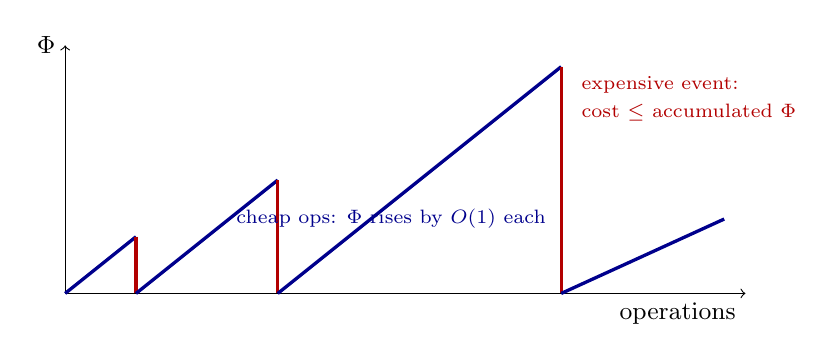
\begin{tikzpicture}[scale=0.9]
  \draw[->] (0,0) -- (9.6,0);
  \node[font=\small, below left] at (9.6,0) {operations};
  \draw[->] (0,0) -- (0,3.5);
  \node[font=\small, left] at (0,3.5) {$\Phi$};
  \draw[very thick, blue!55!black] (0,0) -- (1,0.8);
  \draw[very thick, red!70!black] (1,0.8) -- (1,0);
  \draw[very thick, blue!55!black] (1,0) -- (3,1.6);
  \draw[very thick, red!70!black] (3,1.6) -- (3,0);
  \draw[very thick, blue!55!black] (3,0) -- (7,3.2);
  \draw[very thick, red!70!black] (7,3.2) -- (7,0);
  \draw[very thick, blue!55!black] (7,0) -- (9.3,1.05);
  \node[font=\scriptsize, blue!55!black] at (4.6,1.05)
    {cheap ops: $\Phi$ rises by $O(1)$ each};
  \node[font=\scriptsize, red!70!black, anchor=west] at (7.15,2.95)
    {expensive event:};
  \node[font=\scriptsize, red!70!black, anchor=west] at (7.15,2.55)
    {cost $\le$ accumulated $\Phi$};
\end{tikzpicture}
\caption{The sawtooth: cheap operations deposit into $\Phi$; an expensive
event fires only when enough has accumulated, and its cost is paid entirely
by the drop in $\Phi$. Doubling the event cost doubles the inter-event gap.}
\label{fig:amo-sawtooth}
\end{figure}

The fourth rung packages the aggregate method for periodic structure --- and
it is the form most corpus papers actually use, because a batch schedule is
easier to name than a potential:

\begin{proposition}[Epoch decomposition]\label{prop:amo-epoch}
Partition every execution into consecutive \emph{epochs}, epoch $e$ having
$\mathrm{len}(e)$ operations and total cost $\mathrm{cost}(e)$. Then the
amortized cost per operation is $\sum_e \mathrm{cost}(e) / \sum_e
\mathrm{len}(e)$. In particular, if every epoch costs $O(C)$ and contains at
least $\ell$ operations, the amortized cost is $O(C/\ell)$; if an epoch's
fixed setup $S$ services $T$ operations, its contribution is $O(S/T)$. \eop
\end{proposition}

\begin{proof}
Sum epoch costs, sum epoch lengths, divide; the special cases substitute the uniform bounds.
\end{proof}

\sidenote{Epochs are the aggregate method in periodic clothing, and the
potential method is the accounting method with the balance read off the
state instead of the history; the three proofs are one proof --- sum a
nonnegative quantity --- and the choice is ergonomic: batch schedules state
epochs, accumulation triggers state $\Phi$.}
Sections~\ref{sec:amo-aero} and~\ref{sec:amo-order} below are epoch
arguments; Section~\ref{sec:amo-spline} is a pure potential argument.

\begin{remarkbox}[Notation]
Throughout, $c_i$ is the true cost of operation $i$, $\hat{a}_i$ its amortized
cost, and $\Phi$ a function from states to $\mathbb{R}_{\ge 0}$ with
$\Phi(D_0) = 0$ on the initial state. ``Amortized $O(f)$'' always means
total cost $O(mf)$ for every $m$ and every sequence of $m$ operations from
$D_0$ --- a deterministic statement about worst sequences, with nothing
averaged and nothing probabilistic (per-operation \emph{expected} cost is a
different, randomized contract).
\end{remarkbox}

The price of every rung is the same: the bound is a promise about
\emph{sequences}, not single operations. A deployment needing every request
answered within a deadline requires \emph{deamortized} variants that spread
each burst over neighboring operations \citep{amortized-potential-bg5}.

\subsection{How to choose the method}
\label{sec:amo-choose}

The selection is mechanical once two questions are answered. \emph{First, can
you sum a whole worst-case sequence?} If the total cost of $m$ operations has
a clean combinatorial bound, the aggregate method or its epoch packaging
(Proposition~\ref{prop:amo-epoch}) is the shortest honest proof.
\emph{Second, can you name who pays?} If the expensive event is triggered by
an accumulation you can point at --- rows since the last re-decomposition,
excess of a counter over its budget, rounding slack of a cached value ---
define $\Phi$ on exactly that quantity and verify the three properties of
Theorem~\ref{thm:amo-potential}. Use accounting when the payer is naturally
an operation (``this insert pays for its own future copy''), potential when
it is naturally a state (``every byte above the watermark''), and epochs
whenever the algorithm itself has a batch schedule.

\begin{reachbox}{When to Reach for Amortization}
Reach whenever a component must be certified with a \emph{per-operation}
time or space bound, the algorithm has an occasional expensive structural
event --- split, merge, rebuild, compaction, re-decomposition, full scan ---
and that event only fires after many cheap operations accumulate a trigger:
\begin{enumerate}
\item Identify the expensive rare operation: name the burst, its cost $C$,
  and the measurable quantity that must accumulate before it can fire again.
\item Define the potential on the state: $\Phi$ is that accumulated quantity
  (or the epoch schedule that bounds it), with $\Phi(D_0) = 0$.
\item Charge deposits and withdrawals: every cheap operation raises $\Phi$ by
  at most $O(1)$; every burst drops $\Phi$ by at least its cost $C$ --- so
  the inter-burst gap is $\Omega(C)$ and the amortized cost stays $O(1)$ per
  deposit.
\item Verify $\Phi \ge 0$ initially and throughout: this is what makes the
  telescoping safe for every prefix, and it is the only place amortized
  proofs fail --- one reachable state with $\Phi < 0$ voids the bound.
\end{enumerate}
Caveats before shipping the bound: amortized $\ne$ worst case (budget for
deamortization if tail latency matters), and insertion-only accumulation can
shatter under deletions --- check the fully dynamic lower bounds first.
\end{reachbox}

\section{Enumerating regular pattern matches with amortized constant delay}
\label{sec:amo-enum}

The exemplar is a PODS'26 paper on pattern matching \citep{sigmod26-177}\pods.
Extracting all matches of a \emph{pattern with variables} --- fixed
constants separated by variables standing for arbitrary substrings --- is
the engine behind regex-capture queries, log extraction, and transformation
languages; when the fixed parts are plain strings the pattern is called
\emph{regular}. A match assigns each variable a substring so that the
concatenation equals the text $T$, recorded by the $k$-tuple of positions
where the constants sit. Enumeration algorithms are judged on preprocessing
time, \emph{delay} between outputs, and space; the paper pushes all three to
optimal for this class, including an \emph{amortized} constant-delay
variant and an indexed version answering each later pattern in time
near-linear in the pattern alone --- reported as the first optimal
combined-complexity algorithms for a non-trivial subcase of enumerating
regular-expression matches with capture variables.

\paragraph{Problem.}
Let $T[1..n]$ be a text and $\alpha = w_0 \diamond x_1 w_1 \diamond \dots
\diamond x_k w_{k+1}$ a regular pattern with $\sum_{i=1}^{k} |w_i| \le n$. A
\emph{valid embedding} is a $k$-tuple $(j_1, \dots, j_k)$ such that $w_i$
occurs at position $j_i$ for each $i$, the occurrences are consecutive and
non-overlapping, $w_0$ is a prefix of $T$, and $w_{k+1}$ is the suffix
starting after $j_k + |w_k| - 1$. The task is to enumerate the set $S$ of all
valid embeddings. The difficulty is the output: $|S|$ can reach $n^k$, so
materializing occurrence lists up front risks blowing past $O(n)$, while the
delay must stay constant however the outputs are distributed.

\paragraph{Guarantee.}

\begin{theorem}[Optimal enumeration, Theorems~1.1 and~1.2 of the paper,
notation cleaned]\label{thm:amo-enum}
(i) The set $S$ of all valid embeddings of $\alpha$ in $T$ can be enumerated
with constant delay after preprocessing in $O(n + |S|)$ time, using
$O(n + \min\{|S|, n^k\})$ space. (ii) Alternatively, $S$ can be enumerated
with amortized constant delay after preprocessing in $O(n)$ time and the same
space: for every $s \le |S|$, the first $s$ embeddings are reported in
$O(n + s)$ total time. \eop
\end{theorem}

\sidenote{A third theorem of the paper upgrades to \emph{worst-case}
constant delay with $O(n)$ preprocessing at the price of
$O(n \min\{|S|, n^k\})$ space --- the deamortization trade of
Section~\ref{sec:amo-tool}.}
\paragraph{How amortization is applied.}
The variant (ii) is an aggregate-method argument over the enumeration phase,
and its engine is a counting bound on where embeddings can live. The paper
greedily computes a \emph{left-canonical} embedding $(\ell_1, \dots, \ell_k)$
(each $\ell_i$ the leftmost feasible occurrence of $w_i$) and a symmetric
\emph{right-canonical} embedding $(r_1, \dots, r_k)$; every valid embedding
$(j_i)$ satisfies $\ell_i \le j_i \le r_i$. Write $O_i = \{p \in [\ell_i :
r_i] \mid w_i \text{ occurs at } p\}$; the workhorse is the following bound.

\begin{lemma}[Embedding counting bound, Lemma~3.4 of the paper, notation
cleaned]\label{lem:amo-embed-count}
With $O_i$ and $S$ as above,
$\textstyle\sum_{i=1}^{k} (|O_i| - 1) \le \min\{kn,\ |S|\}$. \eop
\end{lemma}

\begin{proof}[Proof sketch]
$|O_i| \le n$ gives the $kn$ side. For the $|S|$ side, each $j_i \in O_i
\setminus\{\ell_i\}$ substituted into the canonical hybrid yields a valid
embedding, one distinct embedding per pair $(i, j_i)$. (Full proof in
Section~\ref{sec:amo-appendix}.)
\end{proof}

The algorithm runs in two phases. In preprocessing, the intervals
$[\ell_i : r_i + |w_i|)$ are partitioned into \emph{epochs}
(Definition~3.7 of the paper): maximal runs of intervals overlapping
transitively, whose left and right parts are separately pairwise disjoint,
so the total epoch length is $O(n)$. Each epoch is preprocessed
\emph{locally}, in time linear in its length: per-epoch suffix-array and
suffix-tree ranges for the $w_i$ (Lemma~2.2 of the paper), plus a
range-maximum structure enumerating with worst-case constant delay all
suffix-array entries above a threshold (Lemma~2.4). The amortization lives
in the enumeration phase: rather than materializing all lists $O_i$ during
preprocessing (their total length can exceed $n$), the algorithm outputs
the \emph{simple} embeddings --- those differing from the canonical
skeletons in exactly one coordinate --- \emph{while} building the lists,
one output per list element. Lemma~\ref{lem:amo-embed-count} bounds the
simple embeddings by $\min\{kn, |S|\}$, so every unit of
list-materialization work is paid for by an emitted embedding, up to
$O(n + k)$ overhang: the first $s$ embeddings cost $O(n + s)$ total. Once
the lists exist, a radix sort plus constant-delay enumeration (Lemma~3.6)
finishes.

\paragraph{What it buys.}
Preprocessing linear in $n$ \emph{independent of the output size},
amortized constant delay, and space $O(n + \min\{|S|, n^k\})$ --- plus the
indexed variant (each pattern answered in $O(|\alpha| + k \log n)$ plus
constant delay), the shape a database system needs for repeated extraction
queries.

\section[Matrix sketches for streams]{Matrix sketches for streams: batching the re-decomposition}
\label{sec:amo-aero}

The exemplar is a SIGMOD'26 paper on streaming matrix sketches
\citep{sigmod26-015}. A matrix sketch tracks the covariance structure of a
stream of $d$-dimensional row vectors --- the substrate for PCA-style
monitoring, regression, and anomaly detection --- and the standard tool,
Frequent Directions, periodically compresses its summary by an SVD. The
pain: a faithful SVD costs time quadratic in the error parameter, too
expensive to redo on every arrival. The paper proposes AeroSketch, keeping
the same space and error contracts while driving the amortized per-update
time down to what it calls near-optimal, across persistent streams,
sliding windows (only the last $N$ updates matter), and distributed sites
coordinating through a hub. The guarantees hold with tunable high
probability, inherited from iteration error bounds for randomized power
iterations --- and the time bounds are amortized, exactly the
batch-schedule amortization of Proposition~\ref{prop:amo-epoch}.

\paragraph{Problem.}
A stream presents row vectors $a_1, a_2, \dots \in \mathbb{R}^d$ one at a
time; stacking the arrivals so far gives $A$. The sketch $B$ must maintain
the covariance-error guarantee $\| A^{\top} A - B^{\top} B \|_2 \le
\varepsilon \|A\|_F^{2}$, preserving the top of the spectrum. In the
\emph{persistent} setting $A$ is the entire history; in the
\emph{sliding-window} setting only $(T-N, T]$ counts; in the
\emph{distributed} setting $m$ sites observe substreams while a
coordinator keeps the global sketch with bounded communication. The cost
model charges amortized time per update, space, and communication, with
success probability $1 - \delta$ for tunable $\delta$.

\paragraph{Guarantee.}

\begin{theorem}[Tracking matrix sketches, main theorems of the paper,
notation cleaned, $\varepsilon$-dependence restored]
\label{thm:amo-aero}
AeroSketch solves the persistent matrix-sketch tracking problem with space
$O\bigl(\tfrac{d}{\varepsilon} \log \|A\|_F^{2}\bigr)$ and amortized time
$O\bigl(\tfrac{d}{\varepsilon} \log d\bigr)$ per update, with success
probability at least $\tfrac{99}{100}\bigl(1 - \tfrac{2}{\sqrt{e}} \cdot
\tfrac{1}{\sqrt{d \log_2 d}}\bigr)$; with probability amplification it
achieves amortized time $O\bigl(\tfrac{d}{\varepsilon} \log d \log^{2}
\tfrac{1}{\delta}\bigr)$ per update while guaranteeing success probability
at least $1 - \delta$, for tunable $\delta \in (0, 1/100)$; the
sliding-window variant pays an extra $\log R$ in space and amortized
time. \eop
\end{theorem}

\paragraph{How amortization is applied.}
The expensive rare operation is the re-decomposition: when the sketch matrix
$C$ has absorbed $2/\varepsilon$ rows, an eigen-decomposition compresses it
back to $1/\varepsilon$ rows. The paper batches it exactly as in
Proposition~\ref{prop:amo-epoch}:

\begin{lemma}[Batched re-decomposition, Proposition of the paper and its
proof, notation cleaned, $\varepsilon$ restored]\label{lem:amo-aero-batch}
Between two consecutive re-decompositions at least $1/\varepsilon$ updates
elapse (the row count grows by one per update, from $1/\varepsilon$ back up
to $2/\varepsilon$). Each re-decomposition costs $O(d/\varepsilon^{2})$, so
its amortized contribution is $O(d/\varepsilon)$ per update; the per-update
power iteration monitoring the top singular value uses $k = \log_2 d + 1$
steps and costs $O(d \log d)$. Together, the amortized per-update time is
$O\bigl(\tfrac{d}{\varepsilon} \log d\bigr)$. \eop
\end{lemma}

\begin{proof}[Proof sketch]
Rows enter one per update; the decomposition fires exactly when the row count
reaches $2/\varepsilon$ and resets it to $1/\varepsilon$, so every epoch has
length at least $1/\varepsilon$ and one burst of $O(d/\varepsilon^2)$;
divide (full proof in Section~\ref{sec:amo-appendix}).
\end{proof}

The same accounting controls space: a re-decomposition \emph{dumps}
directions $Z_i$ (rank $k_i$) into a snapshot queue, and a dump fires only
after the sketch's residual Frobenius mass above a threshold $\theta$ has
accumulated by $k_i\theta/2$, so the dumped ranks sum to $O(\|A\|_F^2/
\theta)$ --- an implicit potential on the residual mass bounding the
queue. The \emph{whp} part: the re-decomposition only needs its top
singular values approximately; power iteration with $\log_2 d + 1$ steps
fails to halve the top squared singular value with probability at most
$\tfrac{2}{\sqrt{e}} \cdot \tfrac{1}{\sqrt{d \log_2 d}}$ (a corollary in
the paper), which is the success probability of
Theorem~\ref{thm:amo-aero}; amplification repeats the iteration and costs
the $\log^{2}(1/\delta)$ factor. The \emph{composition} part:

\begin{lemma}[Decomposability, Lemma of the paper, notation cleaned]
\label{lem:amo-aero-decomp}
Decompose $A = [A_1, A_2, \dots, A_m]$ into submatrices. If each $B_i$
sketches $A_i$ with covariance error $\|A_i^{\top} A_i - B_i^{\top}
B_i\|_2 \le \varepsilon_i \|A_i\|_F^{2}$, then $B = [B_1, B_2, \dots, B_m]$
sketches $A$ with $\| A^{\top} A - B^{\top} B \|_2 \le
\textstyle\sum_{i=1}^{m} \varepsilon_i \|A_i\|_F^{2}$. \eop
\end{lemma}

\begin{proof}
$A^{\top} A - B^{\top} B = \sum_i (A_i^{\top} A_i - B_i^{\top} B_i)$;
apply the triangle inequality to the spectral norm and substitute each
block's guarantee.
\end{proof}

Sliding windows and distributed sites both become substreams (snapshots are
blocks whose per-block errors add, decomposability summing them), with
communication bounded by the same epoch counting on rounds of a doubling
threshold. The per-update error telescopes over the window: the
accumulated spectral error is the sum of discarded singular values, which
the dump-threshold accounting keeps within $O(\varepsilon)\|A\|_F^2$.

\paragraph{What it buys.}
Amortized $O\bigl(\tfrac{d}{\varepsilon} \log d\bigr)$ per update instead
of an $O(d/\varepsilon^2)$ burst every $\tfrac{1}{\varepsilon}$ updates ---
one proof skeleton covering persistent, sliding-window, and distributed
deployments, with tunable success probability.

\section{Order routing in exchange graphs: epochs over path selections}
\label{sec:amo-order}

The exemplar is a SIGMOD'26 paper on order routing in decentralized finance
\citep{sigmod26-180}. A decentralized exchange is a graph: token pairs are
joined by pools quoting a price (a \emph{weight}) with limited liquidity (a
\emph{capacity}). Routing a market order means repeatedly picking the
cheapest path in this \emph{exchange graph}, executing against it until a
bottleneck capacity is exhausted, re-pricing, and picking again --- and
since every fill moves prices and depletes capacities, the ranking of paths
goes stale after each selection, while re-scanning all candidates after
every fill is quadratic in the path count. The paper builds ORDER, a
path-indexing structure whose maintenance is \emph{lazy} --- cached weights
and capacities refresh only when a correctness invariant demands it ---
certified by an amortized complexity theorem over \emph{epochs} of
selections: contradiction proofs on the global weight ordering prove the
laziness safe, an epoch decomposition proves it cheap.

\paragraph{Problem.}
For each token pair $(u,v)$ an \emph{ordered edge group} $E_g(u,v)$ holds
the parallel edges (feasible swaps) sorted by nondecreasing weight
$w_\ell$, each with capacity $c_\ell$; the \emph{front} of a group is its
minimum-weight edge with remaining capacity. A path $\pi$ carries the
ordering key $W(\pi) = \sum_{g \in \pi} w_g$ (sum of front weights) and
the bottleneck capacity $C(\pi) = \min_{g \in \pi} c_g$. The iterative
selection loop repeatedly extracts the minimum-key path, executes an
amount, consumes capacities along the path (possibly advancing fronts),
and re-ranks. ORDER maintains an \emph{active bucket} --- a heap over the
top-$K$ paths by key --- plus \emph{reserve buckets} holding the remaining
candidates in coarser weight ranges, replenished by periodic rebuilds.

\paragraph{Guarantee.}

\begin{theorem}[Amortized complexity, Theorem~3.9 of the paper, notation
cleaned]\label{thm:amo-order-amort}
Consider the iterative path-selection algorithm over $|P|$ indexed paths
with active-bucket size $K$. One rebuild epoch with $T$ selection
iterations costs $O(|P|) + O(K \log K) + O(T \log K)$, so the amortized
time per selection iteration is $O\bigl(\tfrac{|P|}{T}\bigr) +
O\bigl(\tfrac{K \log K}{T}\bigr) + O(\log K)$. \eop
\end{theorem}

\paragraph{How amortization is applied.}
The proof (transcribed in Section~\ref{sec:amo-appendix}) is a textbook
epoch decomposition in the sense of Proposition~\ref{prop:amo-epoch}: an
epoch is (1)~one scan of all $|P|$ paths recomputing keys and admitting
the top $K$ into the active bucket via a KLL-style quantile sketch, (2)~the
build of that bucket, a heap over at most $K$ paths, and (3)~the $T$
selections, each an extract-min plus a bounded number of localized heap
updates at $O(\log K)$ apiece. The amortization invariant is that the $K$
admitted paths are all consumed \emph{within that same epoch} --- extracted
or evicted --- so the fixed costs (1)--(2) are spread over exactly the $T$
selections they service. What keeps the lazy structure \emph{correct}
while cheap is a pair of contradiction arguments on the ordering of keys:

\begin{lemma}[No-cross-bucket domination, Lemma~4.2 of the paper, notation
cleaned]\label{lem:amo-order-nodom}
Given the prioritized buckets, for any two bucket indices $i < i'$, no path
in $B_{i'}$ has a strictly smaller ordering key than a path in $B_i$:
$\pi_p \in B_i,\ \pi_q \in B_{i'},\ i < i' \Rightarrow W(\pi_p) \le
W(\pi_q)$. \eop
\end{lemma}

\begin{proof}[Proof sketch]
Buckets partition a global sort of paths by $W(\cdot)$ into index-ordered,
non-overlapping ranges; a strict reversal would place $\pi_q$ before $\pi_p$
in that sort, forcing it into a bucket of index at most $i$, contradicting
$\pi_q \in B_{i'}$ with $i' > i$.
\end{proof}

Domination means selection never looks past the active bucket until it is
exhausted; a companion rebuild-truncation lemma shows a rebuild can stop
early while some reserve path is unaffected by recent updates, and an
on-demand bottleneck lemma (Lemma~3.4 of the paper) shows the bottleneck
read off the \emph{current fronts} at selection time already equals the
true one --- so capacities too are maintained lazily, on demand.

\paragraph{What it buys.}
Each fill pays $O(\log K)$-ish maintenance instead of a full re-ranking,
while the routing output remains \emph{exactly} optimal --- laziness
certified safe by the ordering lemmas, not traded against approximation ---
and the epoch schedule says when to expect the next heavier rebuild bill.

\section{Quantile sketches: a potential over bucket counters}
\label{sec:amo-spline}

The exemplar is a SIGMOD'26 paper on quantile sketches \citep{sigmod26-363}.
Estimating quantiles over a stream --- medians, percentiles, heavy
thresholds --- is a core analytics primitive, and the classical
deterministic summaries (GK and its descendants, KLL) share a ceiling:
within a bucket, rank is interpolated under a uniformity assumption, and
that assumption is what their error bounds pay for. SplineSketch instead
interpolates the rank function inside each bucket by a \emph{spline}
(monotone cubic by construction), which tracks skewed data far better;
buckets carry counters, and the sketch stays at $k$ buckets through two
structural events --- a \emph{split} when a counter exceeds its budget and
a \emph{join} of adjacent buckets to reclaim space. The analysis questions
are exactly amortization questions --- how many splits can a stream force,
and how much rank error does each deposit? --- answered by an explicit
potential over the bucket counters, the purest $\Phi$-argument in this
chapter's corpus.

\paragraph{Problem.}
A stream of $n$ items arrives; the sketch keeps $k$ buckets over the value
range, bucket $i$ being an interval $(\sigma_{i-1}, \sigma_i]$ between
thresholds with a counter $b_i$ of absorbed items. Arrivals are buffered
and periodically merged into buckets; to keep at most $k$ buckets, a bucket
violating the \emph{bucket bound} $b_i \le C_b \cdot n/k$ must \emph{split},
and adjacent buckets are \emph{joined} to reclaim space --- a pair is
\emph{joinable} if the merged counter satisfies $b_i + b_{i+1} \le 0.75
\cdot C_b \cdot n/k$ and the threshold $\sigma_i$ is not \emph{protected}
(freshly created by a split). Queries are answered by the counters plus
spline interpolation inside each bucket. The task is to bound the number
of splits --- hence the protected thresholds, hence the ability to always
find a joinable pair --- and the resulting rank error.

\paragraph{Guarantee.}

\begin{theorem}[Rank error, from the paper's error analysis, notation
cleaned]\label{thm:amo-spline-error}
After processing $n$ items (with a Misra--Gries sketch of size $O(k)$
filtering heavy hitters in parallel), for any threshold $\sigma_i$ of the
final sketch the rank error obeys
\[
\varepsilon^{n}(\sigma_i) \;\le\; O\bigl(\log \alpha \cdot n/k\bigr),
\]
where $\alpha$ is the paper's aspect-ratio parameter of the stream; the
lower error is symmetric, and in the mergeable setting the bound is
$O\bigl(\log (n/k) \cdot n/k\bigr)$. \eop
\end{theorem}

\paragraph{How amortization is applied.}
Nothing here is random --- this is deterministic bookkeeping. The paper
defines the potential of a sketch state $S$ at time $t''$ with $k(S)$ buckets
as the total \emph{excess of the counters over the join budget}:
\[
\Phi(S) \;=\; \textstyle\sum_{i=1}^{k(S)} \max\Bigl\{\,0,\;
b_i - 0.75 \cdot C_b \cdot t''/k \,\Bigr\},
\]
and verifies exactly the reachbox recipe: $\Phi(S) \in [0, t'']$
(nonnegativity); each of the $t - t'$ arrivals in an interval $(t', t]$
increments one counter by one, raising $\Phi$ by at most $1$ (deposits,
total increase $\le t - t'$); joins never raise $\Phi$ (joinability keeps
the merged counter at or below the join budget, where the max-terms
vanish); and every forced split \emph{decreases} $\Phi$ by at least
$\beta \cdot C_b \cdot t / (2.5 k)$ for a placement constant $\beta$
(withdrawals). The workhorse is then pure division:

\begin{lemma}[Split budget, from the paper's analysis, notation cleaned]
\label{lem:amo-spline-split}
The number of splits during $(t', t]$ is at most
$\frac{t - t'}{\beta C_b t / (2.5 k)} = \frac{2.5\,k}{\beta C_b} \le
\frac{k}{18}$, with $C_b$ chosen as a function of $\beta$. \eop
\end{lemma}

\begin{proof}[Proof sketch]
Divide the total possible deposit $t - t'$ by the minimum withdrawal per
split; the withdrawal case analysis is in Section~\ref{sec:amo-appendix}.
\end{proof}

The split budget powers two conclusions. First, protected thresholds are
bounded (each split creates $O(1)$), so a counting argument shows the
sketch \emph{always} contains a joinable pair --- too many unjoinable
adjacent pairs would need more protected thresholds than splits can create
or more counter mass than $t$ items supply. Second, the rank error is
\emph{charged along the split history}: a threshold's error grows only at
splits, and each ancestor in the merge tree contributes a geometrically
shrinking share --- the same arithmetic in log scale, giving the
$O(\log \alpha \cdot n/k)$ bound. The spline itself contributes a
feasibility lemma proved by a coefficient argument:

\begin{lemma}[Spline midpoint bound, Lemma of the paper, notation cleaned]
\label{lem:amo-spline-midpoint}
Let $P(x)$ be a cubic polynomial with $P(0) = 0$, $P(1) = 1$, non-decreasing
on $[0,1]$. Then $P(\tfrac12) \in [\beta,\, 1 - \beta]$ with
$\beta = \tfrac12 - \tfrac{\sqrt{3}}{4} \approx 0.067$. \eop
\end{lemma}

\begin{proof}[Proof sketch]
Write $P(\lambda) = a\lambda^3 + b\lambda^2 + c\lambda$ with $a + b + c =
1$; monotonicity forces $3a\lambda^2 + 2b\lambda + c \ge 0$ on $[0,1]$, and
evaluating that constraint at one well-chosen test point bounds
$-(\tfrac{3a}{8} + \tfrac{b}{4})$, which is exactly $\tfrac12 -
P(\tfrac12)$. (Full proof, with the test point, in
Section~\ref{sec:amo-appendix}.)
\end{proof}

The lemma guarantees the interpolation inside any bucket is never
arbitrarily skewed at its midpoint --- the coefficient feasibility that
makes the spline's error arithmetic work with clean constants.

\paragraph{What it buys.}
$O(\log k)$ per operation via two heaps and a queue, deterministic and
mergeable with the stated error guarantees, and --- the experimental
headline --- noticeably more accurate quantiles than KLL and GK-style
baselines at equal space, because the potential certifies a thrifty split
schedule.

\section{Advanced usage and further reading}
\label{sec:amo-advanced}

The two usages sketched here compose the tool with other theory: an
amortized bound purchased at the price of approximation, certified
unavoidable by a lower-bound reduction; and an amortized update bound
riding a DP space optimization.

\paragraph{Approximate query processing under updates
\citep{sigmod26-274}.}
Maintaining the answer to a conjunctive query over a semiring under updates
is blocked, outside the tiny q-hierarchical class, by dynamic lower bounds:
any non-q-hierarchical Boolean CQ needs amortized $\Omega(\sqrt{N})$ update
time under fully dynamic sequences. The paper's escape splits the
free-connex join tree into an \emph{exact connex part} (helper views kept
exact, so enumeration stays constant-delay) and an \emph{approximated
part}, whose cached annotations are rounded to a factor $b$ and refreshed
lazily when the true value outgrows the cache. The potential is the total
rounding slack: an insertion deposits $O(1)$, a recomputation cascade fires
only when some tuple's slack is exhausted, and each tuple can fire at most
$\log_b M$ times, $M$ the largest annotation ever cached. The guarantee
(Theorem~4.7 of the paper): for any $b > 1$ and free-connex query, all
auxiliary views update in amortized $O(\log_b M)$ time under
insertion-only sequences (for the join size of a 3-way join, $O(\log_b
N)$). The hypothesis is necessary: any multiplicative approximation on the
semiring $(\mathbb{R}_{\ge 0}, +, \times)$ yields exact answers on the
Boolean semiring, so the $\Omega(\sqrt{N})$ fully-dynamic lower bound
transfers.

\paragraph{RadixGraph: amortized compaction over log segments
\citep{sigmod26-203}.}
RadixGraph is a dynamic graph storage structure: adjacency is compressed
into radix-tree layers over bit prefixes of vertex ids, and updates append
to log segments periodically \emph{compacted} back into the layers. The
layer structure is chosen by an occupancy model whose space objective is
minimized by a DP over layer splits, computable in $O(nlx^{2})$ time and
$O(lx)$ space. On top sits the amortized bound (Theorem and proof sketch
of the paper): edge insertion, update, and deletion cost amortized $O(1)$
--- appending to a non-full log segment costs $O(1)$, and when a segment
fills, the compaction costs $O(d)$ but is charged to the $\Omega(d)$
appends that must accumulate before it can fire, epoch counting in its
barest form.

\subsection{Further reading}

\begin{itemize}
\item The amortized-analysis chapters of Cormen et al.\
\citep{amortized-potential-bg3} --- aggregate, accounting, and potential
methods with the dynamic-table example.
\item Tarjan's survey \citep{amortized-potential-bg1}, with the union--find
and splay-tree classics \citep{amortized-potential-bg2}.
\item Overmars \citep{amortized-potential-bg5} --- periodic rebuilding as
the degenerate epoch schedule, and the deamortization caveats.
\item Greenwald and Khanna \citep{amortized-potential-bg4} --- quantile
summaries where potential-bounded compaction first appeared in the DB
literature; the ancestor of Section~\ref{sec:amo-spline}'s analysis.
\end{itemize}

\begin{recap}
\item \textbf{What the tool is.} Amortized analysis certifies per-operation
  time/space bounds over \emph{sequences}: bursts are rare because they
  require accumulation, and the certificate is a bank balance (accounting),
  a state function $\Phi \ge 0$ (potential), or a batch schedule (epochs).
\item \textbf{Which rung when.} Clean global sum of a worst-case sequence:
  aggregate. Explicit batch schedule (re-decompose every $\ell$ arrivals,
  rebuild after $T$ selections): epoch decomposition
  (Proposition~\ref{prop:amo-epoch}). Measurable state trigger (counter
  excess, rounding slack, residual mass): potential
  (Theorem~\ref{thm:amo-potential}). Payer naturally an operation:
  accounting (Theorem~\ref{thm:amo-accounting}).
\item \textbf{Why it works.} Telescoping: $\sum_i c_i = \sum_i \hat{a}_i -
  \Phi(D_m) \le \sum_i \hat{a}_i$ whenever $\Phi \ge 0$ and $\Phi(D_0) = 0$;
  the failure modes are a reachable state with $\Phi < 0$, or a burst that
  fires without its accumulation.
\item \textbf{What the corpus showed.} Pattern enumeration
  (Section~\ref{sec:amo-enum}): a counting bound pays for list
  materialization with outputs --- amortized $O(1)$ delay. Matrix sketches
  (Section~\ref{sec:amo-aero}): SVD bursts batched over $1/\varepsilon$
  arrivals, composed across windows and sites. Order routing
  (Section~\ref{sec:amo-order}): rebuild epochs over $T$ selections,
  contradiction proofs certifying lazy maintenance. Quantile sketches
  (Section~\ref{sec:amo-spline}): a potential over bucket counters bounds
  splits by $k/18$; rank error is charged along the split history.
\item \textbf{Advanced usage.} Amortization purchased with approximation
  ($O(\log_b M)$ updates at factor-$b$ rounding, lower bound imported by a
  Boolean-semiring reduction), and amortized $O(1)$ graph updates riding a
  DP-optimal layout (Section~\ref{sec:amo-advanced}). Deferred proofs are
  collected in the Appendix (Section~\ref{sec:amo-appendix}).
\end{recap}

\section{Appendix}
\label{sec:amo-appendix}

Proofs omitted from the main text are collected here.

\subsubsection*{Proof of Lemma~\ref{lem:amo-embed-count} (embedding counting)}
{\itshape Statement (recalled).} For the valid occurrence sets $O_i \subseteq
[\ell_i : r_i]$ of the constant strings $w_i$ and the set $S$ of all valid
embeddings, $\sum_{i=1}^{k} (|O_i| - 1) \le \min\{kn, |S|\}$.\eop

\begin{proof}
The bound $\sum_i (|O_i| - 1) \le kn$ is immediate from $|O_i| \le n$. For
the second bound, the paper's canonical-embedding lemma gives that for
$j_i \in O_i \setminus\{\ell_i\}$ the hybrid tuple $(\ell_1, \dots,
\ell_{i-1},\, j_i,\, r_{i+1}, \dots, r_k)$ is a valid embedding: anchoring
the prefix at the leftmost and the suffix at the rightmost feasible
occurrences leaves every intermediate valid occurrence of $w_i$ feasible.
So each $i$ yields $|O_i| - 1$ valid embeddings, pairwise distinct --- two
for the same $i$ differ in coordinate $i$, and two for $i_1 < i_2$ differ in
coordinate $i_1$. All lie in $S$, so $\sum_i (|O_i| - 1) \le |S|$.
\end{proof}

\subsubsection*{Proof of Lemma~\ref{lem:amo-aero-batch} (batched
re-decomposition)}
{\itshape Statement (recalled).} Re-decompositions fire at most once per
$1/\varepsilon$ updates, each costs $O(d/\varepsilon^{2})$, and the
per-update power iteration costs $O(d \log d)$; the amortized per-update
time is $O\bigl(\tfrac{d}{\varepsilon} \log d\bigr)$.\eop

\begin{proof}
The sketch matrix $C$ gains one row per update; the re-decomposition
triggers when the row count reaches $2/\varepsilon$ and resets it to
$1/\varepsilon$, so consecutive triggers are at least $\tfrac{1}{\varepsilon}$
updates apart --- epochs of Proposition~\ref{prop:amo-epoch} with
$\ell = 1/\varepsilon$. The trigger costs the eigen-decomposition of a
$d \times \tfrac{2}{\varepsilon}$ matrix, $O(d/\varepsilon^{2})$ in the
paper's accounting, an amortized $O(d/\varepsilon)$ per update.
Independently, every update runs a power iteration with $k = \log_2 d + 1$
matrix--vector products, $O(d\log d)$, against the dump threshold. Since
$d \log d \le \tfrac{d}{\varepsilon} \log d$ for $\varepsilon \le 1$, the
contributions sum to $O\bigl(\tfrac{d}{\varepsilon} \log d\bigr)$
amortized per update.
\end{proof}

\subsubsection*{Proof of Theorem~\ref{thm:amo-order-amort} (epoch accounting)}
{\itshape Statement (recalled).} One rebuild epoch with $T$ selections costs
$O(|P|) + O(K \log K) + O(T \log K)$, so the amortized time per selection is
$O\bigl(\tfrac{|P|}{T}\bigr) + O\bigl(\tfrac{K \log K}{T}\bigr) +
O(\log K)$.\eop

\begin{proof}
Decompose the epoch as in the paper's proof. (1) \emph{Scan and admission},
$O(|P|)$: all $|P|$ paths are visited once to recompute weights and assign
reserve-bucket ranges; the top $K$ are selected through a KLL-style
quantile sketch, which returns the admission threshold and emits the top
$K$ items. (2) \emph{Active-bucket build}, $O(K \log K)$: a binary heap
over at most $K$ paths. (3) \emph{Per-selection maintenance},
$O(T \log K)$: each selection is one extract-min plus $O(1)$ localized
heap updates at $O(\log K)$ each. The amortization invariant --- every
path admitted in (1) is consumed within the same epoch --- ensures the
fixed costs (1)--(2) are covered by exactly the $T$ selections they
service; summing and dividing by $T$ (Proposition~\ref{prop:amo-epoch})
yields the per-iteration bound.
\end{proof}

\subsubsection*{Proof of Lemma~\ref{lem:amo-spline-split} (split budget)}
{\itshape Statement (recalled).} With
$\Phi(S) = \sum_{i=1}^{k(S)} \max\{0, b_i - 0.75 \cdot C_b \cdot t''/k\}$,
the number of splits during $(t', t]$ is at most
$\tfrac{2.5 k}{\beta C_b} \le \tfrac{k}{18}$.\eop

\begin{proof}
Write $\tau_J = 0.75 \cdot C_b \cdot t''/k$ for the join budget at time
$t''$. \emph{Deposits:} each of the $t - t'$ arrivals increments one
counter by one, so $\Phi$ rises by at most $1$ per arrival (total increase
$\le t - t'$), and $\Phi \ge 0$ throughout since every summand is
nonnegative. \emph{Joins:} joinability gives $b_i + b_{i+1} \le \tau_J$,
so the pre-join summands and the post-join one vanish; joins never
increase $\Phi$. \emph{Withdrawals:} a split at time $t'' \in (t', t]$
fires on a bucket with $b_i > C_b t''/k$, whose summand contributes
$b_i - \tau_J > 0.25\,C_b t''/k$; the split places the new threshold so
each child receives at least a $\beta$-fraction of the parent's counter
($2.5 = 1/\beta$). If both children have counters $\ge \tau_J$, the
decrease is exactly $\tau_J \ge 0.75\,C_b t''/k$; otherwise the smaller
child's summand vanishes and the decrease is at least that counter,
$\ge \beta b_i > \beta C_b t''/k \ge \beta C_b t/(2.5k)$ (using
$t'' \le t$) --- the paper's uniform withdrawal, met in both cases.
\emph{Division:} total decrease cannot exceed total increase, so splits
number at most $\frac{t - t'}{\beta C_b t/(2.5k)} = \frac{2.5k}{\beta C_b}
\le k/18$, by the paper's calibration of $C_b$ from $\beta$.
\end{proof}

\subsubsection*{Proof of Lemma~\ref{lem:amo-spline-midpoint} (spline
midpoint)}
{\itshape Statement (recalled).} If $P$ is cubic with $P(0) = 0$, $P(1) = 1$,
non-decreasing on $[0,1]$, then $P(\tfrac12) \in
[\tfrac12 - \tfrac{\sqrt3}{4},\, \tfrac12 + \tfrac{\sqrt3}{4}]$.\eop

\begin{proof}
By symmetry ($Q(x) = 1 - P(1-x)$ is again cubic, non-decreasing, with
$Q(\tfrac12) = 1 - P(\tfrac12)$) it suffices to prove
$P(\tfrac12) \le \tfrac12 + \tfrac{\sqrt{3}}{4}$. Write
$P(\lambda) = a\lambda^{3} + b\lambda^{2} + c\lambda$: $P(1) = 1$ gives
$a + b + c = 1$, and monotonicity gives $P'(\lambda) = 3a\lambda^{2} +
2b\lambda + c \ge 0$ on $[0,1]$. Since $P(\tfrac12) = \tfrac12 -
(\tfrac{3a}{8} + \tfrac{b}{4})$, it remains to bound
$-(\tfrac{3a}{8} + \tfrac{b}{4})$. Substituting $c = 1 - a - b$ into the
derivative constraint and evaluating at the test point $\lambda^{*} =
\tfrac{3+\sqrt{3}}{6} \in [0,1]$, where $3\lambda^{*2} - 1 =
\tfrac{\sqrt{3}}{2}$ and $2\lambda^{*} - 1 = \tfrac{\sqrt{3}}{3}$, yields
\[
0 \;\le\; (3\lambda^{*2} - 1)\,a + (2\lambda^{*} - 1)\,b + 1
\;=\; \sqrt{3}\Bigl(\tfrac{a}{2} + \tfrac{b}{3}\Bigr) + 1,
\]
so $\tfrac{a}{2} + \tfrac{b}{3} \ge -\tfrac{1}{\sqrt{3}}$; multiplying by
$-\tfrac34$ gives $-(\tfrac{3a}{8} + \tfrac{b}{4}) \le
\tfrac{3}{4\sqrt{3}} = \tfrac{\sqrt{3}}{4}$, hence the claim by symmetry.
\end{proof}

\bibliographystyle{plainnat}
\bibliography{chapters/amortized-potential-all}

\chapter{Coresets and Randomized Numerical Linear Algebra}
\setcounter{section}{-1}   % sections start at 12.0 (see main.tex comment)
\label{ch:coresets}

% ROLLOUT STUB (round 6) -- being written to the pilot spec (CHAPTER-RULES.md).
% Exemplars per plan.json (merged coresets-geometry + randomized-nla): 289,
% 053, 303, 349, 052, 127.
This chapter is being revised; see Chapter~\ref{ch:intro} for the survey
context in the meantime.

\chapter{Information-Theoretic Arguments}
\setcounter{section}{-1}   % sections start at 11.0 (see main.tex comment)
\label{ch:inf}

\begin{objectives}
\item Recognize information-theoretic claims: content bounds (bits) or distinguishability bounds (divergence).
\item Prove the ladder: source coding $\to$ chain rule $\to$ KL/R\'enyi and Pinsker $\to$ incompressibility $\to$ Fano.
\item Match measure to task: entropy for space, KL for error, R\'enyi for composed stages, Fano for impossibility.
\item Dissect a paper's argument: random object, measure, chain-rule telescope, final bound.
\end{objectives}

Information theory counts information. Its two workhorses --- the \emph{entropy} of a
distribution (information content) and the \emph{divergence} between two distributions
(distinguishability) --- set limits no algorithm, protocol, or noise mechanism can
beat, in both directions. Downward: a quantity of $H$ bits can be written down in
about $H$ bits --- how sketches and compressible counters justify their footprint.
Upward: a task implicitly identifying one of $M$ objects forces $\log M$ bits --- how
space lower bounds and impossibility results are proved. Divergences do the same for
pairs: differential privacy \emph{is} a divergence bound between outputs on
neighboring inputs; a synthesizer's accuracy is a divergence to the truth.

In the SIGMOD'26 corpus the tool is tagged in a small cohort (5 papers) with a clean
division of labor: error bounds in three of the five (frequency-estimation sketching,
private query processing, private data-synthesis benchmarking), space lower bounds and
privacy guarantees in two each, and a PODS'26 entry that turns Shannon inequalities
directly into a join algorithm. Two exemplars (DP-S4S, Sublime) recur from
Chapters~\ref{ch:conc} and~\ref{ch:est}, but their information-theoretic side is a
different object from the side treated there. Section~\ref{sec:inf-advanced} adds
entropy as a difficulty measure, and further reading.

\section{The tool: information theory}

The problem class is uniform. Somewhere in the system there is a random object --- a
stream prefix, a pair of neighboring databases, a hypothesis about the data --- and the
question is not how a computation behaves \emph{on average} (Chapter~\ref{ch:conc}) but
how much \emph{information} the object carries, or how \emph{distinguishable} two of
its instantiations are. An entropy of $H$ bits is both a guarantee (an encoding of
length $\approx H$ exists) and a barrier (nothing shorter suffices).

\begin{remarkbox}[Notation]
Logs are base~2 (\emph{bits}) except for divergences $D$, $D_\alpha$, in \emph{nats}
(the divergence/privacy convention). $H(X)$: entropy of $X$; lowercase $h(X)$: the
\emph{entropy function} of a joint distribution viewed as a set function on attribute
sets (the join-processing usage). $p \ll q$: $q(x) = 0 \Rightarrow p(x) = 0$.
\end{remarkbox}

\subsection{The basic ladder}
\label{sec:inf-ladder}

\begin{definition}[Shannon entropy]\label{def:inf-entropy}
For a discrete random variable $X$ with distribution $p$, the \emph{entropy} is
\[
H(X) \;=\; -\sum_{x} p(x)\,\log_2 p(x) \qquad (0\log 0 := 0),
\]
and the \emph{conditional entropy} of $X$ given $Y$ is
$H(X \mid Y) = \sum_y \Pr[Y = y]\,H(X \mid Y = y)$. Entropy measures the number of bits
needed, on average, to pin down the value of $X$.
\end{definition}

The first rung makes that sentence a theorem \citep{information-theory-bg1,
information-theory-bg2}: no lossless code beats the entropy, and one within a bit
exists (``code'' = prefix-free binary description).

\begin{theorem}[Source-coding bound]\label{thm:inf-source}
Let $\ell\colon \mathcal{X} \to \mathbb{N}$ be the length function of any prefix-free
binary code for $X$. Then
\[
\mathbb{E}[\ell(X)] \;\ge\; H(X), \eopm
\]
with equality iff $\ell(x) = -\log_2 p(x)$. Conversely, the Shannon code $\ell(x) =
\lceil -\log_2 p(x)\rceil$ is prefix-free with $\mathbb{E}[\ell(X)] < H(X) + 1$.
\end{theorem}

\begin{proof}
Codewords are disjoint leaves of a binary tree, so Kraft's inequality gives
$Z := \sum_x 2^{-\ell(x)} \le 1$; set $q(x) = 2^{-\ell(x)}/Z$. Writing $D_2$ for the
KL divergence of Definition~\ref{def:inf-kl} in bits,
\[
D_2(p\|q) \;=\; \sum_x p \log_2\frac{p}{q}
\;=\; -H(X) + \mathbb{E}[\ell] + \log_2 Z \;\ge\; 0
\]
by Gibbs (Lemma~\ref{lem:inf-gibbs}); $\log_2 Z \le 0$ gives $\mathbb{E}[\ell] \ge
H(X)$, equality iff $q = p$, $Z = 1$. Conversely $\ell(x) = \lceil -\log_2 p(x)\rceil$
satisfies $2^{-\ell(x)} \le p(x)$, so Kraft holds, and $\ell < -\log_2 p + 1$.
\end{proof}

The second rung lets entropy telescope over multi-part objects --- the step that turns
a pipeline into an equation.

\begin{proposition}[Chain rule and conditioning]\label{prop:inf-chainrule}
For any pair of random variables,
\[
H(X,Y) \;=\; H(X) + H(Y \mid X),
\qquad\text{hence}\qquad
H(Y \mid X) \;\le\; H(Y),
\]
with equality in the second inequality iff $X$ and $Y$ are independent. \eop
\end{proposition}

\begin{proof}
Write $\log_2 p(x,y) = \log_2 p(x) + \log_2 p(y \mid x)$ and take $-\mathbb{E}$;
$H(Y|X) \le H(Y)$ follows by Jensen ($\log$ concave) over the average in $x$.
\end{proof}

The join-processing application needs the set-function form $h(X) = H(X)$, $X \subseteq
V$, for a joint distribution over variables $V$.

\begin{corollary}[Entropy is submodular; polymatroids]\label{cor:inf-submodular}
For all $X, Y, Z \subseteq V$:
\[
h(XY) + h(XZ) \;\ge\; h(X) + h(XYZ), \qquad h(XY) \ge h(X) \ge h(\emptyset) = 0.
\]
That is, the entropy function of any joint distribution is a \emph{polymatroid}
(normalized, monotone, submodular); inequalities valid for all polymatroids are called
\emph{Shannon inequalities}. \eop
\end{corollary}

\begin{proof}
$h(XY) + h(XZ) - h(XYZ) - h(X) = I(Y;Z \mid X) = H(Y|X) - H(Y|XZ) \ge 0$ by
Proposition~\ref{prop:inf-chainrule} applied twice; monotonicity is $H(Y|X) \ge 0$.
\end{proof}

The third rung measures distinguishability of two distributions
\citep{information-theory-bg2, information-theory-bg3}.

\begin{definition}[KL divergence]\label{def:inf-kl}
For distributions $p, q$ with $p \ll q$, the \emph{Kullback--Leibler divergence} is
\[
D(p \,\|\, q) \;=\; \sum_x p(x)\,\ln\frac{p(x)}{q(x)} \qquad (\text{nats}),
\]
and $D(p\|q) = \infty$ if $p \not\ll q$.
\end{definition}

\begin{lemma}[Gibbs]\label{lem:inf-gibbs}
$D(p\|q) \ge 0$ with equality iff $p = q$. \eop
\end{lemma}

\begin{proof}
$-D(p\|q) = \sum_x p(x)\ln\frac{q(x)}{p(x)} \le \ln\sum_x q(x) \le 0$ by Jensen
applied to the concave $\ln$ (the sum runs over $\operatorname{supp} p$).
\end{proof}

Two structural facts convert divergences along pipelines; both are one application of
the log-sum inequality \citep{information-theory-bg2} and both recur in the exemplars.

\begin{proposition}[Mixture convexity, chain rule, data processing]\label{prop:inf-klmix}
\leavevmode
\begin{enumerate}
\item (Convexity in the mixture.) If $P_i, Q_i$ are distributions and $\beta_i \ge
0$, $\sum_i \beta_i = 1$, then $D(\sum_i \beta_i P_i \,\|\, \sum_i \beta_i Q_i)
\le \sum_i \beta_i\,D(P_i \| Q_i)$.
\item (Chain rule.) With the same mixing distribution on both sides, the joint divergence
is the average of the conditional divergences:
\[
D(p(x)P(z|x) \,\|\, p(x)Q(z|x)) \;=\; \sum_x p(x)\,
D(P(\cdot|x) \,\|\, Q(\cdot|x)).
\]
Consequently
(data processing for a partition) $D(p\|q) \ge d(p(E) \| q(E))$ for every event $E$,
with $d$ the two-point divergence. \eop
\end{enumerate}
\end{proposition}

\begin{proof}[Proof sketch]
Expand $\sum_{x,z} p(x)P(z|x)\ln\frac{P(z|x)}{Q(z|x)}$: the $p(x)$ terms cancel,
giving (ii); (i) is the log-sum inequality applied per outcome. For the last claim,
let $z$ be the cell indicator of $E$ and drop the second, nonnegative term of (ii).
\end{proof}

Divergence controls total variation --- the bridge from information to probability:

\begin{theorem}[Pinsker]\label{thm:inf-pinsker}
For all $p, q$,
\[
\operatorname{TV}(p,q) \;:=\; \tfrac12 \sum_x |p(x) - q(x)| \;\le\;
\sqrt{\tfrac12 D(p\|q)}. \eopm
\]
\end{theorem}

\begin{proof}[Proof sketch]
Data processing (Proposition~\ref{prop:inf-klmix}) reduces to two points at the event
$E$ achieving total variation, $a = \Pr_p(E) > b = \Pr_q(E)$. The two-point divergence
has $\partial_b d(a\|b) = \frac{a-b}{b(1-b)}$, so $d(a\|b) = \int_b^a
\frac{a-t}{t(1-t)}\,dt \ge \int_b^a 4(a-t)\,dt = 2(a-b)^2$ since $t(1-t) \le
\tfrac14$: $D(p\|q) \ge 2\,\operatorname{TV}(p,q)^2$.
\end{proof}

The fourth rung parametrizes the divergence by an order $\alpha$ --- the calculus
privacy accounting runs on \citep{information-theory-bg3, information-theory-bg4}.

\begin{definition}[R\'enyi divergence]\label{def:inf-renyi}
For $\alpha \in (0,1) \cup (1,\infty)$,
\[
D_\alpha(p\|q) \;=\; \frac{1}{\alpha - 1}\,
\ln \sum_x p(x)^{\alpha}\, q(x)^{1-\alpha},
\]
with $D_1 = D(p\|q)$ (KL) and
$D_\infty = \ln\max_x \frac{p(x)}{q(x)}$ (\emph{max-divergence}).
\end{definition}

\begin{proposition}[R\'enyi calculus]\label{prop:inf-renyicalc}
$D_\alpha(p\|q)$ is nondecreasing in $\alpha$ (Figure~\ref{fig:inf-renyi}); $D_\infty$
is what pure differential privacy bounds, and every $\alpha > 1$ composes additively
\citep{information-theory-bg4, information-theory-bg5}. \eop
\end{proposition}

The mixture fact that survives the passage from KL to R\'enyi --- the engine of
Section~\ref{sec:inf-s4s} --- is quasi-convexity:

\begin{lemma}[Quasi-convexity of R\'enyi divergence; van Erven--Harremo\"es]\label{lem:inf-quasiconvex}
For any pairs $(P, Q)$, $(P', Q')$, any $0 < \beta < 1$, and $\alpha > 1$ (the case
privacy accounting uses),
\[
D_\alpha\bigl(\beta P + (1-\beta)P' \,\big\|\, \beta Q + (1-\beta)Q'\bigr)
\;\le\; \max\bigl\{ D_\alpha(P\|Q),\; D_\alpha(P'\|Q') \bigr\}. \eopm
\]
\end{lemma}

\begin{proof}
Let $F(r,s) = r^\alpha s^{1-\alpha}$ on $\mathbb{R}_+^2$: its Hessian has determinant
$0$ and positive diagonal entries, so $F$ is convex (linear along rays $s \propto r$).
Jensen applies outcome by outcome: $\sum_x (\beta p + (1-\beta)p')^\alpha(\beta q +
(1-\beta)q')^{1-\alpha} \le \beta A + (1-\beta)A' \le \max\{A, A'\}$, with
$A = \sum_x p^\alpha q^{1-\alpha} = e^{(\alpha-1)D_\alpha(P\|Q)}$, similarly $A'$;
dividing exponents by $\alpha - 1 > 0$ preserves the inequality.
\end{proof}

\begin{widefigure}[t]
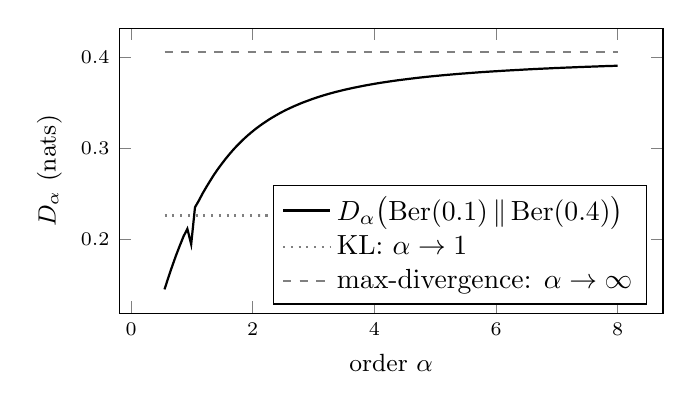
\begin{tikzpicture}
\begin{axis}[
  width=0.7\textwidth, height=5.2cm,
  xlabel={order $\alpha$}, ylabel={$D_\alpha$ (nats)},
  domain=0.55:8, samples=120,
  legend pos=south east, legend cell align=left,
  tick label style={font=\scriptsize}, label style={font=\small}
]
\addplot[black, thick]
  {ln(0.1^x * 0.4^(1-x) + 0.9^x * 0.6^(1-x))/(x-1)};
\addlegendentry{$D_\alpha\bigl(\mathrm{Ber}(0.1)\,\|\,\mathrm{Ber}(0.4)\bigr)$}
\addplot[gray, thick, dotted] {0*x + 0.2262};
\addlegendentry{KL: $\alpha \rightarrow 1$}
\addplot[gray, thick, dashed] {0*x + 0.4055};
\addlegendentry{max-divergence: $\alpha \rightarrow \infty$}
\end{axis}
\end{tikzpicture}
\caption{R\'enyi divergence vs.\ the order $\alpha$ for two Bernoulli distributions:
nondecreasing, through KL at $\alpha = 1$, converging to the max-divergence pure DP
bounds --- R\'enyi-DP certifies one point of this curve.}
\label{fig:inf-renyi}
\end{widefigure}

The last two rungs convert information into impossibility. First, incompressibility ---
the counting reading of Theorem~\ref{thm:inf-source}:

\begin{corollary}[Incompressibility]\label{cor:inf-counting}
If $X$ is uniform over $M$ outcomes then $H(X) = \log_2 M$, and any data structure
with $s$ bits that determines $X$ must satisfy $s \ge \log_2 M$: $s$ bits give fewer
than $2^s$ states, and each state witnesses only one $X$. \eop
\end{corollary}

\begin{proof}
Theorem~\ref{thm:inf-source} at the uniform distribution; the phrasing is pigeonhole.
\end{proof}

The method of \emph{incompressibility lower bounds} runs this backwards: too small a
sketch would be a code for objects of entropy beyond its bit count ---
Section~\ref{sec:inf-sublime} is a full exhibit. Second, Fano: an observation carrying
little information about a hypothesis pins down no estimator.

\begin{theorem}[Fano]\label{thm:inf-fano}
Let $X$ take $M \ge 2$ values, let $Y$ be generated through any channel from $X$, and
let $\hat X(Y)$ be any estimator. With $p_e = \Pr[\hat X(Y) \ne X]$,
\[
p_e \;\ge\; \frac{H(X \mid Y) - 1}{\log_2 M}. \eopm
\]
\end{theorem}

\begin{proof}[Proof sketch]
Condition on the error indicator $E = \mathbf{1}\{\hat X \ne X\}$: since $(X, E)$ is
determined by $(X, Y)$, $H(X|Y) \le H(E|Y) + H(X|E,Y) \le 1 + (1-p_e)\log_2 M$ ($E$
is binary; given $E = 0$, $X$ is determined by $Y$). Rearrange.
\end{proof}

\begin{corollary}[Capacity-style impossibility]\label{cor:inf-fano-cap}
If $X$ is uniform over $M$ hypotheses and the observable $Y$ satisfies $I(X;Y) =
\log_2 M - H(X|Y) \le c$, then every estimator errs with probability at least
$1 - (c+1)/\log_2 M$. \eop
\end{corollary}

\subsection{How to choose the information measure}
\label{sec:inf-choose}

The selection is mechanical once the deliverable is named. \emph{Space, communication,
or encoding bounds} ($\ge$ or $\approx$ bits): the source-coding pair
(Theorem~\ref{thm:inf-source}, Corollary~\ref{cor:inf-counting}) --- upper bounds by
exhibiting a code (Jensen bounds average code length), lower by incompressibility.
\emph{Distinguishability of two distributions} (privacy, testing, distributional
error): KL for expected-loss statements, R\'enyi $D_\alpha$ when stages compose ---
privacy accounting lives here, $\alpha$ tuned at the final conversion. \emph{Estimation
impossibility}: Fano (Theorem~\ref{thm:inf-fano}) with the capacity reading of
Corollary~\ref{cor:inf-fano-cap}. \emph{Structural size inequalities} (output sizes,
join costs): the Shannon-inequality system of Corollary~\ref{cor:inf-submodular},
optimized as a linear program.

\begin{reachbox}{When to Reach for Information Theory}
Reach when the claim is about \emph{information content} or
\emph{distinguishability} rather than average behavior: space lower bounds for
sketches, ``no mechanism can distinguish neighbors,'' ``no estimator recovers the
hidden data,'' ``this encoding is within $O(1)$ of optimal.'' Then run the recipe:
\begin{enumerate}
\item Name the random object: the stream prefix, the neighboring pair $(D, D')$, the
  hypothesis $X$ --- and what must be remembered, compared, or estimated about it.
\item Pick the measure: entropy for content (space/communication), KL for expected
  distributional error, R\'enyi $D_\alpha$ when stages compose (privacy accounting),
  Fano for estimation impossibility.
\item Write the chain-rule telescope along the structure: $H(X_1 \cdots X_k) = \sum_i
  H(X_i \mid \text{past})$, or the mixture decomposition over samples or stages.
\item Convert to the bound: $\mathbb{E}[\ell] \ge H$; $\operatorname{TV} \le
  \sqrt{D/2}$; $p_e \ge (H(X|Y)-1)/\log M$ (Fano); $\varepsilon' = \varepsilon +
  \ln(1/\delta)/(\alpha-1)$ (privacy conversion).
\end{enumerate}
\end{reachbox}

\section{Shannon inequalities as a join algorithm}
\label{sec:inf-panda}

The exemplar is a PODS'26 paper on join query processing \citep{sigmod26-185}\pods.
Evaluating conjunctive queries is the heart of database theory, and worst-case optimal
algorithms alone ignore the \emph{skew} real data exhibits: a degree constraint saying
``each value of $X$ has at most $N_{Y|X}$ matching $Y$s'' can shrink the output by
orders of magnitude. The PANDA framework exploits such constraints through the
polymatroid inequalities of Corollary~\ref{cor:inf-submodular}, but the original
algorithm pays for its generality with complex recursive partitioning. The paper
introduces \emph{PANDAExpress}: pick the inequality's weights by LP duality, and turn
each Shannon-inequality proof step into a recursive hyperplane partition of the data.
The result computes a query model meeting the polymatroid size bound $B$ in time
$O(N \log N + B \log N)$, recovering fractional hypertree-width and submodular-width
runtimes as corollaries.

\paragraph{Problem.}
Queries are \emph{disjunctive datalog rules} (DDRs)
\[
Q(Z) \;:\!-\; \bigvee_{R(X) \in \Sigma_{\mathrm{in}}} R(X)
\]
An output \emph{model} assigns tuples to the atoms
$Q(Z) \in \Sigma_{\mathrm{out}}$ so that every tuple $t$ of the natural join
$\Join_{\Sigma_{\mathrm{in}}}$ is covered, i.e.\ $t_Z \in Q(Z)$ for some $Z$; the goal
is a \emph{small} model. The instance satisfies \emph{degree constraints}
$(\Delta, N)$: for each term $\delta = (Y|X) \in \Delta$, the max degree
$\deg_R(Y|X{=}x)$ is at most $N_\delta$ in some input relation $R$. Writing $h$ for
the entropy function of any distribution consistent with the constraints, a
\emph{Shannon-flow inequality} is
\[
\sum_{Z \in \Sigma_{\mathrm{out}}} \lambda_Z\, h(Z) \;\le\;
\sum_{\delta \in \Delta} w_\delta\, h(\delta),
\qquad \| \lambda \|_1 = 1, \ \ \lambda, w \ge 0 \ \text{rational},
\]
valid for all polymatroids, where $h(Y|X) = h(XY) - h(X)$; it certifies
$|\Sigma_{\mathrm{out}}| \le B$ with $B = \prod_\delta N_\delta^{w_\delta}$ (take
logs of $h(\delta) \le \log N_\delta$).

\paragraph{Guarantee.}

\begin{theorem}[PANDAExpress, Theorem~6.4 of the paper]\label{thm:inf-panda-main}
Given a DDR, an input instance over $\Sigma_{\mathrm{in}}$ of size $N$ satisfying
degree constraints $(\Delta, N)$, and a Shannon-flow inequality with weights
$(\lambda, w)$, PANDAExpress computes a model $\Sigma_{\mathrm{out}}$ for the DDR of
size
\[
\|\Sigma_{\mathrm{out}}\| \;=\; O(B)
\quad\text{in time}\quad
O\bigl(N\log N + B\log N\bigr),
\qquad B \;=\; \prod_{\delta\in\Delta} N_\delta^{w_\delta}. \eopm
\]
\end{theorem}

\paragraph{How information theory is applied.}
Everything hangs on one move: the paper gives the Shannon inequality a
\emph{measure-theoretic} second life. A sub-probability measure is a nonnegative
function with total mass at most $1$; its marginals and conditionals are again such,
and so is the geometric mean of $k$ of them (AM--GM/H\"older on the masses). The
weights come first: LP duality (Proposition~6.3 of the paper) minimizes
$B = \prod_\delta N_\delta^{w_\delta}$ subject to the Shannon-flow inequality, and any
optimal solution puts $w_\delta = 0$ on every constraint with $N_\delta > B$: the
budget ignores loose constraints. The workhorse then converts the inequality into
measures: instantiate each constraint $\delta = (Y|X)$ on the data as
$p_\delta(y|x) = 1/N_\delta$ if $(x,y)$ occurs in some input relation, $0$ otherwise
--- a sub-probability conditional.

\begin{lemma}[Measures from inequalities; Lemma~4.4 of the paper, notation cleaned]
\label{lem:inf-panda-measures}
Let $(\lambda, w)$, $\|\lambda\|_1 = 1$, be nonnegative rational weights for which
$\sum_Z \lambda_Z h(Z) \le \sum_\delta w_\delta h(\delta)$ is a Shannon-flow inequality
over $V$. Then for any collection of sub-probability measures $p_\delta$, $\delta \in
\Delta$, there exist sub-probability measures $p_Z$, $Z \in \Sigma_{\mathrm{out}}$,
such that
\[
\prod_{Z \in \Sigma_{\mathrm{out}}} p_Z(t)^{\lambda_Z} \;\ge\;
\prod_{\delta \in \Delta} p_\delta(t)^{w_\delta}
\qquad \text{for all } t \in \mathrm{Dom}_V. \eopm
\]
\end{lemma}

\begin{proof}[Proof sketch]
Clear denominators to an \emph{integral} Shannon-flow inequality over multisets; it
has a \emph{proof sequence} (Theorem~2.4 of the paper): single steps of submodularity,
composition, decomposition, or monotonicity. Give each term of $\mathcal{D}$ its
measure; at every step replace measures so the pointwise product only grows:
monotonicity $h(XY) \to h(X)$ replaces $p_{XY}$ by its marginal; submodularity
$h(Y|X) \to h(Y|XZ)$ re-conditions, $p_{Y|XZ}(y|xz) := p_{Y|X}(y|x)$; composition and
decomposition split $p_{XY} = p_X \cdot p_{Y|X}$ or merge back. The final multiset
contains $\mathcal{Z}$; group equal terms by geometric means (still sub-probability)
and normalize exponents back to $(\lambda, w)$. Full case analysis in
Section~\ref{sec:inf-appendix}.
\end{proof}

The bound follows by ``taking logs'': for a join tuple $t \in
\Join_{\Sigma_{\mathrm{in}}}$, every $p_\delta(t) = 1/N_\delta$, so the right-hand
product is $1/B$; since $\|\lambda\|_1 = 1$, some $Z$ has $p_Z(t_Z) \ge 1/B$, and the
model $Q(Z) = \{z : p_Z(z) \ge 1/B\}$ covers every join tuple and has at most $B$
tuples because $p_Z$ has mass $\le 1$ --- Markov at the measure level.
\sidenote{Why \emph{hyperplanes}: no axis-parallel light/heavy split proves one
two-atom cover, but the tilted hyperplane $h(C) = h(F)$ does; the geometric-mean
construction finds such cuts automatically.} The algorithm
implements each proof step as a recursive partition along the step's measure threshold
(light tuples continue the proof sequence; the heavy side restarts via the paper's
Reset Lemma), and a potential $|\mathcal{D}| + |\mathcal{M}| + 3|\mathcal{S}|$
decreases at every restart, bounding the recursion depth by the proof length.

\paragraph{What it buys.}
Worst-case-optimal evaluation \emph{with} skew at $O(N\log N + B\log N)$, where prior
PANDA-style algorithms needed many bucket partitions per cut --- and the theory
delivers the algorithm, not just the bound: each proof step is executable.

\section{R\'enyi-divergence accounting for sampled private queries}
\label{sec:inf-s4s}

The exemplar is a SIGMOD'26 paper on private query processing \citep{sigmod26-079}.
Answering select--join--aggregate (SJA) queries under \emph{user-level} differential
privacy --- no adversary may confidently infer the presence or absence of any one
\emph{user's} entire tuple set --- is demanding, because users contribute unboundedly
many tuples and one heavy user can dominate the answer, and the state of the art
attains strong accuracy only via expensive optimization over the whole database. The
paper's engine, DP-S4S, accelerates the search by Poisson-sampling tuples before
privatizing, truncates each heavy user's contribution at a threshold found privately
by a sparse-vector-technique (SVT) search, and releases through a smooth-sensitivity
Gaussian mechanism. Its privacy analysis is pure
information theory: privacy \emph{is} a divergence bound between neighboring outputs,
sampling turns each output into a \emph{mixture} over samples, and the divergence of
mixtures is controlled by R\'enyi quasi-convexity, with a binomial count deciding
which components matter.

\paragraph{Problem.}
Privacy of a mechanism $M$ is a bound on how distinguishable $M(D)$ and $M(D')$ are for
\emph{neighboring} inputs $D \sim D'$ (user-level: all tuples of one user added or
removed). The information-theoretic formulation used here is R\'enyi differential
privacy \citep{information-theory-bg5}:

\begin{definition}[R\'enyi DP, user level]\label{def:inf-rdp}
For $\alpha > 1$ and $\varepsilon > 0$, a randomized mechanism $M$ is
$(\alpha, \varepsilon)$-RDP if for all neighboring $D, D'$,
\[
D_\alpha\bigl(M(D) \,\big\|\, M(D')\bigr) \;\le\; \varepsilon,
\]
with $D_\alpha$ as in Definition~\ref{def:inf-renyi}. An $(\infty, \varepsilon)$
bound is pure $\varepsilon$-DP; RDP converts back to
$(\varepsilon + \frac{\ln(1/\delta)}{\alpha - 1},\, \delta)$-DP for any $\delta > 0$.
\end{definition}

The engine Poisson-samples each tuple independently with probability $q$ (sample
$S \subset T$), runs an SVT search $M_1$ over truncation thresholds on $S$, and
releases the truncated aggregate through a Gaussian mechanism $M_2$ calibrated in
R\'enyi terms. The pipeline is $L = \ell + 1$ stages ($\ell$ SVT iterations plus the
release), each needing an amplified budget: sampling shrinks the effective
divergence, and the analysis must say by how much.

\paragraph{Guarantee.}

\begin{corollary}[RDP-S4S for scalar SJA; Corollary of the paper, notation cleaned]
\label{cor:inf-s4s-rdp}
There is an $(\alpha, \varepsilon)$-RDP version of the engine's main algorithm. Let $n$
be the number of records, $m$ the number of users, $q$ the sample rate,
$\tau^*(T) = \max_u \sum_{t \in T}\mathbf{1}[u \prec t]$ the maximum per-user
contribution, and $\varepsilon_i^* \ge \varepsilon/(\ell+1)$ the amplified
noise-calibration budget. With probability $1 - \beta$,
\[
\bigl|\hat f(T) - f(T)\bigr|
\;=\; O\Bigl(\sqrt{\tfrac{n}{q}} + \tfrac{1}{q} +
\frac{\sqrt{\alpha}}{\varepsilon_i^*}\Bigl(\tau^*(T) + \sqrt{\tfrac{\tau^*(T)}{q}}\Bigr)\Bigr),
\]
where $O(\cdot)$ hides constants and polylogarithmic factors in $m$ and $1/\beta$. \eop
\end{corollary}

\paragraph{How information theory is applied.}
The random object is the pair of \emph{output distributions on neighboring inputs} ---
and sampling makes each a mixture:
$\Pr[M(T) = z] = \sum_S \Pr[\lambda(T){=}S]\cdot\Pr[M(S) = z]$. Quasi-convexity
(Lemma~\ref{lem:inf-quasiconvex}) bounds the mixture's divergence by the worst
component, $D_\alpha\bigl(\sum_S p_S M(S) \,\|\, \sum_S p_S M(S \cup S_u)\bigr) \le
\max_S D_\alpha(M(S) \| M(S \cup S_u))$; the reverse direction uses convexity in the
second argument plus concavity of $\ln$ (the Proposition~\ref{prop:inf-klmix} logic,
order by order). The per-component divergence is Gaussian, closed-form:

\begin{lemma}[Gaussian R\'enyi divergence; Lemma of the paper, notation cleaned]
\label{lem:inf-gauss-renyi}
For $\mu_1, \mu_2 \in \mathbb{R}^d$ and i.i.d.\ noise,
\begin{align*}
D_\alpha\bigl(\mathcal{N}(\mu_1, \sigma_1^2 I_d) \,\|\, \mathcal{N}(\mu_2, \sigma_2^2
I_d)\bigr)
\;&=\; \frac{\alpha \,\|\mu_1 - \mu_2\|_2^2}{2\sigma^2_\mathrm{mix}}\\
\;&+\; \frac{d}{2}\,(\alpha - 1)\,
\ln \frac{\sigma_1^{\,2(1-\alpha)}\,\sigma_2^{\,2\alpha}}{\sigma^2_\mathrm{mix}},
\eopm
\end{align*}
where $\sigma^2_\mathrm{mix} = (1-\alpha)\sigma_1^2 + \alpha\sigma_2^2$; the
divergence is infinite if $\sigma^2_\mathrm{mix} \le 0$. For equal scales $\sigma$,
only the first term survives: $D_\alpha = \alpha\|\mu_1 - \mu_2\|_2^2 / 2\sigma^2$.
\end{lemma}

The count structure now enters: user $u$ contributes $k$ of its $\hat\tau$ sampled
tuples to $S \cup S_u$ with probability $p_k = \Pr[\mathrm{Bin}(\hat\tau, q) = k]$, and
the truncated query moves by at most $\min\{\tau, k\}$ between components --- the
amplified budget is a binomial average of per-count Gaussian divergences,
$\varepsilon'(\alpha) = \frac{1}{\alpha-1}\ln\bigl(\sum_{k \le \hat\tau} p_k
\exp((\alpha-1)\, c\,\min\{\tau,k\}^2) + \Pr[\mathrm{Bin}(\hat\tau,q) > \hat\tau]\,
e^{(\alpha-1)\varepsilon_s}\bigr)$ with $c$ set by the noise scale (``RDP
Amplification'' Lemma of the paper; some symbols dropped by the extractor, structure
preserved). In the pure-DP limit this yields
$\varepsilon' = \ln\bigl(1 + q'(e^{\varepsilon_1} - 1)\bigr)$ with
$q' = 1 - (1-q)^{\hat\tau}$ --- subsampling amplification with the collision
probability $q'$ in place of $q$. Finally the stages compose: RDP composition sums the
$L$ budgets (Proposition~\ref{prop:inf-renyicalc}), and Definition~\ref{def:inf-rdp}'s
conversion returns to $(\varepsilon, \delta)$-DP, $\alpha$ chosen once to optimize the
final $\varepsilon$.

\paragraph{What it buys.}
User-level privacy whose accounting survives $L$-stage composition without the
$\sqrt{L}$ loss of naive advanced composition, sampling amplification recognized as a
divergence shrink, and --- via the $\sqrt{\alpha}$ term in
Corollary~\ref{cor:inf-s4s-rdp} --- a dial trading R\'enyi order against noise scale.

\section[Source coding for expandable sketches]{Source coding and incompressibility for expandable sketches}
\label{sec:inf-sublime}

The exemplar is a SIGMOD'26 paper on streaming frequency estimation
\citep{sigmod26-231}, read here through the entropy lens rather than the estimator
lens of Chapter~\ref{ch:est}. Frequency-estimation (FE) sketches such as Count-Min and
CountSketch commit to a fixed width at construction, but real streams are unbounded
and skewed: the length is unknown in advance, heavy keys make some counters grow
large while most stay tiny. The paper's system, \emph{Sublime}, is an expandable
CountSketch-style sketch that grows with the stream, and its two-sided theory is a
textbook information argument. Upper bound, source coding: counters are stored as
short stubs plus rare extensions, and Jensen (concavity of $\log$) shows the array
encodes in about $w \log_2(k/w) + O(w)$ bits --- within a constant of the information
content of $w$ counters summing to $k$. Lower bound, incompressibility: any FE sketch
achieving error $E(N)$ at confidence $1-\delta$ on growing streams must at some point
hold at least $\frac{N}{E(N)}\bigl[\Omega(\log \frac1\delta +
\log\log\frac{N}{E(N)}) - \Theta(1)\bigr]$ bits, else its state would compress random
key sequences below their entropy.

\paragraph{Problem.}
A stream of keys (insertions, deletions) of unknown ultimate length $N$ is processed
by an \emph{expandable} FE sketch maintaining $d$ counter arrays whose width follows a
size function $W(\cdot)$ --- e.g.\ $W(N) = N/\varepsilon$ or $W(N) =
N^\alpha/\varepsilon$ with $0 \le \alpha < 1$ --- expanding over \emph{epochs} at
width $W_j = W(N_j)$. Skew makes the counter values far from uniform: a few large,
many small, and the storage cost depends on how compactly that multiset is
\emph{written down}. The lower-bound adversary is any FE sketch with only
overestimation errors guaranteeing error $E(N)$ at confidence $1-\delta$ on a
growing stream.

\paragraph{Guarantee.}

\begin{theorem}[Memory footprint; Theorem of the paper, notation cleaned]
\label{thm:inf-sublime-space}
With a sublinear power size function, the sketch's memory footprint is
\[
\approx \;d \cdot W(N) \cdot \bigl[4.41 + 1.26\cdot \log_2 \tfrac{N}{W(N)}\bigr]
\ \text{bits};
\]
with a linear size function, $\approx d \cdot W(N) \cdot [4.41 + 1.26\log_2
\frac{N\log_2 N}{W(N)}]$. The same bounds hold with $W(F)$ (the squared $\ell_2$ norm)
in place of $W(N)$, plus one bit per counter if counters are signed. \eop
\end{theorem}

\begin{theorem}[Space lower bound; Theorem of the paper]\label{thm:inf-sublime-lb}
Any FE sketch with only overestimation errors that processes growing streams with error
bound $E(N)$ and confidence $1-\delta$ must use at least
\[
\frac{N}{E(N)}\cdot\Bigl[\Omega\Bigl(\log\tfrac{1}{\delta} +
\log\log\tfrac{N}{E(N)}\Bigr) - \Theta(1)\Bigr] \eopm
\]
bits of memory at some point in time while processing a stream.
\end{theorem}

\paragraph{How information theory is applied.}
The upper bound runs the source-coding direction of Theorem~\ref{thm:inf-source}. A
single counter value $v$ is coded as an $s$-bit \emph{stub} plus, when $v \ge 2^s$, a
variable-length \emph{extension} of $\lfloor v/2^s \rfloor$ in base $3$ --- at most
$4 + 1.26\log_2 v$ bits in total (Lemma of the paper; the constant $1.26 =
2\log_3 2$ is the base conversion). The array-level step is the entropy-flavored one:

\begin{lemma}[Counter-array encoding; Lemma of the paper, notation cleaned]
\label{lem:inf-sublime-array}
An array of $w$ unsigned counters with total absolute value $k$ encodes in
\[
w\cdot\bigl[4.41 + 1.26\cdot\log_2 (k/w)\bigr] \ \text{bits}, \eopm
\]
and signed counters cost one extra bit each.
\end{lemma}

\begin{proof}[Proof sketch]
Sum the per-counter bound and use the concavity of $\log_2$ \emph{twice}: the stub
length satisfies $s \le 2 + \frac1w\sum_i \log_2|v_i| \le 2 + \log_2(k/w)$ (Jensen),
and after replacing each per-counter term by the larger of the two scales,
$\sum_i \log_2(\frac{k}{4w} + |v_i|) \le w\log_2(\frac54 \cdot \frac kw)$ (Jensen
again); $1.26\log_2\frac54 \approx 0.41$ supplies the constant. Full proof in
Section~\ref{sec:inf-appendix}.
\end{proof}

The lower bound runs the converse, Corollary~\ref{cor:inf-counting}, as a
\emph{reduction to compression}: a smaller sketch would compress sequences $\bar x =
(x_1, \dots, x_n)$ of $n = N/(2E(N))$ keys drawn uniformly from a universe of size
$u \cdot n$ --- objects of entropy $n\log_2(un)$. Three steps. First, a
\emph{variance chain rule} (law of total variance over the sketch's estimates across
prefixes $\bar x_1, \dots, \bar x_\ell$ of geometrically growing lengths) exhibits
one prefix state $\mathcal{S}^*_i$ whose estimates have second moment at most
$2V/\log_2 n$. Second, \emph{fixing the internal randomness}: averaging over the seed
makes bias and variance small simultaneously, so one seed works on at least half of
all sequences --- a seed with $\mu(\bar x) \le 64\delta/\log_2 n$ and $\nu(\bar x)
\le 64\delta/\log_2 n$ on at least half the sequences (Lemma of the paper). Third,
the \emph{code}: write $\bar x$ as (seed, state of $\mathcal{S}^*_i$); a decoder
re-queries the sketch for every key and recovers $\bar x$ up to the error event, so
the codewords are nearly injective over half of a set of entropy $n\log_2(un)$. The
state must hold $n\log_2(un) - O(n \cdot E(N))$ bits minus the seed index, which
unwinds to the stated $\frac{N}{E(N)}[\log \frac1\delta + \log\log \frac{N}{E(N)} -
\Theta(1)]$: a sketch that answers queries is a code.

\paragraph{What it buys.}
A footprint certified \emph{while it grows} --- no prior knowledge of stream length
or skew --- within a small logarithmic factor of what any expandable FE sketch must
pay; the same entropy accounting compresses its counters and fences off its
competition.

\section{Divergence budgets for private data synthesis}
\label{sec:inf-dpsynth}

The exemplar is a SIGMOD'26 Experiments \& Analysis paper benchmarking differentially
private tabular data synthesis \citep{sigmod26-279}. A DP synthesizer generates a fake
table preserving useful statistics of a real one while protecting every individual's
row; synthesizers are pipelines --- select marginals, discretize, infuse noise,
compose the joint --- and competing systems make incomparable accuracy/privacy
choices, so evaluations are hard to interpret. The paper benchmarks representative
synthesizers under a unified treatment: every stage's privacy loss is an
$(\alpha, \varepsilon)$-RDP budget, stages compose additively, and accuracy is the
\emph{KL divergence} between synthesized and true joint. Its theory contribution is
an ordering theorem: estimating a joint through noisy \emph{conditionals} is never
worse in KL error than a \emph{product of noisy marginals} --- the divergence version
of ``conditionals carry the dependence.'' The extract records the statements without
proofs; we transcribe conservatively and flag where the standard argument fills in.

\paragraph{Problem.}
The pipeline is a composition of randomized stages over a table with attributes
$A_1, \dots, A_d$: per-attribute marginals are estimated noisily (Gaussian mechanism,
exponential mechanism for selection, PrivTree partitions, rare-value merges), and the
joint is then \emph{estimated} from the noisy pieces --- either \emph{independently},
as the product $\hat P[A_i]\cdot\hat P[A_j]$ of noisy marginals, or
\emph{conditionally}, through noisy conditionals. Each stage $j$ carries an
$(\alpha, \varepsilon_j)$-RDP guarantee (Definition~\ref{def:inf-rdp}), so the
composed synthesizer is $(\alpha, \sum_j \varepsilon_j)$-RDP by composition and
converts to $(\varepsilon, \delta)$-DP at the end; accuracy is
$D\bigl(\hat P[A_i, A_j] \,\|\, P[A_i, A_j]\bigr)$, the KL error of the implied
two-attribute joint against the true one.

\paragraph{Guarantee.}

\begin{theorem}[Estimation ordering; Theorem of the paper, notation cleaned]
\label{thm:inf-dpsynth-order}
For any pair of attributes $(A_i, A_j)$, the KL-divergence error of conditional
estimation is always no larger than that of independent estimation:
\[
D\bigl(\hat P_{\mathrm{c}}[A_i, A_j] \,\big\|\, P[A_i, A_j]\bigr)
\;\le\;
D\bigl(\hat P_{\mathrm{i}}[A_i, A_j] \,\big\|\, P[A_i, A_j]\bigr),
\]
where $\hat P_{\mathrm{c}}$ is the joint estimated through the noisy conditionals and
$\hat P_{\mathrm{i}} = \hat P[A_i]\cdot \hat P[A_j]$ is the product of the noisy
marginals (the paper's display is partially mangled by extraction; the ordering claim
and both comparands are as stated). \eop
\end{theorem}

\paragraph{How information theory is applied.}
The workhorse is the mixture/conditional convexity of KL --- Proposition~\ref{prop:inf-klmix}
specialized, and transcribed by the paper as a standalone lemma:

\begin{lemma}[KL convexity; Lemma of the paper, notation cleaned]\label{lem:inf-dpsynth-convex}
If $P_1(z) = \sum_x p(x)\,P_1(z \mid x)$ and $P_2(z) = \sum_x p(x)\,P_2(z \mid x)$ share
the same mixing weights, then
\[
D\bigl(P_1(z) \,\|\, P_2(z)\bigr)
\;\le\; \sum_x p(x)\, D\bigl(P_1(z \mid x) \,\|\, P_2(z \mid x)\bigr). \eopm
\]
\end{lemma}

\begin{proof}[Proof sketch]
Proposition~\ref{prop:inf-klmix}(ii) with $z$ marginalized away: the joint divergence
over $(x, z)$ equals the average of the conditional divergences (the mixing weights
coincide), and marginalizing $x$ is data processing, which cannot increase
divergence.
\end{proof}

Applied with $x$ ranging over the values of $A_i$, the lemma converts the joint error
of the conditional estimator into the \emph{average of its per-condition errors};
comparing term by term against the error the product estimator pays for the same
marginals yields the ordering of Theorem~\ref{thm:inf-dpsynth-order} --- noise spent
inside conditionals is never wasted, noise spent pretending independence is. The
privacy side is divergence budgeting: each stage comes with a tabulated RDP guarantee
--- the Gaussian mechanism $(\alpha, \alpha \Delta_2^2/2\sigma^2)$-RDP at noise scale
$\sigma$, the exponential mechanism $(\alpha, \alpha\varepsilon^2/8)$, rare-value
merge $(\alpha, \alpha\Delta_2^2)$, PrivTree $(\alpha, \alpha\Delta_1)$ (statements of
the paper, imported from prior work; $\Delta_p$ the $\ell_p$ sensitivity) --- and the
total budget $\sum_j \varepsilon_j$ is what the benchmark allocates across stages
before converting once to $(\varepsilon, \delta)$-DP. The extract records no proofs
for these; they are standard in the RDP literature \citep{information-theory-bg5}.

\paragraph{What it buys.}
An apples-to-apples budget grammar --- any synthesizer is a diversion of one
$\sum_j \varepsilon_j$ across stages --- and a provable design rule: spend noise on
conditional structure; Theorem~\ref{thm:inf-dpsynth-order} certifies it never loses
KL accuracy against independence.

\section{Advanced usage and further reading}
\label{sec:inf-advanced}

The corpus's fifth paper uses entropy as a difficulty measure, not a bound.

\paragraph{Entropy as difficulty: LM-approximated LIKE predicates
\citep{sigmod26-237}.}
SQL \texttt{LIKE} patterns (wildcard string matching) are costly to evaluate at
scale, and language models suggest a shortcut: let the model approximate the
predicate --- when is that viable? The paper models a pattern's difficulty by its
\emph{entropy}: Theorem~5.1 of the paper computes $H(P)$ for a \texttt{LIKE} pattern
with $p$ underscore and $q$ percent wildcards over alphabet $\Sigma$ --- the
underscores each contribute $\ln|\Sigma|$, the percents a combinatorial sum over the
extra lengths they admit (the extract's formula is partially mangled; the quantity is
the logarithm of the number of strings the pattern generates, the pattern's intrinsic
uncertainty). The success model is a capacity ratio: a model with abstract capacity
$M$ internalizes task $W$ with probability at least $c\cdot\min\{1, M/H(W)\}$ --- the
model must overwhelm the task's entropy, the same $M$ versus
$\log_2(\text{hypotheses})$ comparison Fano turns into impossibility, here read
optimistically as a gate: LM approximation is worth trying exactly when the
predicate's entropy fits the model's capacity. The framework is heuristic (capacity
is assumed, not derived) --- the corpus's cleanest entropy-as-\emph{predictor} use.

\subsection{Further reading}

\begin{itemize}
\item Cover and Thomas \citep{information-theory-bg2} --- the standard textbook:
  entropy, source coding, chain rules, KL, and the inequalities used here.
\item Shannon \citep{information-theory-bg1} --- the original: the source-coding
  theorem and the entropy calculus in their first form.
\item R\'enyi \citep{information-theory-bg3} --- the 1961 paper introducing the
  order-$\alpha$ divergences privacy accounting runs on.
\item van Erven and Harremo\"es \citep{information-theory-bg4} --- the modern
  treatment of R\'enyi divergence: monotonicity, quasi-convexity, conversions.
\item Mironov \citep{information-theory-bg5} --- R\'enyi differential privacy: the
  composition calculus both privacy exemplars run on.
\item Fano \citep{information-theory-bg6} and Pinsker \citep{information-theory-bg7}
  --- the originals behind Theorems~\ref{thm:inf-fano} and~\ref{thm:inf-pinsker}.
\item Yeung \citep{information-theory-bg8} --- entropy functions and polymatroids,
  and the Shannon-type vs.\ entropic gap behind Section~\ref{sec:inf-panda}.
\end{itemize}

\begin{recap}
\item \textbf{What the tool is.} Information-theoretic arguments bound information
  content (entropy, bits) and distinguishability (KL/R\'enyi divergence), in both
  directions: $H$ bits guarantees an $\approx H$-bit encoding and forbids anything
  smaller.
\item \textbf{Which measure when.} Space/communication: entropy and source coding
  (upper by exhibiting codes, lower by incompressibility). Distributional error: KL.
  Composed stages and privacy: R\'enyi $D_\alpha$ --- quasi-convex over mixtures,
  additive over stages, converted once at the end. Impossibility: Fano, capacity
  reading. Structural sizes: Shannon inequalities, optimized by LP duality.
\item \textbf{Why it works.} Every rung telescopes: a chain rule (entropy, variance,
  or divergence over mixtures) decomposes the object along the pipeline, and Gibbs
  ($D \ge 0$) turns the telescope into a one-sided bound.
\item \textbf{What the corpus showed.} PANDAExpress (Section~\ref{sec:inf-panda}):
  Shannon inequalities re-proved as sub-probability measures, each proof step an
  executable hyperplane partition. DP-S4S (Section~\ref{sec:inf-s4s}): privacy as
  R\'enyi divergence, sampling as mixtures tamed by quasi-convexity. Sublime
  (Section~\ref{sec:inf-sublime}): counters encoded to $w[4.41 + 1.26\log_2(k/w)]$
  bits; any expandable sketch forced to
  $\frac{N}{E(N)}[\log\frac1\delta + \log\log\frac{N}{E(N)} - \Theta(1)]$. DP
  synthesis (Section~\ref{sec:inf-dpsynth}): KL convexity orders conditional over
  independent estimation; RDP assigns per-stage budgets.
\item \textbf{Advanced usage.} Entropy as a difficulty measure and capacity gate for
  LM-approximated predicates (Section~\ref{sec:inf-advanced}); deferred proofs in the
  Appendix (Section~\ref{sec:inf-appendix}).
\end{recap}

\section{Appendix}
\label{sec:inf-appendix}

Proofs omitted from the main text are collected here.

\subsubsection*{Proof of Lemma~\ref{lem:inf-panda-measures} (PANDA measures)}
{\itshape Statement (recalled).} A Shannon-flow inequality with rational weights
$(\lambda, w)$, $\|\lambda\|_1 = 1$, converts any sub-probability measures $p_\delta$
into $p_Z$ with $\prod_Z p_Z^{\lambda_Z} \ge \prod_\delta p_\delta^{w_\delta}$.\eop

\begin{proof}
Write $\lambda_Z = m_Z/d$, $w_\delta = m_\delta/d$ with positive integers $m_Z,
m_\delta$ and common denominator $d$, and multiply through: an \emph{integral}
Shannon-flow inequality over multisets, $Z$ appearing $m_Z$ times and $\delta$
appearing $m_\delta$ times. By the proof-sequence construction (Theorem~2.4 of the
paper) it is proved by steps turning $\sum_{\delta \in \mathcal{D}_i} h(\delta)$ into
$\sum_{\delta \in \mathcal{D}_{i+1}} h(\delta)$; we carry measures along so that
products only grow. Monotonicity $h(XY) \to h(X)$: replace $p_{XY}$ by its marginal;
then $p_{XY}(x,y) \le p_X(x)$ pointwise. Submodularity $h(Y|X) \to h(Y|XZ)$: set
$p_{Y|XZ}(y|xz) := p_{Y|X}(y|x)$; unchanged. Composition $h(X) + h(Y|X) \to h(XY)$:
set $p_{XY}(x,y) := p_X(x)\,p_{Y|X}(y|x)$; unchanged. Decomposition is the reverse
factorization via marginal and conditional; unchanged. Marginals and products of
sub-probability measures are sub-probability, so every output is legal. The final
multiset satisfies $\mathcal{D}_k \supseteq \mathcal{Z}$, so
$\prod_{Z \in \mathcal{Z}} p_Z(t) \ge \prod_{\delta \in \mathcal{D}}
p_\delta(t)^{m_\delta}$. Group the copies of each $Z \in \Sigma_{\mathrm{out}}$ by the
geometric mean $p_Z^{\mathrm{gm}} := \bigl(\prod_{\text{copies}} p_Z\bigr)^{1/m_Z}$:
it is sub-probability because, by H\"older and $\sum_x p_Z(x) \le 1$ per copy,
$\sum_x p_Z^{\mathrm{gm}}(x) \le \prod_{\text{copies}} \bigl(\sum_x p_Z(x)\bigr)^{1/m_Z}
\le 1$. Dividing all exponents by $d$ gives the claimed $(\lambda, w)$ form.
\end{proof}

\subsubsection*{Proof of Lemma~\ref{lem:inf-sublime-array} (counter-array encoding)}
{\itshape Statement (recalled).} An array of $w$ unsigned counters with total absolute
value $k$ encodes in $w\,[4.41 + 1.26\log_2(k/w)]$ bits.\eop

\begin{proof}
Per counter: values $v < 2^s$ occupy their $s$-bit stub; otherwise the stub keeps the
$s$ low-order bits and an extension codes $\lfloor v/2^s\rfloor$ in base $3$ with
$\log_3(v/2^s) + 2$ fragments of $2$ bits, for at most
$2(\log_3 2 \cdot \log_2(v/2^s) + 2) + s \le 4 + 1.26\log_2 v$ bits. Summing, $m \le
\sum_i \max(s,\, 4 + 1.26\log_2|v_i|)$. Tune the stub to the average counter: by
Jensen ($\log_2$ concave), $\frac1w\sum_i \log_2|v_i| \le \log_2(k/w)$, so
$s \le 2 + \log_2(k/w) = 4 + \log_2(k/4w)$. Each per-counter maximum is at most
$4 + 1.26\log_2(k/(4w) + |v_i|)$ (the max of two scales is bounded by the log of
their sum), and Jensen again gives
\[
\frac{1}{w}\sum_i \log_2\bigl(\tfrac{k}{4w} + |v_i|\bigr)
\;\le\; \log_2\Bigl(\tfrac{k}{4w} + \tfrac{k}{w}\Bigr)
\;=\; \log_2\bigl(\tfrac54\cdot\tfrac kw\bigr).
\]
Hence $m \le w[4 + 1.26\log_2(\frac54 \frac kw)] \le w[4.41 + 1.26\log_2(k/w)]$
since $1.26\log_2\frac54 \approx 0.41$.
\end{proof}

\bibliographystyle{plainnat}
\bibliography{chapters/information-theory-all}

\chapter{Communication Complexity}
\setcounter{section}{-1}   % sections start at 7.0 (see main.tex comment)
\label{ch:cc}

% ROLLOUT STUB (round 6) -- being written to the pilot spec (CHAPTER-RULES.md).
% Exemplars per plan.json: 115, 243, 357, 070 (PODS cap: two for this chapter).
This chapter is being revised; see Chapter~\ref{ch:intro} for the survey
context in the meantime.

\chapter{Online decision-making: competitive analysis and regret}

Online decision theory enters this corpus through systems doors: when to adapt a filter to a recurring false positive, whether to trust an ML oracle's prediction, how to clean a time series that has not yet arrived, how to tune a discretization knob. Four papers carry it---two via \emph{competitive analysis} \cite{sigmod26-242,sigmod26-094}, two via \emph{regret} \cite{sigmod26-140,sigmod26-221}, none an online-algorithms paper per se. They share one shape: the system commits to decisions while the input's future is unknown, and the committed sequence is judged against a hindsight optimum that sees everything. Two classical yardsticks quantify that gap, and choosing between them is this chapter's lesson.

\section{The tools}

\begin{definition}[Competitive ratio]
An online algorithm $A$ for a cost-minimization problem is \emph{$c$-competitive} if there is a constant $b$ such that
\[
\operatorname{cost}_A(\sigma) \;\le\; c\cdot\operatorname{cost}_{\mathrm{OPT}}(\sigma) + b
\qquad\text{for every input sequence }\sigma,
\]
where $\mathrm{OPT}$ is the offline optimum that observes all of $\sigma$---including where it ends---before acting.
\end{definition}

The canonical micro-example is \emph{ski rental}: skis rent for $1$ per day and cost $B$ to buy; each morning the skier learns only whether the season continues. Renting for $B$ days and then buying is $2$-competitive, and no deterministic algorithm does better; randomization lowers the barrier to $e/(e-1)\approx 1.58$ against an oblivious adversary~\cite{online-decisions-bg2}. The framework descends from the amortized analysis of list update and paging~\cite{online-decisions-bg1}. Figure~\ref{fig:ski-rental} shows the geometry; the memoryless ``when do I commit?'' structure is why this toy model reappears below in database clothing.

\begin{figure}[ht]
\centering
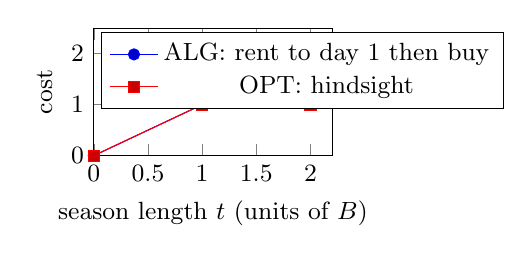
\begin{tikzpicture}
\begin{axis}[width=0.38\textwidth,height=3.2cm,
  xlabel={season length $t$ (units of $B$)}, ylabel={cost},
  xmin=0,xmax=2.2,ymin=0,ymax=2.5,
  legend pos=north west,legend style={font=\small},
  tick label style={font=\small},label style={font=\small}]
\addplot coordinates {(0,0) (1,1) (2,2)};
\addplot coordinates {(0,0) (1,1) (2,1)};
\legend{ALG: rent to day $1$ then buy,OPT: hindsight}
\end{axis}
\end{tikzpicture}
\caption{Ski rental with rent $1$ and buy price $B=1$: rent-to-$B$-then-buy matches OPT while $t<B$ and never exceeds $2\cdot\mathrm{OPT}$.}
\label{fig:ski-rental}
\end{figure}

\begin{definition}[Regret]
For decisions $a_1,\dots,a_T$, where round $t$ charges a loss $\ell_t(a_t)$ revealed only after the decision, the \emph{regret} against the best fixed comparator is
\[
R_T \;=\; \sum_{t=1}^{T}\ell_t(a_t)\;-\;\min_{a\in\mathcal{A}}\sum_{t=1}^{T}\ell_t(a).
\]
An algorithm is \emph{no-regret} if $R_T=o(T)$: its average loss converges to that of the best action chosen once, in hindsight.
\end{definition}

In the stochastic multi-armed bandit ($K$ actions, rewards in $[0,1]$ with fixed unknown means, only the chosen arm's reward observed), UCB plays the arm with the highest optimism index $\bar r_k+\sqrt{2\ln t/n_k}$ and achieves $R_T=O(\sqrt{KT\log T})$~\cite{online-decisions-bg3}; adversarial and unified views are surveyed in~\cite{online-decisions-bg4}. In short: the \emph{competitive ratio} prices the unknown future---unrestricted adversary, switching comparator, guarantee on every input---for one-shot commitments under adversarial workloads; \emph{regret} prices ignorance of a distribution---repeated rounds, per-round feedback, fixed comparator, $O(\sqrt{T})$ bound---for stochastic tuning loops.

\section{Four exemplars from the corpus}

\subsection{Ski rental inside a sketch filter}

A streaming distinct-count filter occasionally yields a false positive; each repeat costs a database lookup $C_{DB}$, adapting the entry costs an extra reverse-map lookup $C_{RM}=\alpha\,C_{DB}$, and after adapting both costs stop. Whether and when to adapt is ski rental in disguise---rental price $C_{DB}$, purchase price $C_{DB}+C_{RM}$, adversarial arrival stream.

\begin{theorem}[Adapt after $\lfloor\alpha\rfloor$ repeats; 2-competitive]
If $\alpha\ge 1$, i.e., the cost of querying the reverse map is greater than a database lookup, the optimal deterministic strategy is to adapt immediately after the false positive repeats $\lfloor\alpha\rfloor$ times, and is 2-competitive.
\end{theorem}

\begin{remark}[The golden-ratio threshold]
For $\alpha<1$ the two candidate policies have ratios $1+\alpha$ (adapt immediately) and $(2+\alpha)/(1+\alpha)$ (adapt on the second false positive); these cross where $\alpha^2+\alpha-1=0$, i.e.\ at $\alpha=(\sqrt{5}-1)/2\approx 0.618$. The optimal rule: adapt immediately when $\alpha<0.618$, adapt on the second occurrence otherwise.
\end{remark}

The competitive ratio is the right yardstick: the arrival stream is adversarial and the offline comparator knows when the repeats end. The skeleton also composes---augmenting a strongly adaptive filter with this routine bounds false positives by $(1+\lceil\alpha\rceil)\bigl(n\epsilon+O(\sqrt{n\epsilon\log n+\log n})\bigr)$ with high probability, the 2-competitive core living inside a high-probability bound. \cite{sigmod26-242}

\subsection{Paying for oracle predictions at enumeration time}

Subgraph-isomorphism (\textsc{SubIso}) enumeration is accelerated by an ML oracle that prunes the search at prediction cost $f(Q,M)$, but a wrong prediction misses matches. The paper's $\beta$-robustness---extra output cost relative to the optimal exact enumerator---is a competitive ratio; the general case is barred, then per-algorithm ratios are proved.

\begin{theorem}[No constant robustness in general]
No algorithm exists for \textsc{SubIso} that is both output polynomial and $\beta$-robust for any positive constant $\beta$ unless $\mathrm{fewP}=P$, where $\mathrm{fewP}$ denotes the class of problems recognizable by a nondeterministic Turing machine in polynomial time with only polynomially many solutions.
\end{theorem}

For the paper's oracle-guided hybrids the matching upper bounds are constant competitive ratios, e.g.\ $5N_c\,(f(Q,M)+2|G|\,|Q|)$ for $\mathrm{VF3}_M$ with probability at least $1-\epsilon$, proved via a generalized Bonferroni inequality over the oracle's false predictions. The barrier is a parsimonious reduction; the ratios fit competitive analysis since the graph is arbitrary and the comparator is the exact enumerator's cost---paid in oracle calls and output quality rather than money. \cite{sigmod26-094}

\subsection{Windowed time-series repair with decay regret}

Given a multivariate time series violating soft and hard constraints, the offline optimal repair is computed exactly as the maximum-weight path in a DAG over anchor points. The online algorithm is the same dynamic program restricted to a sliding window of width $W$, so its regret is precisely what the truncated lookback misses.

\begin{theorem}[Exponentially decaying window regret]
The regret $R_n$ of the online algorithm is bounded:
\[
R_n \;=\; \sum_{i=1}^{n} r_i \;\le\; \sum_{i=1}^{n} e^{-\beta(W+1)} \;=\; n\,e^{-\beta(W+1)},
\]
where each one-step regret $r_i$ compares the score of the offline optimal anchor point with that of the best anchor visible within the window, and the strictly decreasing path weights obey $\gamma(\Delta)\le e^{-\beta\Delta}$.
\end{theorem}

The comparator is a best \emph{sequence} (the exact offline optimum), a competitive-analysis comparator, yet the guarantee is a sum of per-step gaps in the regret style; the exponential decay makes a bounded window affordable---each extra unit of window multiplies the neglected tail by $e^{-\beta}$. \cite{sigmod26-221}

\subsection{Attribute discretization as a bandit}

Choosing how to bin numerical attributes is posed as maximizing $J(B,D)=\alpha\,M_{\mathrm{sem}}(B)+(1-\alpha)\,M_{\mathrm{util}}(B,D)$ over partition sets, with the search organized as an MDP over clusters of similar partitions. The only provable guarantee comes from the case where the search collapses to a repeated choice among $K$ cluster-arms.

\begin{theorem}[The single-attribute case is exactly a $K$-armed bandit]
If (i) $d=1$ (single attribute, one action per episode) and (ii) MCC uses the UCB index for action selection and updates, then Algorithm 1 becomes a UCB-guided MCC variant and reduces exactly to a stochastic multi-armed bandit with $K$ arms (one per cluster) and reward in $[0,1]$ given by $J$; this equivalence does not extend to the multi-attribute case ($d>1$). Running Algorithm 1 for $T$ episodes yields the regret guarantees inherited from UCB: gap-free regret $O(\sqrt{KT\log T})$.
\end{theorem}

This is the reduction school of regret usage: engineer the system so an existing bandit theorem applies verbatim and inherit $O(\sqrt{KT\log T})$ for free. Regret fits because episodes repeat with stochastic rewards in $[0,1]$ and the comparator is the best fixed cluster; for $d>1$ the equivalence breaks and no guarantee is claimed. \cite{sigmod26-140}

\begin{reachbox}{When to reach for competitive analysis vs regret}
\begin{itemize}
\item \textbf{Competitive ratio}: the decision is a commitment (adapt, buy, rebuild, trust an oracle) under a possibly adversarial input, and you need a guarantee on \emph{every} run---ski-rental-shaped trade-offs between a repeated small cost and a one-time large one. Deterministic bounds are typically $2$; randomization usually improves them once an adversary model is fixed.
\item \textbf{Regret}: the same decision repeats over many rounds with per-round feedback and tacit stochasticity---tuning, configuration search, repair over stationary error processes. The comparator is a \emph{fixed} action in hindsight; the $O(\sqrt{T})$ bound is weak per run, strong on average.
\item \textbf{Hybrids are the corpus pattern}: reduce the system to a $K$-armed bandit and inherit UCB's bound wholesale; wrap a 2-competitive sub-routine inside a high-probability filter bound; measure a windowed online heuristic against the exact offline DP with a decay argument.
\item \textbf{Check before you cite}: regret needs normalized rewards (here $[0,1]$) and a defined feedback model; a competitive ratio needs a well-defined offline optimum and, if randomized, an oblivious adversary.
\end{itemize}
\end{reachbox}


\end{document}
